\documentclass{Z}
%% need no \usepackage{Sweave}

\usepackage{thumbpdf}

%% almost as usual
\author{David Meyer, Achim Zeileis, \textnormal{and} Kurt 
Hornik\\Wirtschaftsuniversit\"at Wien, Austria}
\title{The Strucplot Framework:\\ Visualizing Multi-way Contingency
  Tables with \pkg{vcd}}

%% for pretty printing and a nice hypersummary also set:
\Plainauthor{David Meyer, Achim Zeileis, Kurt Hornik} %% comma-separated
\Shorttitle{The Strucplot Framework} %% a short title (if necessary)
\Plaintitle{The Strucplot Framework: Visualizing Multi-way Contingency
  Tables with vcd}

%% an abstract and keywords
\Abstract{
This paper has been published in the Journal of Statistical Software
\citep{vcd:Meyer+Zeileis+Hornik:2006b} and 
describes the ``strucplot'' framework for the visualization of
multi-way contingency tables. Strucplot displays include hierarchical
conditional plots such as mosaic, association, and sieve plots, and
can be combined into more complex, specialized plots for visualizing
conditional independence, GLMs, and the results of
independence tests. The framework's modular design allows
flexible customization of the plots' graphical appearance, including 
shading, labeling, spacing, and legend, by means of ``graphical
appearance control'' functions. 
The framework is provided by the \proglang{R} package \pkg{vcd}.
}

\Keywords{contingency tables, mosaic plots, association plots, sieve plots, 
categorical data, independence, conditional independence, HSV, HCL,
residual-based shading, \pkg{grid}, \proglang{R}}
\Plainkeywords{contingency tables, mosaic plots, association plots,
  sieve plots, categorical data, independence, 
  conditional independence, HSV, HCL, residual-based shading, grid, R}


\setkeys{Gin}{width=0.7\textwidth}
%\VignetteIndexEntry{The Strucplot Framework: Visualizing Multi-way Contingency Tables with vcd}
%\VignetteDepends{vcd}
%\VignetteKeywords{contingency tables, mosaic plots, association plots, sieve plots, categorical data, independence, conditional independence, HSV, HCL, residual-based shading, grid, R}
%\VignettePackage{vcd}


\newcommand{\var}[1]{\textit{\texttt{#1}}}
\newcommand{\data}[1]{\texttt{#1}}
\newcommand{\class}[1]{\textsf{#1}}
%% \code without `-' ligatures
\def\nohyphenation{\hyphenchar\font=-1 \aftergroup\restorehyphenation}
\def\restorehyphenation{\hyphenchar\font=`-}
{\catcode`\-=\active%
  \global\def\code{\bgroup%
    \catcode`\-=\active \let-\codedash%
    \Rd@code}}
\def\codedash{-\discretionary{}{}{}}
\def\Rd@code#1{\texttt{\nohyphenation#1}\egroup}

\newcommand{\codefun}[1]{\code{#1()}}


%% end of declarations %%%%%%%%%%%%%%%%%%%%%%%%%%%%%%%%%%%%%%%%%%%%%%%


\begin{document}

%% include your article here, just as usual
%% Note that you should use the \pkg{}, \proglang{} and \code{} commands.

\section[Introduction]{Introduction}
%% Note: If there is markup in \(sub)section, then it has to be escape as above.


In order to explain multi-dimensional categorical data, statisticians
typically look for (conditional) independence structures. Whether the
task is purely exploratory or model-based, techniques such as mosaic and
association plots offer good support for visualization.  Both visualize
aspects of (possibly higher-dimensional) contingency tables, with
several extensions introduced over the last two decades, and
implementations available in many statistical environments.  A
\emph{mosaic plot} \citep{vcd:Hartigan+Kleiner:1984} is basically an
area-proportional visualization of (typically, observed) frequencies,
composed of tiles (corresponding to the cells) created by recursive
vertical and horizontal splits of a rectangle. Thus, the area of each tile
is proportional to the corresponding cell entry \emph{given} the
dimensions of previous splits. An \emph{association plot}
\citep{vcd:Cohen:1980} visualizes the standardized deviations of
observed frequencies from those expected under a certain independence
hypothesis.  Each cell is represented by a rectangle that has (signed)
height proportional to the residual and width proportional to the square
root of the expected counts, so that the area of the box is proportional
to the difference in observed and expected frequencies.

Extensions to these techniques have mainly focused on the following
aspects.

\begin{enumerate}
\item Varying the shape of bar plots and mosaic displays to yield, e.g.,
  double-decker plots \citep{vcd:hofmann:2001}, spine plots, or
  spinograms \citep{vcd:hofmann+theus}.
\item Using residual-based shadings to visualize log-linear models
  \citep{vcd:Friendly:1994,vcd:Friendly:2000} and significance of
  statistical tests \citep{vcd:Meyer+Zeileis+Hornik:2003,vcd:Zeileis+Meyer+Hornik:2005}.
\item Using pairs plots and trellis-like layouts for marginal, conditional and
  partial views \citep{vcd:Friendly:1999}.
\item Adding direct user interaction, allowing quick exploration and
  modification of the visualized models 
  \citep{vcd:Unwin+Hawkins+Hofmann:1996,vcd:Theus:2003}.
\item Providing a modular and flexible implementation to easily allow
  user extensions \citep{vcd:Meyer+Zeileis+Hornik:2003,vcd:Meyer+Zeileis+Hornik:2006b}.
\end{enumerate}

\noindent Current implementations of mosaic displays can be found,
e.g., for \proglang{SAS} \citep{vcd:SAS:2005}, \pkg{ViSta} \citep{vcd:young:1996}, 
\pkg{MANET} \citep{vcd:Unwin+Hawkins+Hofmann:1996},
\pkg{Mondrian} \citep{vcd:Theus:2003},
\proglang{R} \citep{vcd:R:2006}, and \proglang{S-PLUS}
\citep{vcd:SPLUS:2005}. For \proglang{R}, currently three
implementations do exist in the packages \pkg{graphics} (in base \proglang{R}), 
\pkg{vcd} \citep{vcd:Meyer+Zeileis+Hornik:2006b},
and \pkg{iplots} \citep{vcd:urbanek+wichtrey:2006}, respectively.
Table \ref{tab:compare} gives an overview of the available functionality in these systems.
Most environments are available on Windows, MacOS, and Linux/Unix
variants, except \pkg{MANET} which is only available for the
Macinthosh platforms. 

\begin{table}[h]
  \centering
  \begin{tabular}{|l|c|c|c|c|c|c|c|c|c|}
    \hline
                             &                &                   
                             &\multicolumn{3}{c|}{}   &        & &\\
                             & \proglang{SAS} & \proglang{S-PLUS} 
                             &\multicolumn{3}{c|}{\proglang{R}} & \pkg{ViSta} & \pkg{MANET}
                             & \pkg{Mondrian}\\
                             &                &                   
                             &\pkg{base}&\pkg{vcd}   &\pkg{iplots}&        & &\\\hline

    Basic functionality      &  $\times$  & $\times$  & $\times$ &$\times$ &$\times$ &   $\times$   & $\times$& $\times$\\
    Shape                    &            &           &          &$\times$ && $\times$  &  $\times$&\\
    Res.-based shadings  &  $\times$  &        & $\times$ & $\times$ & ($\times$) &     &($\times$)& ($\times$)\\
    Highlighting             &     &        &   &$\times$   &$\times$  & $\times$ & $\times$& $\times$\\
    Conditional views        &  $\times$  &        &    &$\times$ &          & $\times$ &  $\times$&\\
    Interaction              &     &        &   &  &$\times$  &   $\times$   & $\times$& $\times$\\
    Linking                  &     &        &   &  &$\times$  & $\times$ & $\times$& $\times$\\
    Extensible design        &     &        &  &$\times$ & &       &  &\\
    Language                 & \proglang{SAS} & \proglang{S} &
    \proglang{R} & \proglang{R} & \proglang{R}/\proglang{Java} & \proglang{XLisp} & \proglang{C++} & \proglang{Java}\\
    \hline
  \end{tabular}
  \caption{Comparison of current software environments.}
  \label{tab:compare}
\end{table}

Figures \ref{fig:arthritis} to \ref{fig:titanic} illustrate some of these
extensions. Figure~\ref{fig:arthritis} shows the results from a
double-blind clinical trial
investigating a new treatment for rheumatoid arthritis, using an
extended mosaic plot with residual-based shading based on the
maximum statistic: clearly, the new treatment is effective. The dark
blue cell indicates that the rate of treated patients showing marked improvement
is significant at the 1\% level. Figure
\ref{fig:ucbadmissions} visualizes the well-known UCB admissions data
by means of a conditional association plot. The panels show the
residuals from a conditional independence model (independence of gender
and admission, given department), stratified by department. Clearly,
the situation in department A (more women/less men accepted than
would be expected under the null hypothesis) causes the rejection of the
hypothesis of conditional independence. Figure~\ref{fig:presex}
illustrates the conditional independence of premarital and
extramarital sex, given gender and marital status. The $\chi^2$ test 
of independence, based on the permutation distribution,  
rejects the null hypothesis: possibly, because
the tendency of people to have extramarital
sex when they had premarital sex 
is particularly marked among married people? The rate of such women and men
ist significant at the 0.01 and 0.1 level, respectively.
Finally, Figure~\ref{fig:titanic} visualizes the ``Survival on the Titanic'' 
data using a double-decker plot. Here, a binary response (survival of the disaster)
is to be explained by other factors (class, gender, and age). The gray
boxes represent the proportion of survived passengers in a particular
stratum. The proportions of saved women and children are indeed higher
than those of men, but they clearly decrease from the 1st to the 3rd class. In
addition, the proportion of saved men in the 1st class is higher than
in the others.

\setkeys{Gin}{width=0.7\textwidth}
\begin{figure}[p]
\begin{center}
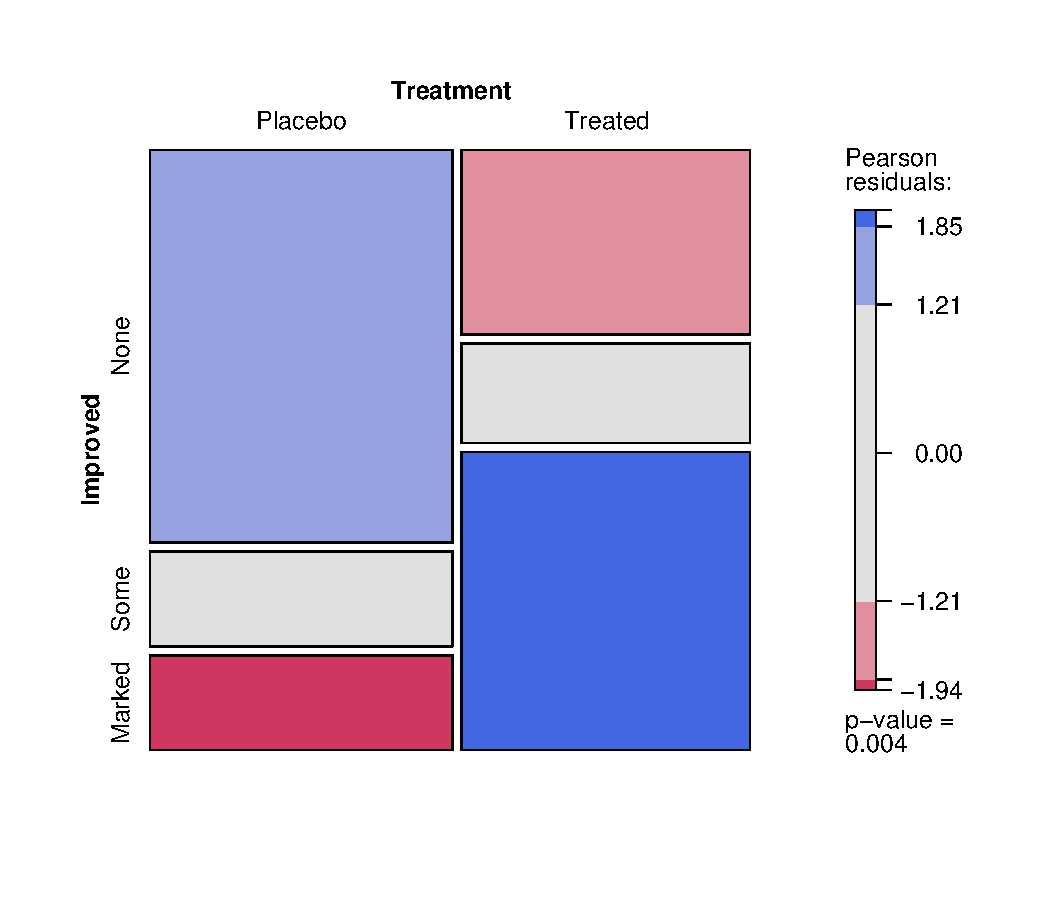
\includegraphics{strucplot-Arthritis}
\caption{Mosaic plot for the \data{Arthritis} data.}
\label{fig:arthritis}
\end{center}
\end{figure}

\setkeys{Gin}{width=\textwidth}
\begin{figure}[p]
\begin{center}
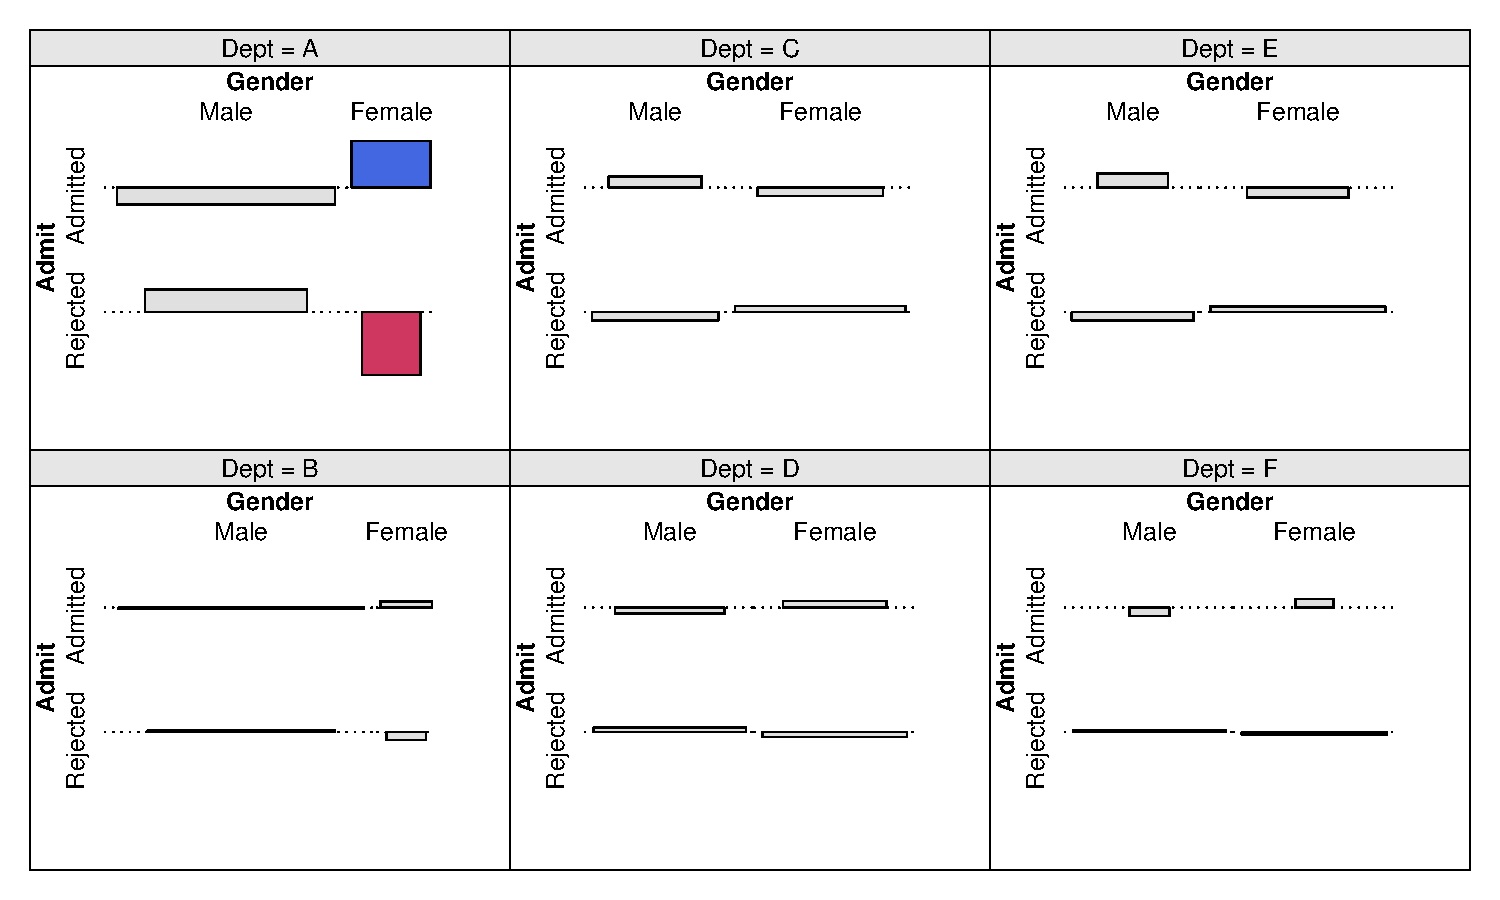
\includegraphics{strucplot-UCBAdmissions}
\caption{Conditional association plot for the \data{UCBAdmissions} data.}
\label{fig:ucbadmissions}
\end{center}
\end{figure}

\setkeys{Gin}{width=0.7\textwidth}
\begin{figure}[p]
\begin{center}
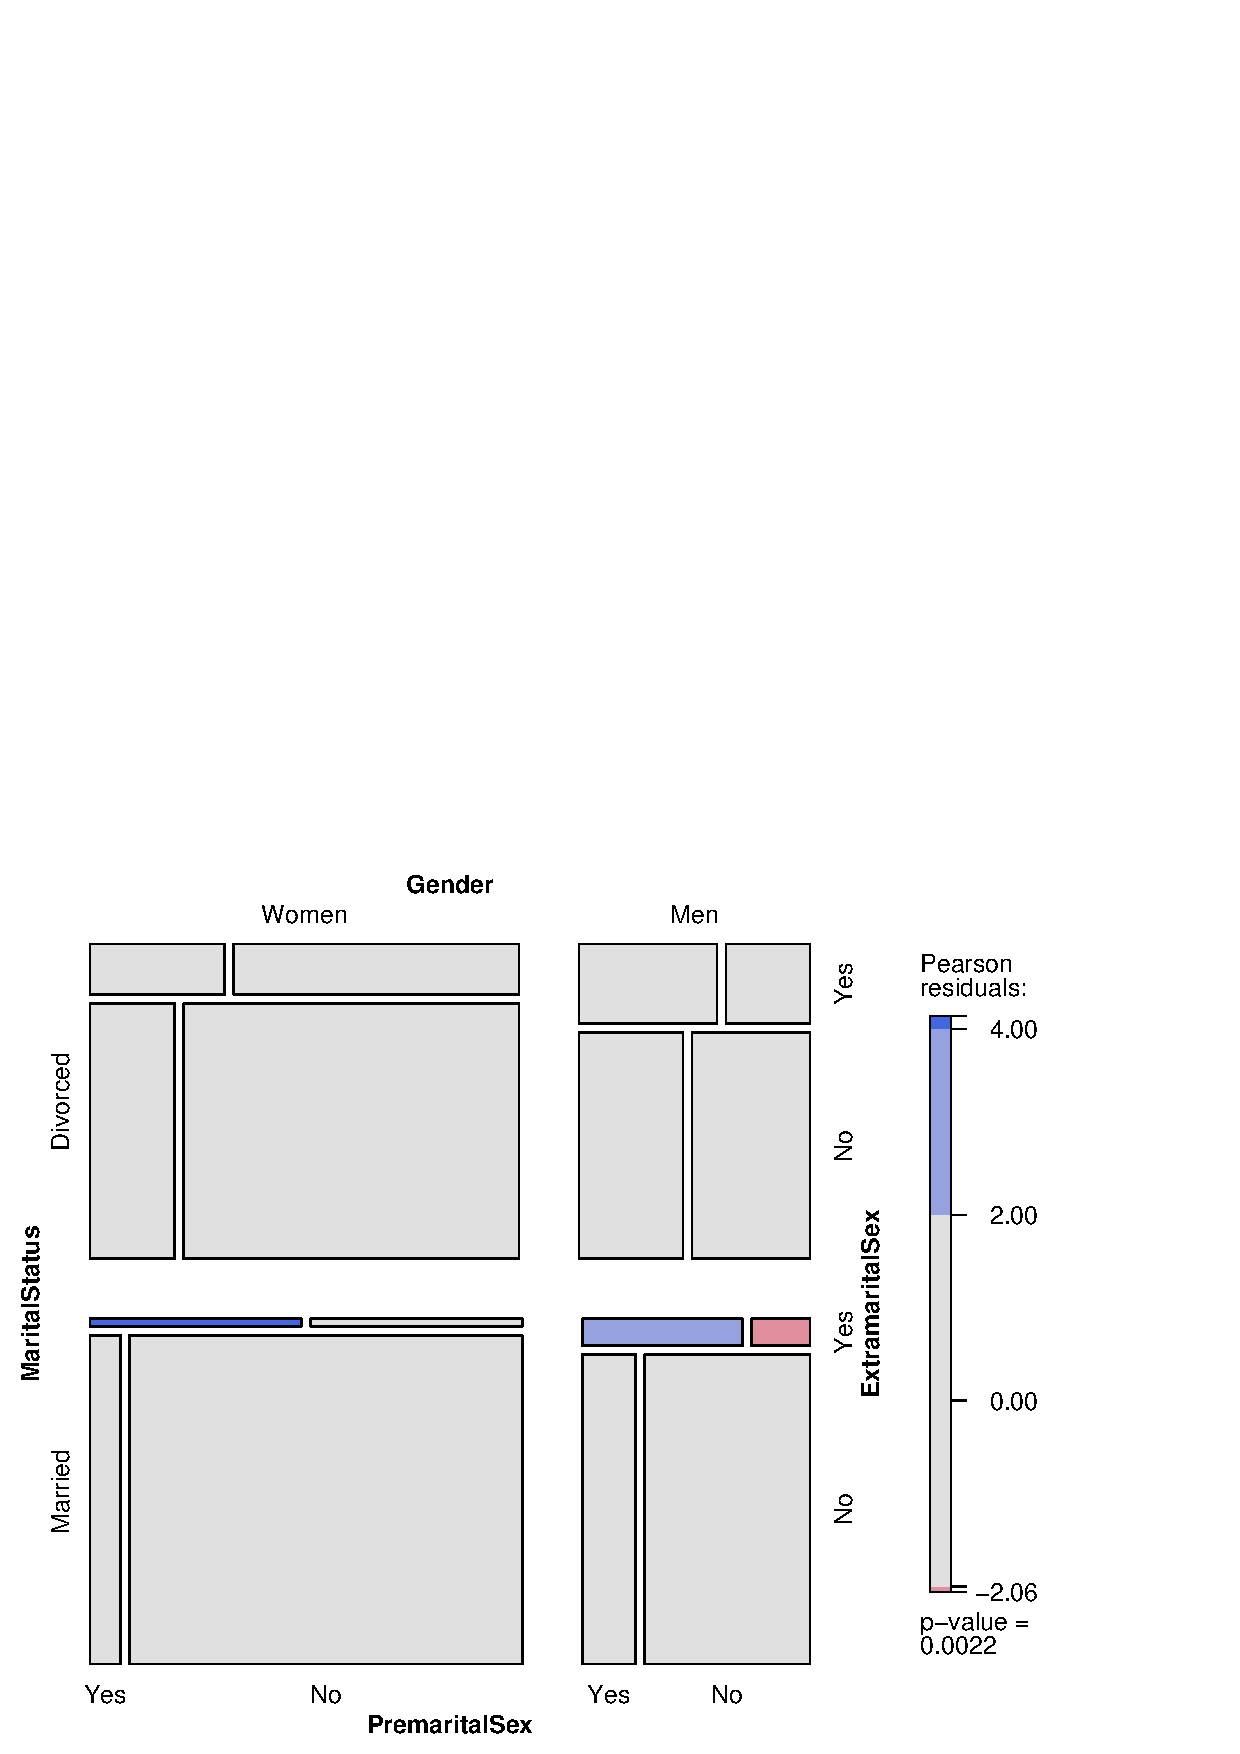
\includegraphics{strucplot-PreSex}
\caption{Mosaic plot for the \data{PreSex} data.}
\label{fig:presex}
\end{center}
\end{figure}

\setkeys{Gin}{width=0.8\textwidth}
\begin{figure}[p]
\begin{center}
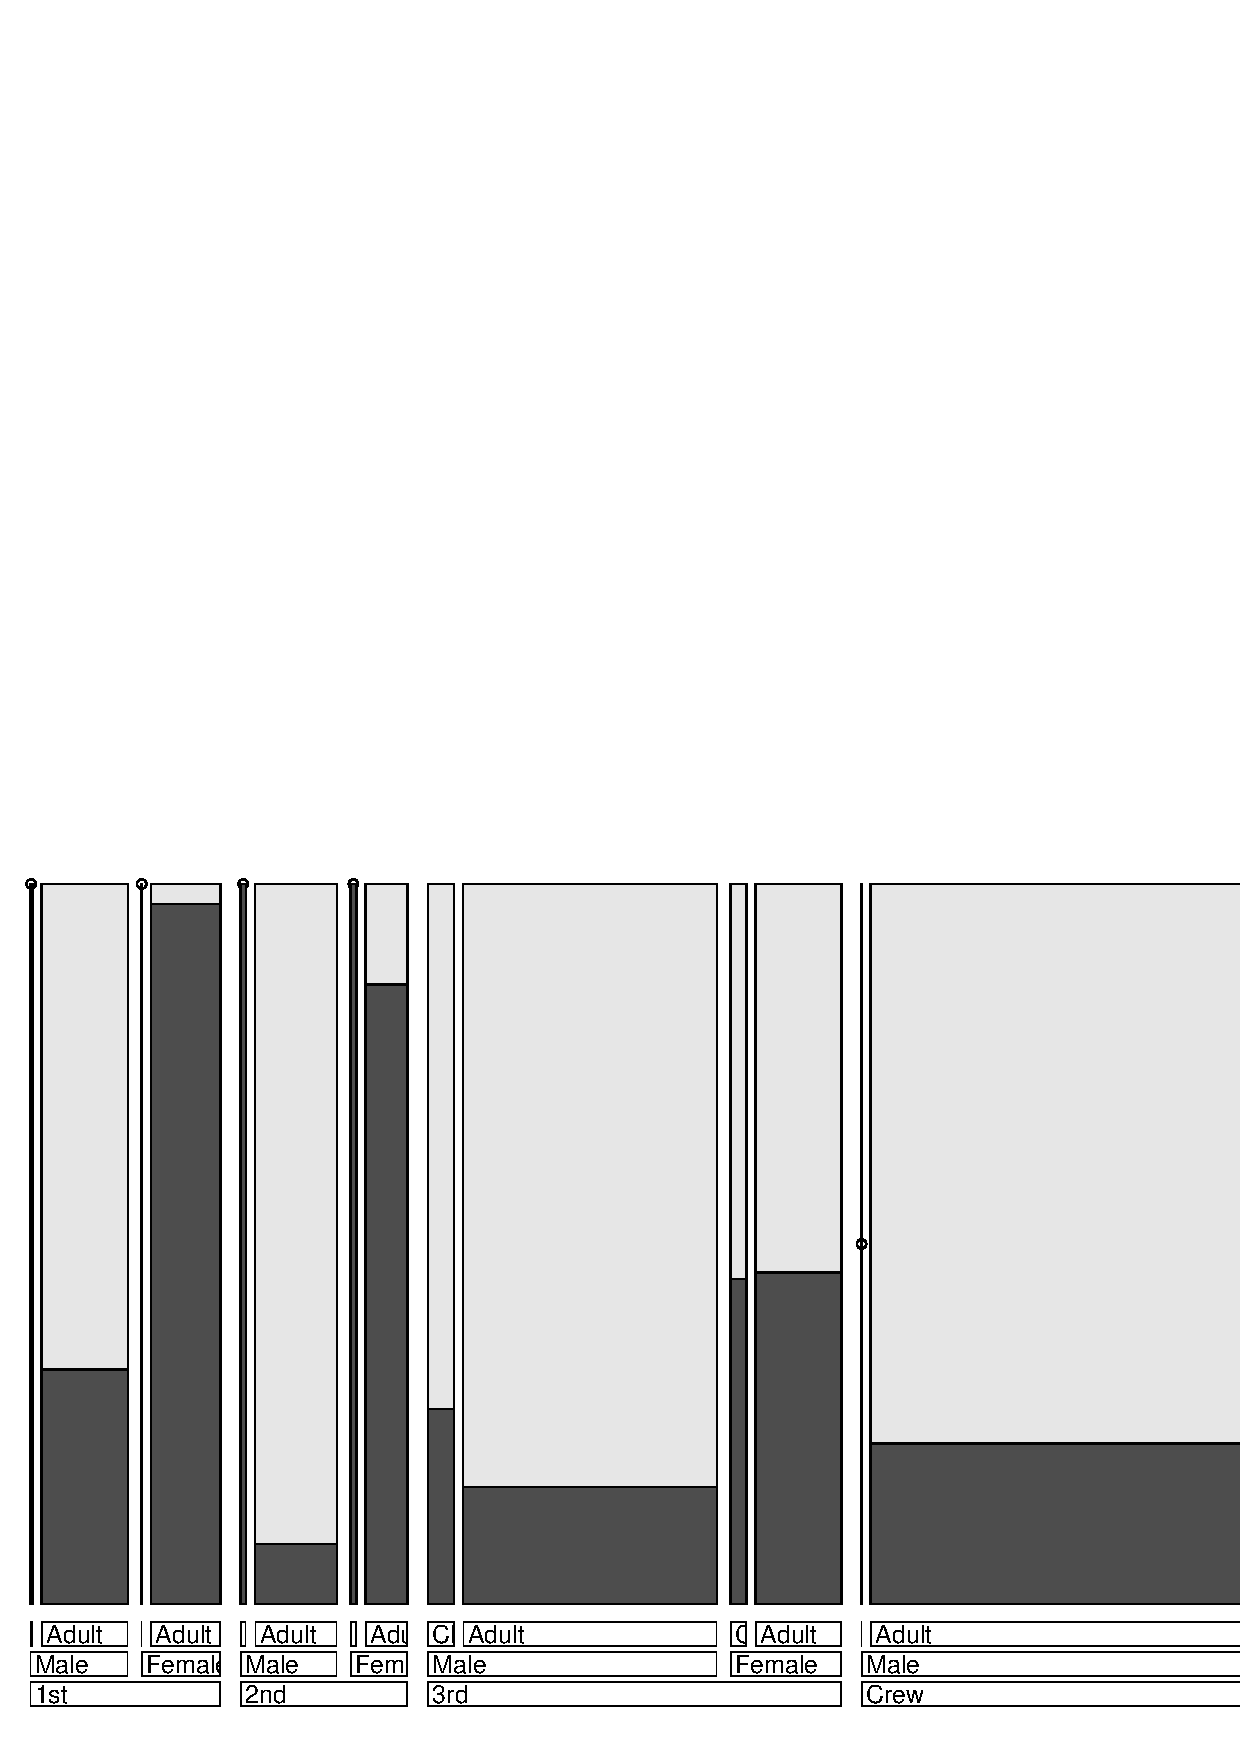
\includegraphics{strucplot-Titanic}
\caption{Double-decker plot for the \data{Titanic} data.}
\label{fig:titanic}
\end{center}
\end{figure}

This paper describes the strucplot framework provided by the \pkg{vcd}
package for the \proglang{R} environment for statistical computing and
graphics, available from the Comprehensive \proglang{R} Archive Network
(\url{http://CRAN.R-project.org/}).  The framework integrates displays
such as mosaic, association, and sieve plots by their unifying property
of being flat representations of contingency tables.  These basic plots,
as well as specialized displays for conditional independence, can be
used both for exploratory visualization and model-based analysis.
Exploratory techniques include specialized displays for the bivariate
case, as well as pairs and trellis-type displays for
higher-dimensional tables. Model-based tools include methods suitable
for the visualization of conditional independence tests (including
permutation tests), as well as for the visualization of particular GLMs
(logistic regression, log-linear models). Additionally, two of the
framework's further strengths are its flexibility and extensibility:
graphical appearance aspects such as shading, labeling, and spacing are
modularized by means of ``\underline{\vphantom{g}gr}aphical 
\underline{\vphantom{g}ap}pearance \underline{\vphantom{g}con}trol''
(\emph{grapcon}) functions, allowing
fine-granular customization and user-level extensions.

The remainder of the paper is organized as follows. In
Section \ref{sec:strucplot}, we give an overview of the strucplot
framework, describing the hierarchy of the main components and the
basic functionality. 
In Section \ref{sec:shading}, we demonstrate how
(residual-based) shadings support the visualization of log-linear models and
the results of independence tests. Also, we explain step-by-step how
the concepts of generating and grapcon functions
can be combined to provide a flexible customization of
complex graphical displays as created by the strucplot framework.
Sections \ref{sec:labeling} and \ref{sec:spacing} discuss in detail the labeling
and spacing features, respectively. Section \ref{sec:example}
exemplifies the framework in the analysis of a four-way data set.
Section \ref{sec:conclusion} concludes the work.

\section[The strucplot framework]{The strucplot framework}
\label{sec:strucplot}

The strucplot framework in the \proglang{R} package \pkg{vcd}, used for visualizing
multi-way contingency tables, integrates techniques such as
mosaic displays, association plots, and sieve plots. The main idea is to visualize
the tables' cells arranged in rectangular form. For multi-way tables,
the variables are nested into rows and columns using recursive
conditional splits, given the margins. The result is a 
``flat'' representation that can be visualized in
ways similar to a two-dimensional table.
This principle defines a class of conditional displays which allows
for granular control of graphical appearance aspects, including:

\begin{itemize}
\item the content of the tiles
\item the split direction for each dimension
\item the graphical parameters of the tiles' content
\item the spacing between the tiles
\item the labeling of the tiles
\end{itemize}

The strucplot framework is highly modularized: Figure~\ref{fig:struc}
shows the hierarchical relationship between the various components. 
On the lowest level, there are several groups of workhorse and 
parameter functions that directly or indirectly influence the final
appearance of the plot (see Table \ref{tab:grapcons} for an overview). 
These are examples of grapcon functions. They are created by generating functions
(\emph{grapcon generators}), allowing
flexible parameterization and extensibility (Figure~\ref{fig:struc}
only shows the generators). The generator names
follow the naming convention \code{\textit{group\_foo}()},  
where \code{\textit{group}} reflects the group the
generators belong to (strucplot core, labeling,
legend, shading, or spacing). The workhorse functions (created by 
\code{struc\_\textit{foo}()}, 
\code{labeling\_\textit{foo}()}, and \code{legend\_\textit{foo}()}) 
directly produce graphical output (i.e., ``add ink to the canvas''), whereas
the parameter functions
(created by \code{spacing\_\textit{foo}()} and \code{shading\_\textit{foo}()}) compute
graphical parameters used by the others. The grapcon functions returned by 
\code{struc\_\textit{foo}()} implement the core functionality, 
creating the tiles and their
content.  On the second level of the framework, a suitable combination
of the low-level grapcon functions (or, alternatively, corresponding generating functions)
is passed as ``hyperparameters'' to \codefun{strucplot}.
This central function 
sets up the graphical layout using grid viewports (see Figure~\ref{fig:layout}),
and coordinates the specified core, labeling, shading, and spacing functions to produce 
the plot. On the third level, we provide
several convenience functions such as \codefun{mosaic},
\codefun{sieve}, \codefun{assoc}, and \codefun{doubledecker} which 
interface \codefun{strucplot} through sensible parameter defaults
and support for model formulae. Finally, on the fourth
level, there are ``related'' \pkg{vcd} functions (such as \codefun{cotabplot}
and the \codefun{pairs} methods for table objects) 
arranging collections of plots of the strucplot 
framework into more complex displays (e.g., by means of panel functions).

\begin{table}
  \begin{tabular}{|l|l|l|}
    \hline
    \textbf{Group} & \textbf{Grapcon generator} & \textbf{Description}\\\hline
    strucplot & \codefun{struc\_assoc} & core function for association plots\\
    core      & \codefun{struc\_mosaic} & core function for mosaic plots\\
              & \codefun{struc\_sieve} & core function for sieve plots\\\hline\hline
     labeling & \codefun{labeling\_border} & border labels\\
              & \codefun{labeling\_cboxed} & centered labels with
              boxes, all labels clipped,\\
              && and on top and left border\\
              & \codefun{labeling\_cells} & cell labels\\
              & \codefun{labeling\_conditional} & border labels 
                                                  for conditioning variables\\
              && and cell labels for conditioned variables\\
              & \codefun{labeling\_doubledecker} & draws labels for
              doubledecker plot\\
              & \codefun{labeling\_lboxed} & left-aligned labels with boxes\\
              & \codefun{labeling\_left} & left-aligned border labels\\
              & \codefun{labeling\_left2} & left-aligned border
              labels, all labels on top and left border\\
              & \codefun{labeling\_list} & draws a list of labels
              under the plot\\\hline\hline
     shading  & \codefun{shading\_binary} & visualizes the sign of the  residuals\\
              & \codefun{shading\_Friendly} & implements Friendly
              shading (based on HSV colors)\\
              & \codefun{shading\_hcl} & shading based on HCL colors\\
              & \codefun{shading\_hsv} & shading based on HSV colors\\
              & \codefun{shading\_max} & shading visualizing the
              maximum test statistic\\ && (based on HCL colors)\\
              & \codefun{shading\_sieve} & implements Friendly
              shading customized for sieve plots\\ && (based on HCL colors)\\\hline\hline
     spacing  & \codefun{spacing\_conditional} & increasing spacing
              for conditioning variables,\\&& equal spacing for
              conditioned variables\\
              & \codefun{spacing\_dimequal} & equal spacing for each dimension\\
              & \codefun{spacing\_equal} & equal spacing for all dimensions\\
              & \codefun{spacing\_highlighting} & increasing spacing,
              last dimension set to zero\\
              & \codefun{spacing\_increase} & increasing spacing\\\hline\hline
     legend   & \codefun{legend\_fixed} & creates a fixed number of
              bins (similar to \codefun{mosaicplot})\\
              & \codefun{legend\_resbased} & suitable for an
              arbitrary number of bins\\&& (also for continuous shadings)\\\hline

  \end{tabular}
  \caption{Available grapcon generators in the strucplot framework}
  \label{tab:grapcons}
\end{table}

\begin{figure}[h]
  \begin{center}
    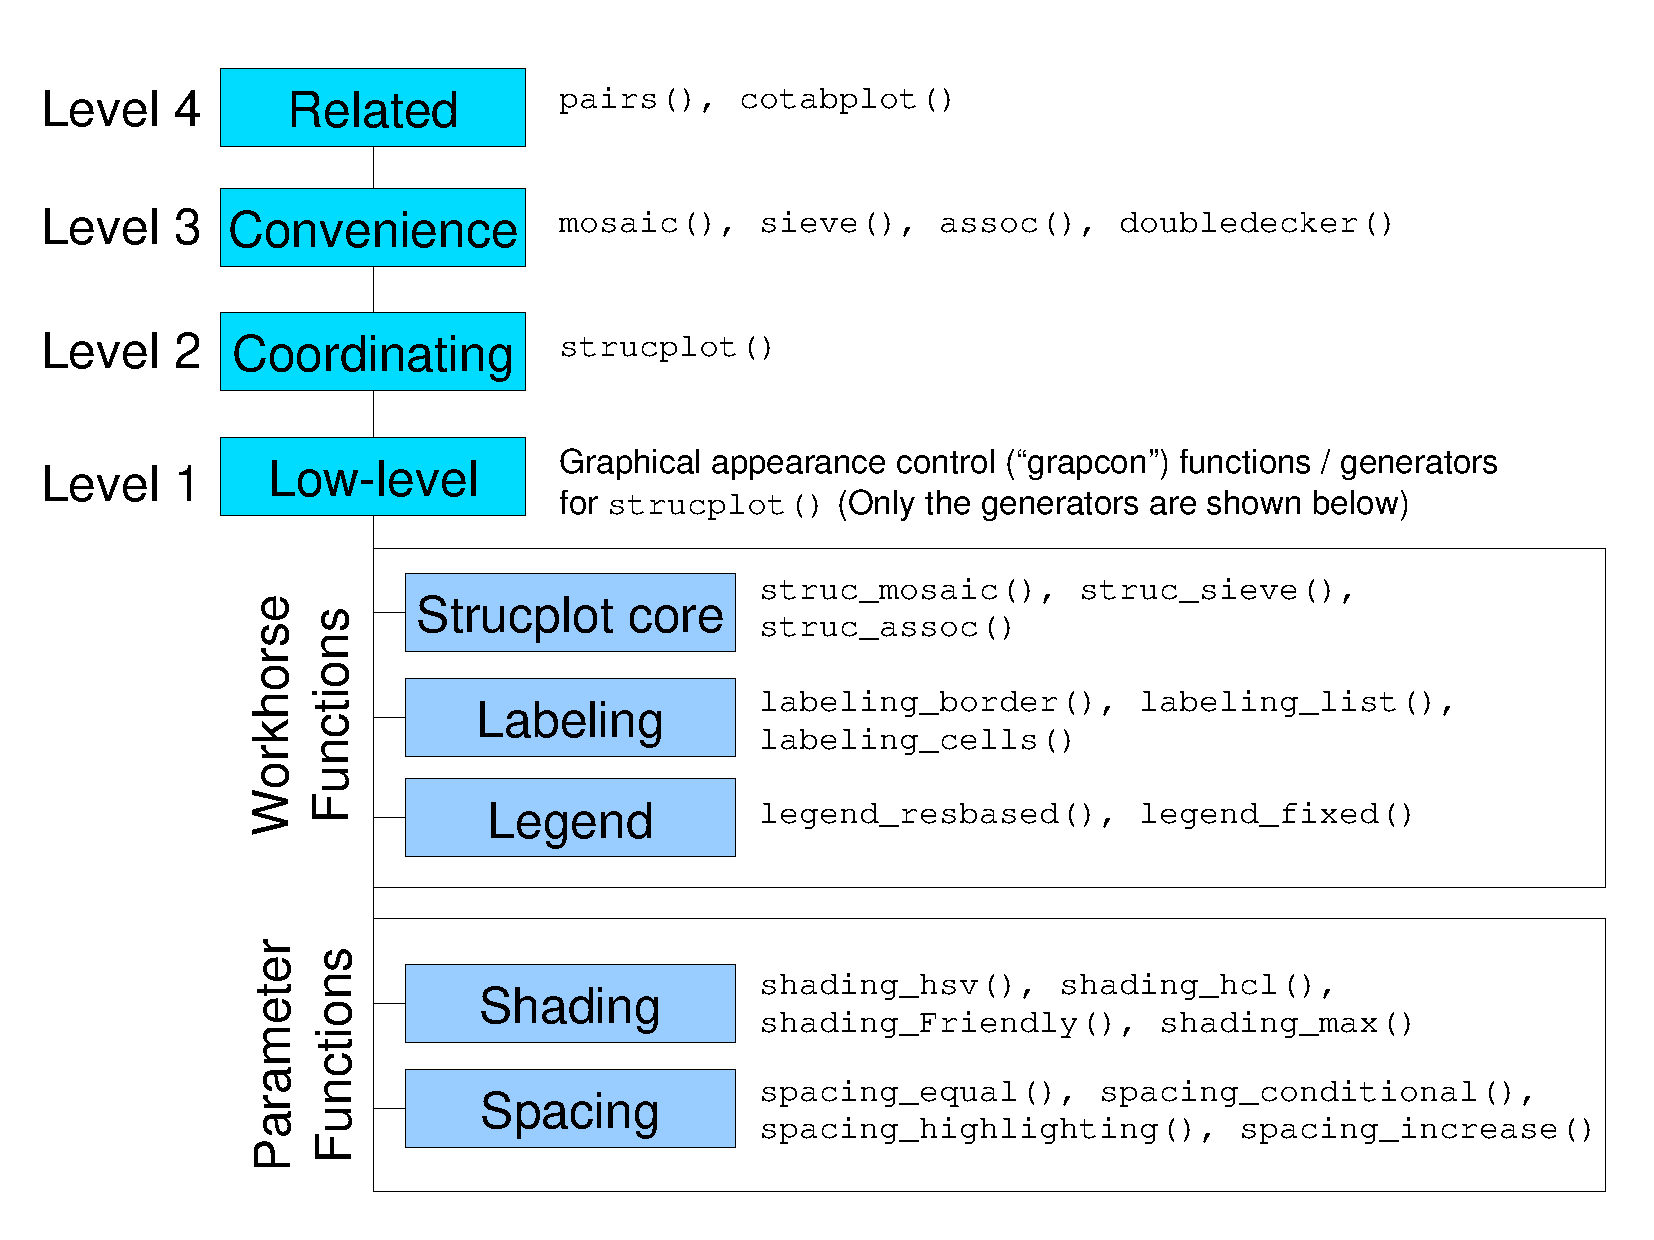
\includegraphics[width=0.8\textwidth]{struc}
    \caption{Components of the strucplot framework.}
    \label{fig:struc}
  \end{center}
\end{figure}

\setkeys{Gin}{width=0.6\textwidth}
\begin{figure}[h]
\begin{center}
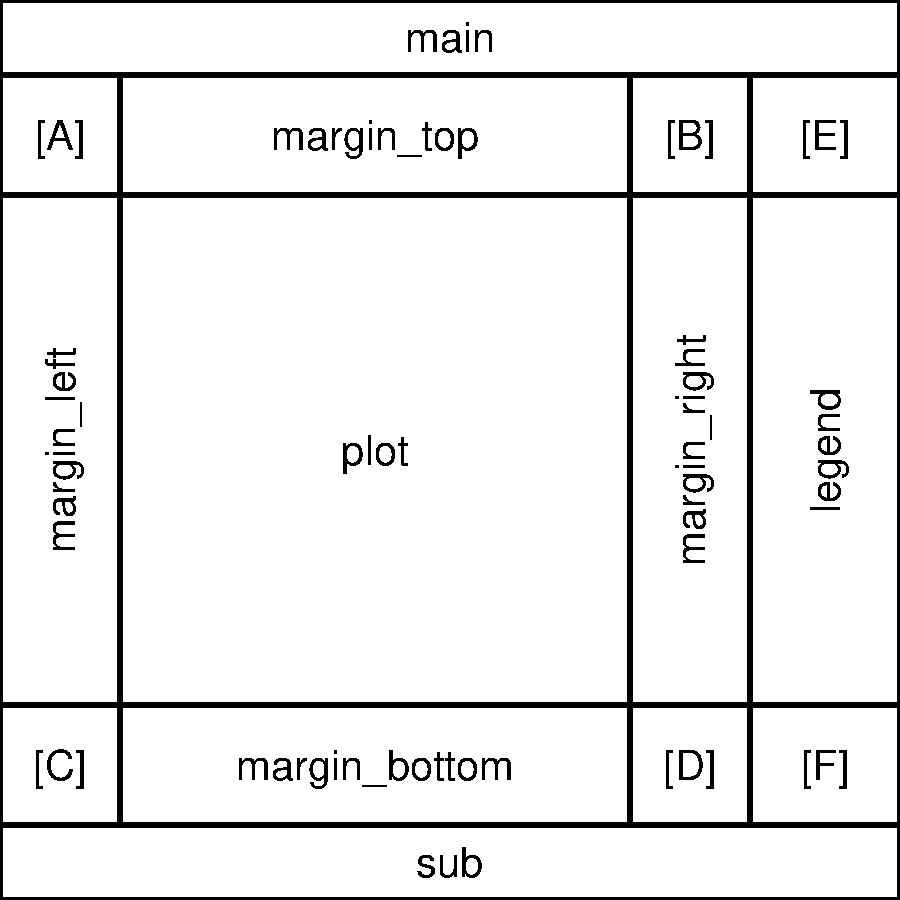
\includegraphics{strucplot-vcdlayout}
\caption{Viewport layout for strucplot displays with their names. [A] =
  ``corner\_top\_left'', [B] = ``corner\_top\_right'', 
  [C] = ``corner\_bottom\_left'', [D] = ``corner\_bottom\_right'', [E]
  = ``legend\_top'', [F] = ``legend\_sub''.}
\label{fig:layout}
\end{center}
\end{figure}
\setkeys{Gin}{width=0.7\textwidth}

\subsection{Mosaic, association, and sieve plots}

As an example, consider the \data{HairEyeColor} 
data containing two polytomous variables (hair and eye color), 
as well as one (artificial) dichotomous gender variable (\code{Sex}). The
``flattened'' contingency table can be obtained using the
\codefun{structable} function (quite similar to \codefun{ftable} in
base \proglang{R}, but allowing the specification of split directions):

\begin{Schunk}
\begin{Sinput}
> (HEC <- structable(Eye ~ Sex + Hair, data = HairEyeColor))
\end{Sinput}
\begin{Soutput}
             Eye Brown Blue Hazel Green
Sex    Hair                            
Male   Black        32   11    10     3
       Brown        38   50    25    15
       Red          10   10     7     7
       Blond         3   30     5     8
Female Black        36    9     5     2
       Brown        81   34    29    14
       Red          16    7     7     7
       Blond         4   64     5     8
\end{Soutput}
\end{Schunk}

Let us first visualize the contingency table by means of a mosaic plot.
% \citep{vcd:Hartigan+Kleiner:1984} which is basically 
% an area-proportional visualization of (typically, observed) frequencies, composed
% of tiles (corresponding to the cells) created by recursive
% vertical and horizontal splits of a square. Thus, the area of each tile
% is proportional to the corresponding cell entry \emph{given} the
% dimensions of previous splits. 
The effect of

\begin{Schunk}
\begin{Sinput}
> mosaic(HEC)
\end{Sinput}
\end{Schunk}

\noindent equivalent to

\begin{Schunk}
\begin{Sinput}
> mosaic(~Sex + Eye + Hair, data = HairEyeColor)
\end{Sinput}
\end{Schunk}

%\setkeys{Gin}{width=0.75\textwidth}
\begin{figure}[p]
\begin{center}
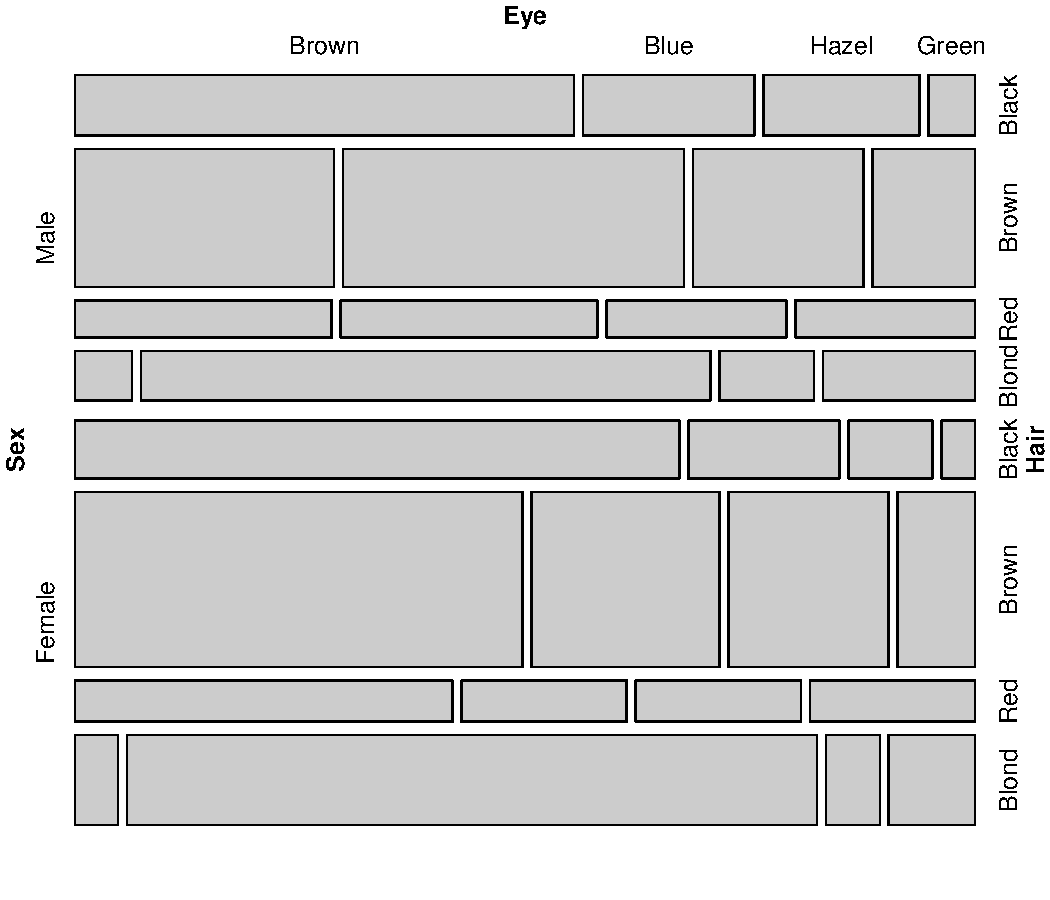
\includegraphics{strucplot-Observedfig}
\caption{Mosaic plot for the \data{HairEyeColor} data.}
\label{fig:observed}
\end{center}
\end{figure}

\noindent depicts the observed frequencies of the \code{HairEyeColor}
data. If there are zero entries, tiles have zero area and are, additionally,
marked by small bullets (see, e.g, Figure~\ref{fig:titanic}). By
default, these cells are not split further. The bullets help
distinguishing very small cells from zero entries, and are
particularly useful when color shadings come into play 
(see the example using the \data{Bundesliga} data in Section \ref{sec:overview}). 
Note that in contrast to, e.g.,  \codefun{mosaicplot} in base
\proglang{R}, the default split direction and level ordering in all strucplot
displays correspond to the textual representation produced by the
print methods.
It is also possible to visualize the expected values instead of the
observed values (see Figure~\ref{fig:expected}):

\begin{Schunk}
\begin{Sinput}
> mosaic(HEC, type = "expected")
\end{Sinput}
\end{Schunk}

\begin{figure}[p]
\begin{center}
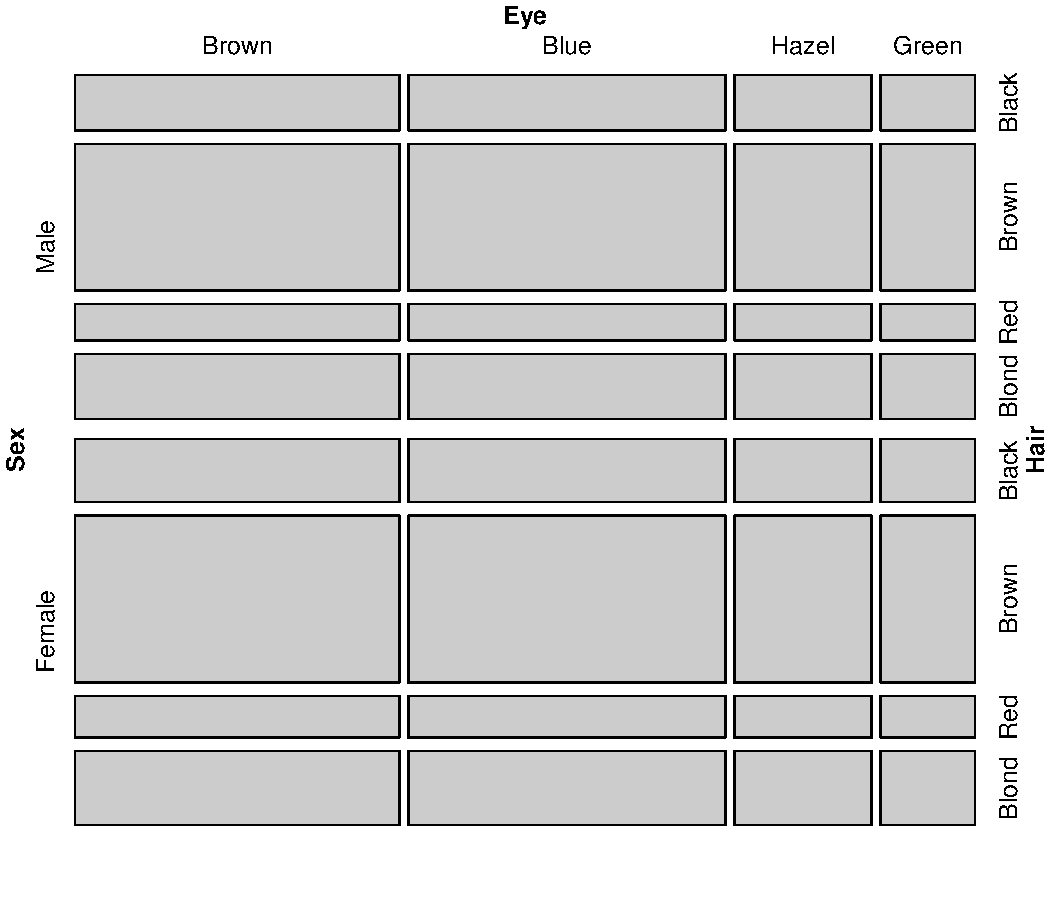
\includegraphics{strucplot-Expectedfig}
\caption{Mosaic plot for the \data{HairEyeColor} data (expected values).}
\label{fig:expected}
\end{center}
\end{figure}
%\setkeys{Gin}{width=0.7\textwidth}

\noindent In order to compare observed and expected values,
a sieve plot \citep{vcd:riedwyl+schuepbach:1994} 
could be used (see Figure~\ref{fig:sieve}):

\begin{Schunk}
\begin{Sinput}
> sieve(~Sex + Eye + Hair, data = HEC, spacing = spacing_dimequal(c(2, 
+     0, 0)))
\end{Sinput}
\end{Schunk}

\begin{figure}[h]
\begin{center}
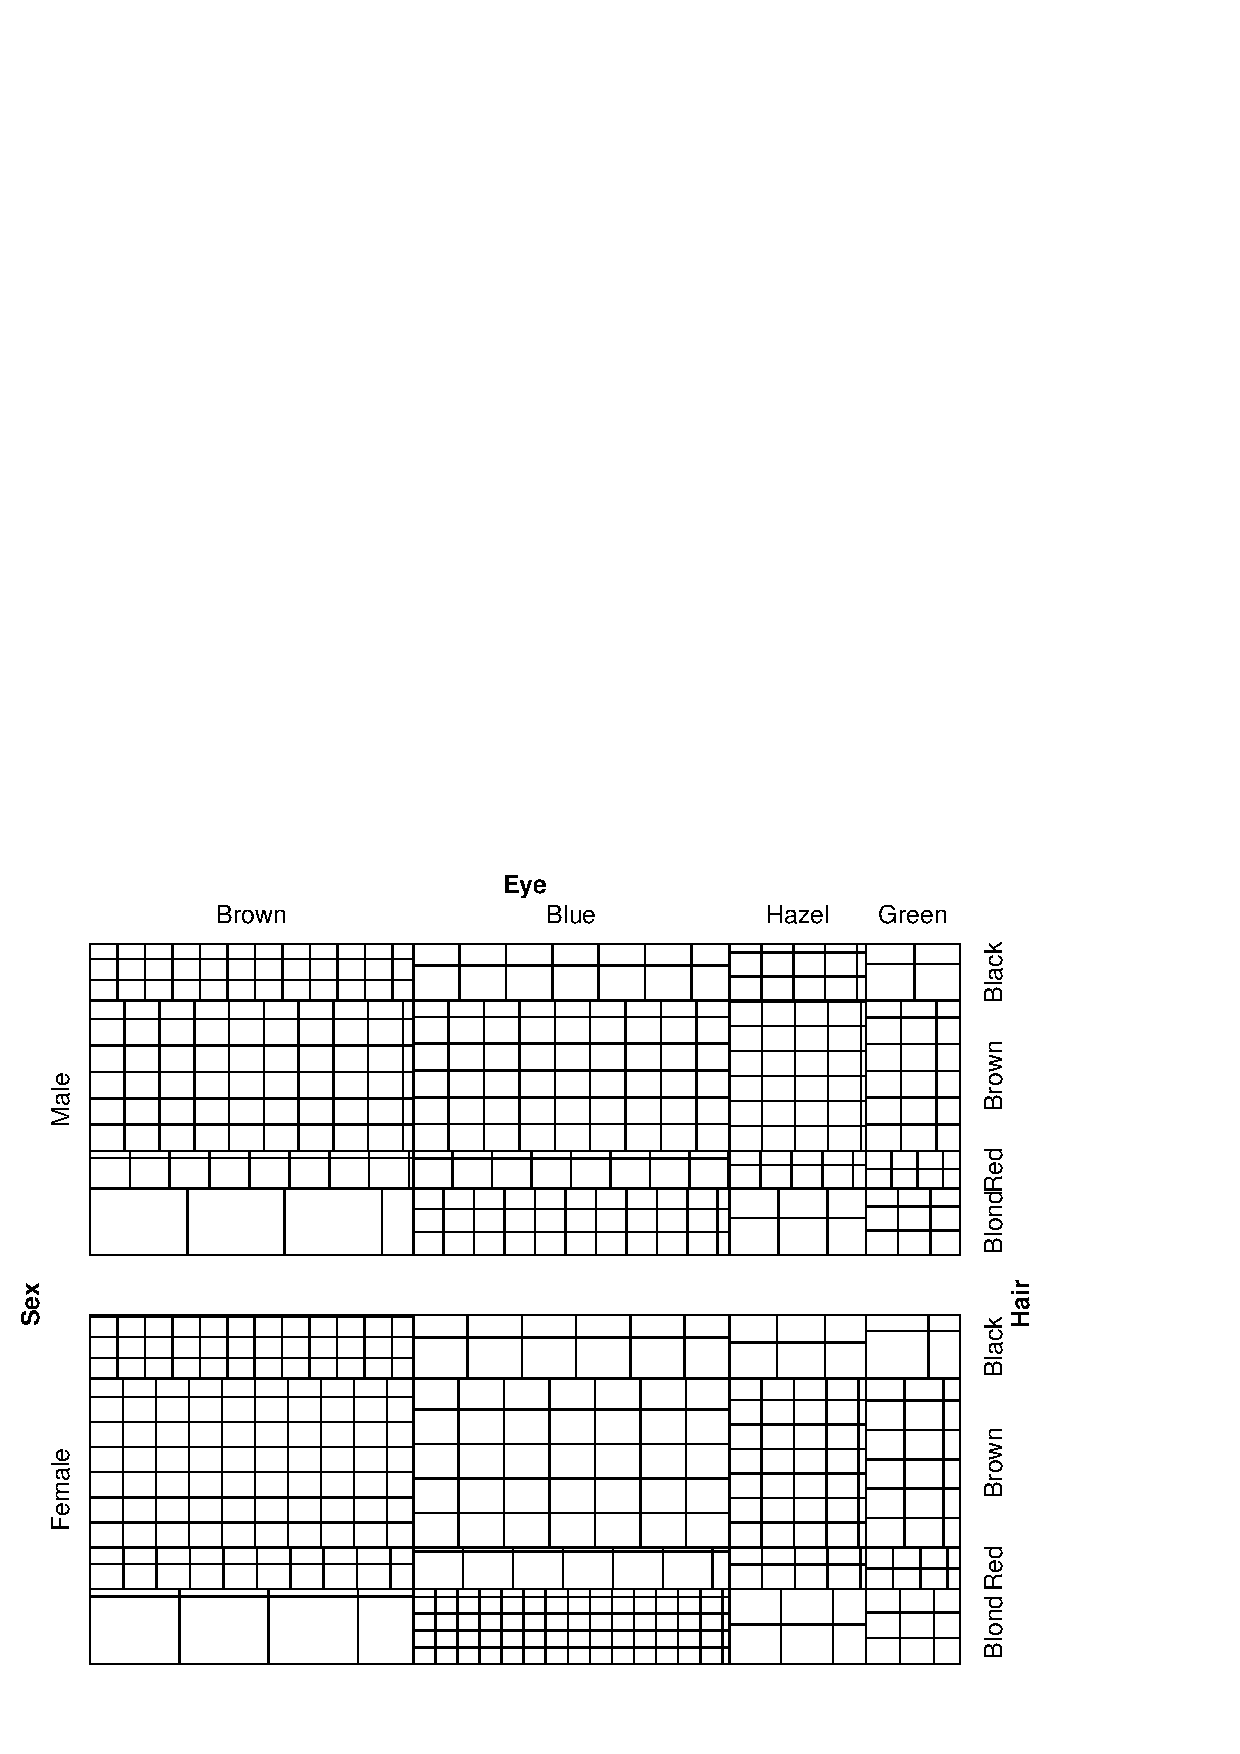
\includegraphics{strucplot-sievefig}
\caption{Sieve plot for the \data{HairEyeColor} data visualizing simultaneously
  observed and expected values.}
\label{fig:sieve}
\end{center}
\end{figure}

\noindent where \code{spacing\_dimequal} is used to set the spacing
of the second and third dimension to zero. Alternatively, we can directly inspect the residuals. 
The Pearson residuals (standardized deviations of observed from expected values) 
are conveniently visualized using association
plots \citep{vcd:Cohen:1980}. In contrast to \codefun{assocplot} in
base \proglang{R}, \pkg{vcd}'s \codefun{assoc}
function scales to more than two variables (see Figure~\ref{fig:residuals}):

\begin{Schunk}
\begin{Sinput}
> assoc(HEC, compress = FALSE)
\end{Sinput}
\end{Schunk}

\begin{figure}[p]
\begin{center}
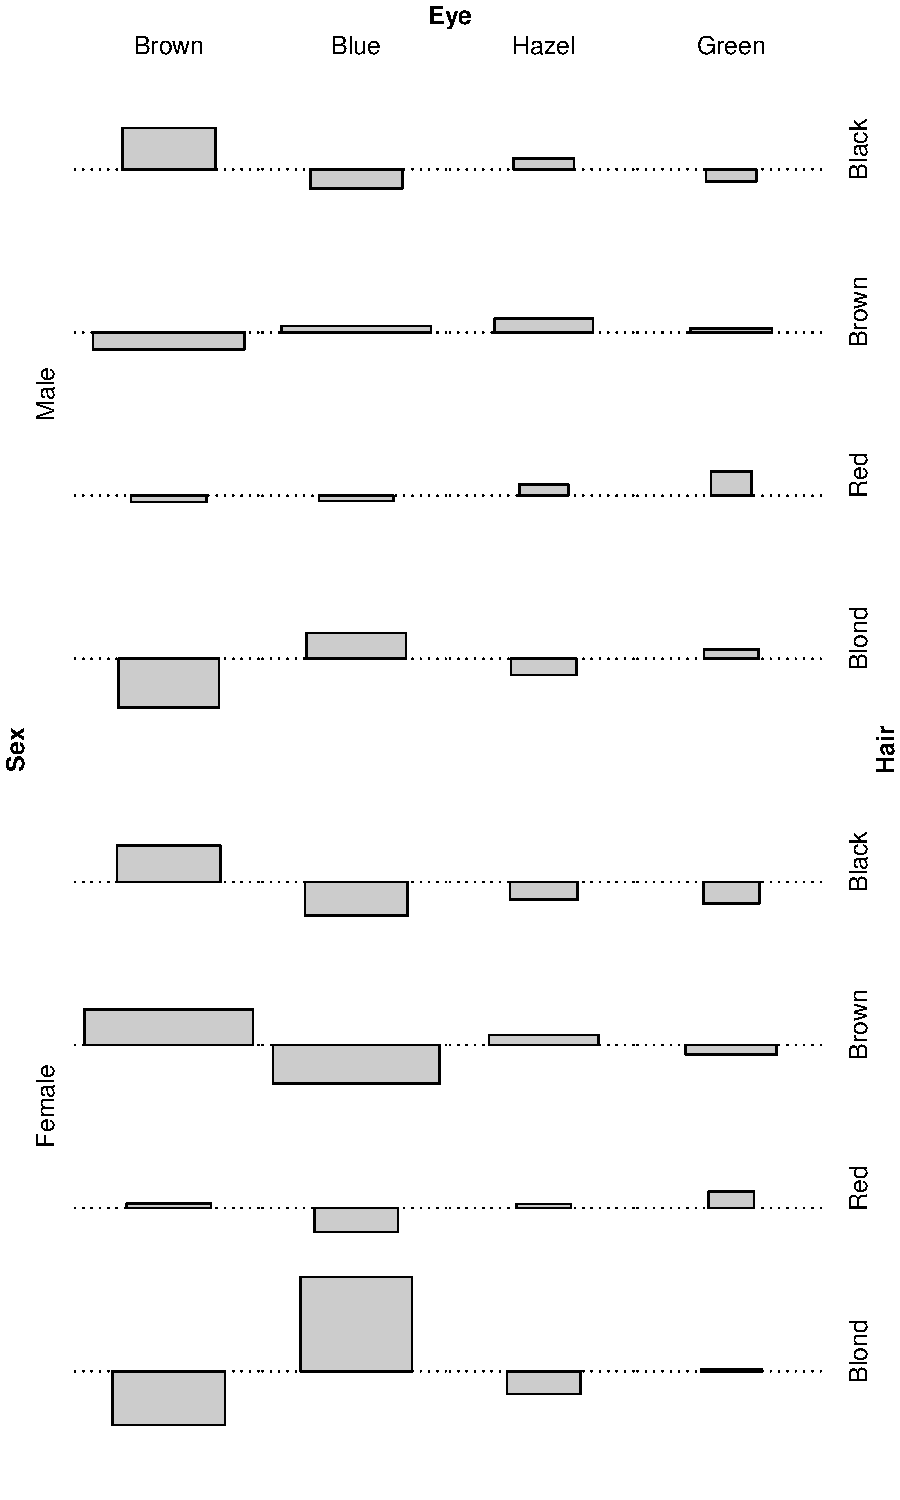
\includegraphics{strucplot-Residualsfig}
\caption{Association plot for the \data{HairEyeColor} data.}
\label{fig:residuals}
\end{center}
\end{figure}

\noindent where the \code{compress} argument keeps distances between tiles
equal.

For both mosaic plots and association plots, 
the splitting of the tiles can be controlled using the
\code{split\_vertical} argument. The default is to alternate splits starting
with a horizontal one (see Figure~\ref{fig:split}):


\begin{Schunk}
\begin{Sinput}
> mosaic(HEC, split_vertical = c(TRUE, FALSE, TRUE), 
+     labeling_args = list(abbreviate = c(Eye = 3)))
\end{Sinput}
\end{Schunk}


\begin{figure}[p]
\begin{center}
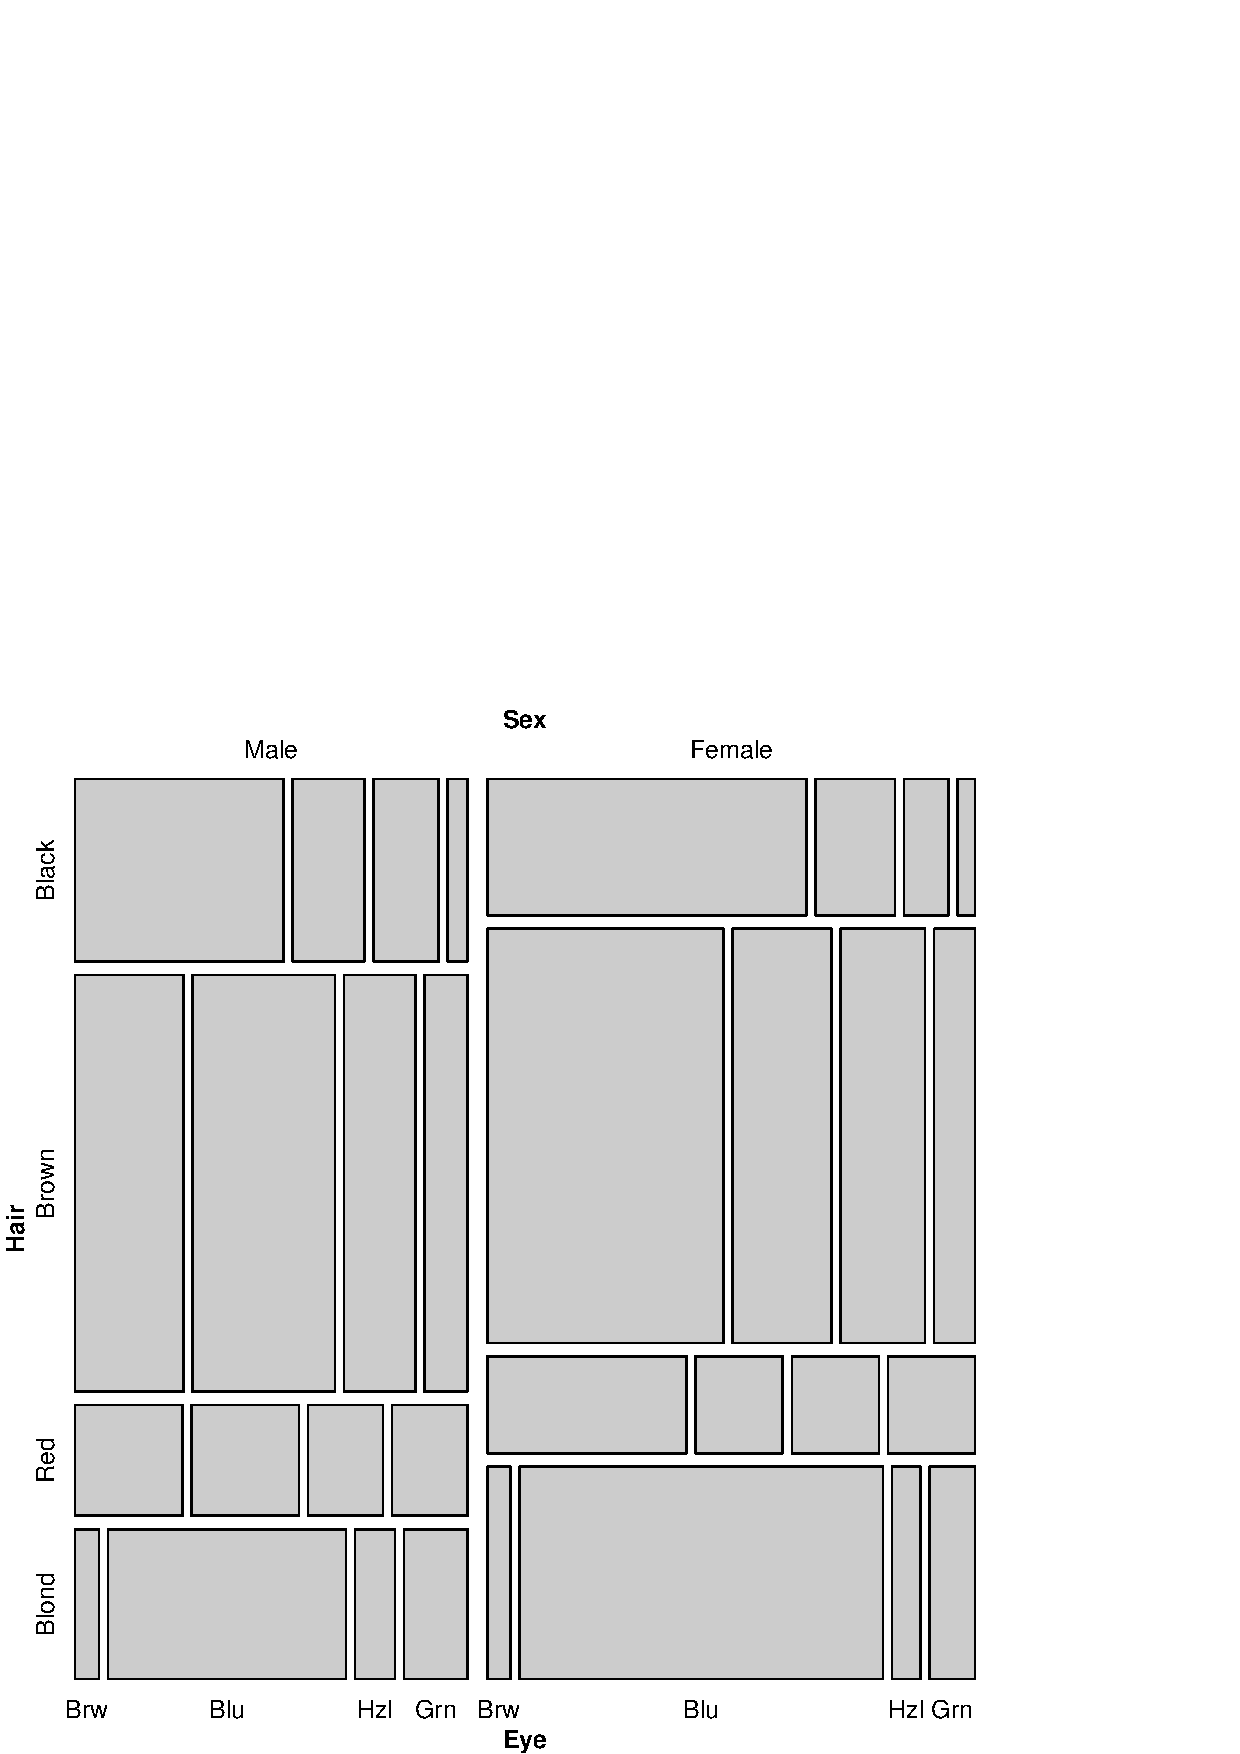
\includegraphics{strucplot-splitfig}
\caption{Mosaic plot for the \data{HairEyeColor} data---alternative splitting.}
\label{fig:split}
\end{center}
\end{figure}

\noindent (Note that \code{HEC}, a \class{structable} object, already
includes a splitting information which simply gets overloaded in this
example.)  For compatibility with \codefun{mosaicplot} in base
\proglang{R}, the \codefun{mosaic} function also allows the use of a
\code{direction} argument taking a vector of \code{"h"} and \code{"v"}
characters:

\begin{Schunk}
\begin{Sinput}
> mosaic(HEC, direction = c("v", "h", "v"))
\end{Sinput}
\end{Schunk}

By a suitable combination of splitting, spacing, and
labeling settings, the functions provided by the strucplot framework
can be customized in a quite flexible way. For example, 
the default method for \codefun{doubledecker} is simply a wrapper for 
\codefun{strucplot}, setting the right defaults.
Most default settings such as colors, spacing, and labeling are
specified via the parameters and passed through to
\codefun{strucplot}. The additional code just handles the dependent
variable information, and in particular permutes the table to have the dependent
variable as the last dimension as required for the doubledecker plot.
Figure~\ref{fig:titanic} shows a doubledecker plot of
the \data{Titanic} data, explaining the probability of survival (``survived'') by age, given
sex, given class. It is created by:

\begin{Schunk}
\begin{Sinput}
> doubledecker(Titanic)
\end{Sinput}
\end{Schunk}

\noindent equivalent to:

\begin{Schunk}
\begin{Sinput}
> doubledecker(Survived ~ Class + Sex + Age, data = Titanic)
\end{Sinput}
\end{Schunk}

\subsection{Conditional and partial views}


So far, we have visualized either full or collapsed tables, as
suggested by the analysis task at hand. Subtables can be selected in a
similar way as for objects of class \class{table} using
indexing. Note, however, that subsetting of \class{structable} objects 
is more restrictive because of their inherent conditional structure. Since the variables
on both the row and the columns side are nested, 
subsetting is only possible ``outside-in'', that is, indexing operates
on blocks defined by the variable levels. In the following, we use the
Titanic data again, this time collapsed over \code{Survived} to investigate the
structure of crew and passengers (and having the \code{Child} and
\code{Age} labels of the \code{Age} variable swapped for optical clarity):


\begin{Schunk}
\begin{Sinput}
> (STD <- structable(~Sex + Class + Age, data = Titanic[, , 
+     2:1, ]))
\end{Sinput}
\begin{Soutput}
             Class 1st 2nd 3rd Crew
Sex    Age                         
Male   Adult       175 168 462  862
       Child         5  11  48    0
Female Adult       144  93 165   23
       Child         1  13  31    0
\end{Soutput}
\begin{Sinput}
> STD["Male", ]
\end{Sinput}
\begin{Soutput}
           Class 1st 2nd 3rd Crew
Sex  Age                         
Male Adult       175 168 462  862
     Child         5  11  48    0
\end{Soutput}
\begin{Sinput}
> STD["Male", c("1st", "2nd", "3rd")]
\end{Sinput}
\begin{Soutput}
           Class 1st 2nd 3rd
Sex  Age                    
Male Adult       175 168 462
     Child         5  11  48
\end{Soutput}
\end{Schunk}


\noindent \emph{Conditioning} on levels (i.e., choosing a table subset for fixed levels
of the conditioning variable(s)) is done using the \code{[[} operator. %]]
Here again, the sequence of conditioning levels is restricted by the
hierarchical structure of the \class{structable} object. In the
following examples, note that compared to subsetting, the first
dimension(s) are dropped:

\begin{Schunk}
\begin{Sinput}
> STD[["Male", ]]
\end{Sinput}
\begin{Soutput}
      Class 1st 2nd 3rd Crew
Age                         
Adult       175 168 462  862
Child         5  11  48    0
\end{Soutput}
\begin{Sinput}
> STD[[c("Male", "Adult"), ]]
\end{Sinput}
\begin{Soutput}
Class 1st 2nd 3rd Crew
                      
      175 168 462  862
\end{Soutput}
\begin{Sinput}
> STD[["Male", "1st"]]
\end{Sinput}
\begin{Soutput}
Age       
Adult  175
Child    5
\end{Soutput}
\end{Schunk}

\noindent Now, there are several ways for visualizing 
conditional independence structures. The ``brute force'' method is to
draw separate plots for the strata. The following example compares 
the association between hair and eye color, given gender, by using
subsetting on the flat table and \pkg{grid}'s viewport 
framework to visualize the two groups besides each other:

\begin{Schunk}
\begin{Sinput}
> pushViewport(viewport(layout = grid.layout(ncol = 2)))
\end{Sinput}
\end{Schunk}

\begin{Schunk}
\begin{Sinput}
> pushViewport(viewport(layout.pos.col = 1))
> mosaic(STD[["Male"]], margins = c(left = 2.5, top = 2.5, 
+     0), sub = "Male", newpage = FALSE)
> popViewport()
\end{Sinput}
\end{Schunk}

\begin{Schunk}
\begin{Sinput}
> pushViewport(viewport(layout.pos.col = 2))
> mosaic(STD[["Female"]], margins = c(top = 2.5, 0), sub = "Female", 
+     newpage = FALSE)
> popViewport(2)
\end{Sinput}
\end{Schunk}

\setkeys{Gin}{width=\textwidth}
\begin{figure}[p]
\begin{center}
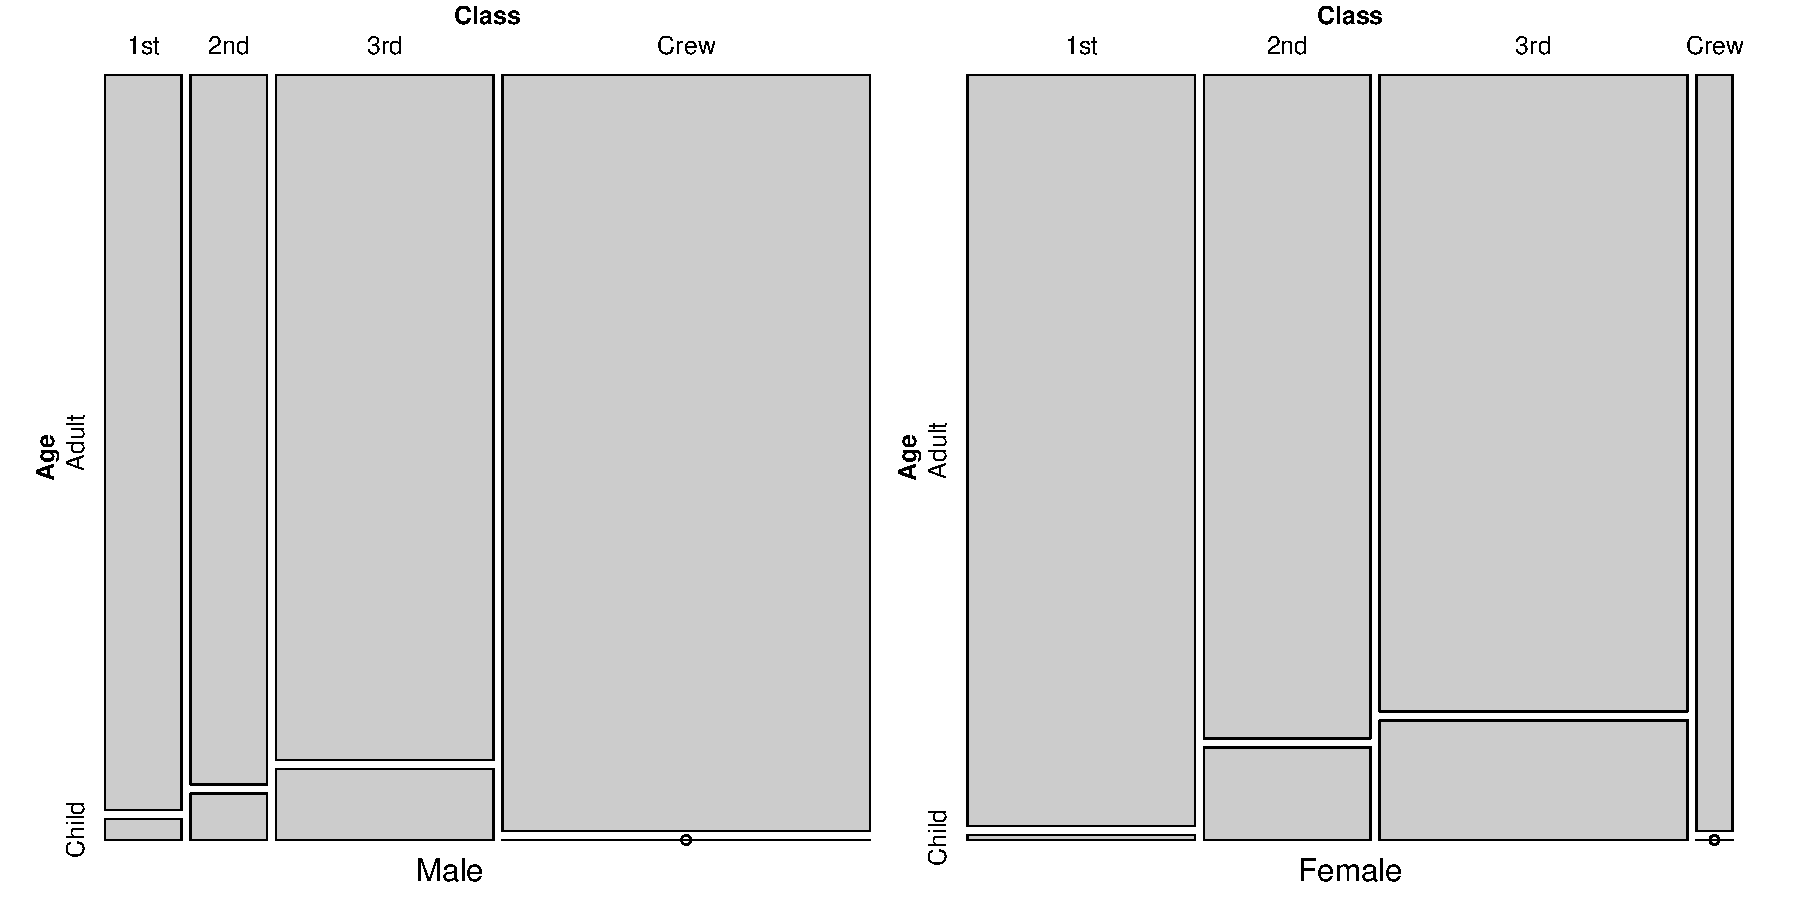
\includegraphics{strucplot-Variablesfig}
\caption{Two mosaic displays put side-by-side, visualizing the 
distribution of class and age, given gender. The marginal
distribution of gender cannot be seen.}
\label{fig:parttable}
\end{center}
\end{figure}
\setkeys{Gin}{width=0.7\textwidth}

\noindent Note the use of the \code{margins} argument: it takes a
vector with up to four values whose unnamed components are recycled,
but ``overruled'' by the named arguments. Thus, in the second example, only
the top margin is set to 2.5 lines, and all other to 0.
This idea applies to almost all
vectorized arguments in the strucplot framework (with
\code{split\_vertical} as a prominent exception).

The \codefun{cotabplot} function does a much better job on this task:
it arranges stratified strucplot displays 
in a lattice-like layout, conditioning on variable \emph{levels}.
The plot in Figure~\ref{fig:cotabplot} shows hair and eye color, given sex:

\begin{Schunk}
\begin{Sinput}
> cotabplot(~Class + Age | Sex, data = STD, split_vertical = TRUE)
\end{Sinput}
\end{Schunk}

\setkeys{Gin}{width=\textwidth}
\begin{figure}[p]
\begin{center}
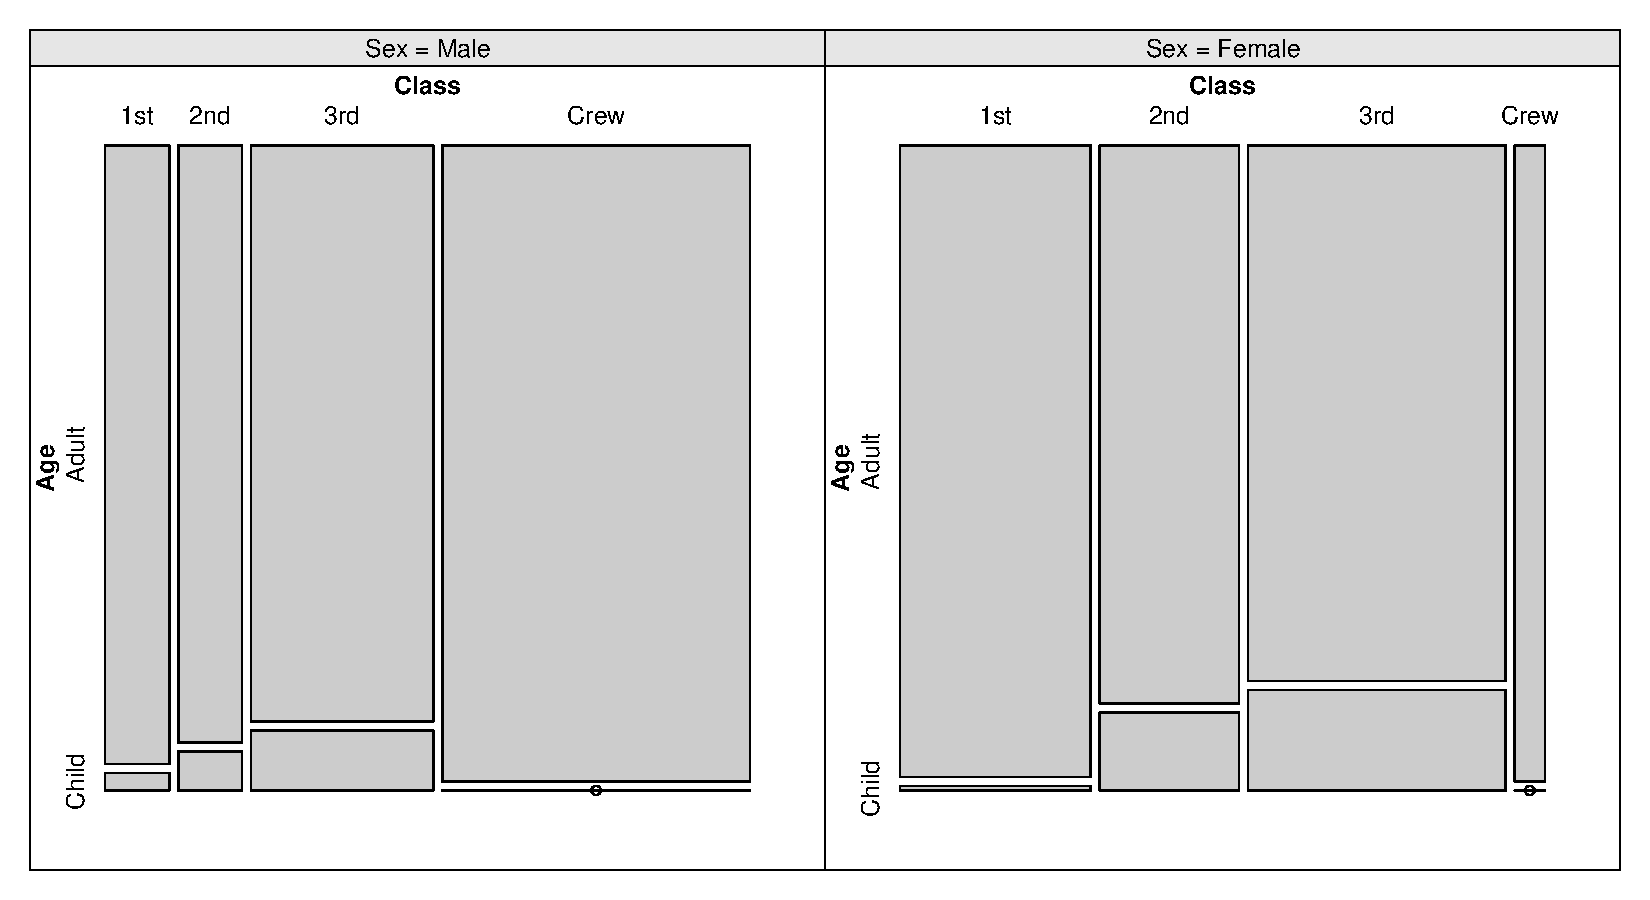
\includegraphics{strucplot-cotabplotfig}
\caption{Conditional table plot for the \data{Titanic} data,
  again visualizing the distribution of age and class, given
  gender, using separate mosaic displays like the ``manual'' plot 
  in Figure~\ref{fig:parttable}.}
\label{fig:cotabplot}
\end{center}
\end{figure}
\setkeys{Gin}{width=0.7\textwidth}
%\noindent The \code{labeling\_args} argument modifies the labels'
%appearance: here, to be left-aligned and unclipped
%(see Section \ref{sec:labeling}).

\noindent Visualizing the strata separately ``hides'' the distribution of the
conditioning variable(s) which may or may not be appropriate or
sensible in a particular analysis step. If we wish to keep the
information on the marginal distribution(s), we can use one single
mosaic for the stratified plot since mosaic displays are 
``conditional plots'' by definition. We just need to make sure that
conditioning variables are used first for splitting. 
Both the default and the formula interface of \codefun{mosaic} allow the
specification of conditioning variables (see Figure~\ref{fig:conditioning}):

\begin{Schunk}
\begin{Sinput}
> mosaic(STD, condvars = "Sex", split_vertical = c(TRUE, 
+     TRUE, FALSE))
\end{Sinput}
\end{Schunk}
\begin{Schunk}
\begin{Sinput}
> mosaic(~Class + Age | Sex, data = STD, split_vertical = c(TRUE, 
+     TRUE, FALSE))
\end{Sinput}
\end{Schunk}

\setkeys{Gin}{width=\textwidth}
\begin{figure}[h]
\begin{center}
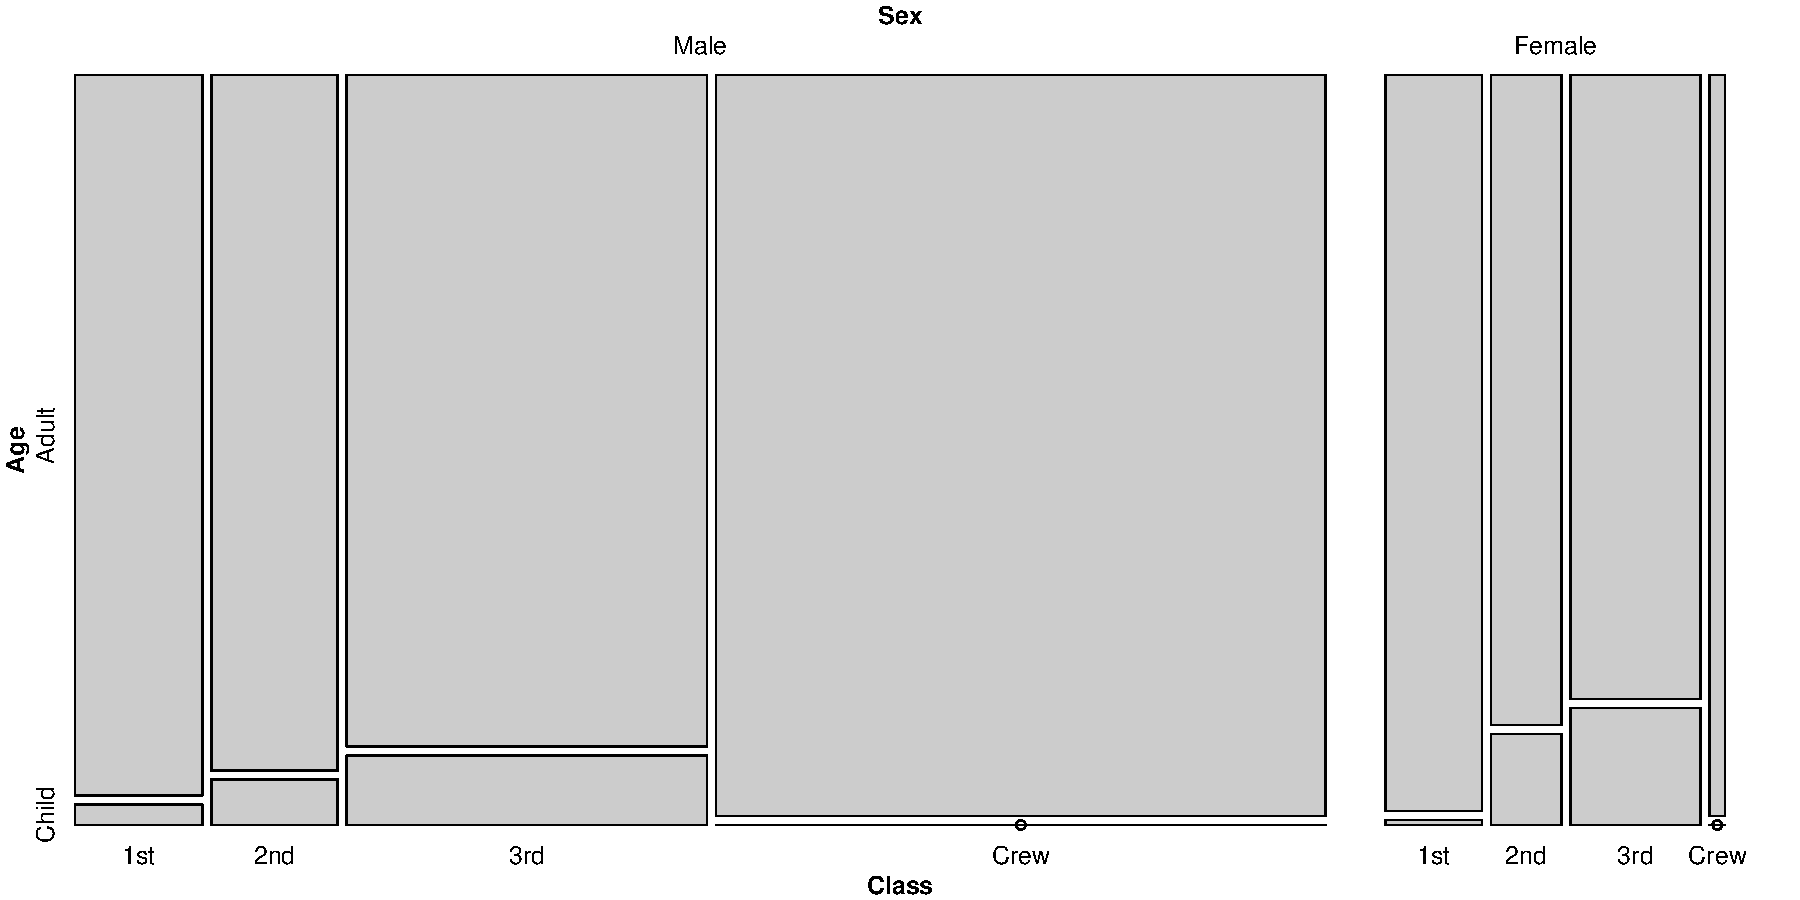
\includegraphics{strucplot-Conditioningfig}
\caption{Mosaic plot again visualizing the 
distribution of class and age, given gender, this time using a
single mosaic plot. In contrast to Figures~\ref{fig:parttable} and \ref{fig:cotabplot}, 
this plot also visualizes the marginal distribution of gender.}
\label{fig:conditioning}
\end{center}
\end{figure}
\setkeys{Gin}{width=0.7}

\noindent The effect of using this is that
conditioning variables are permuted ahead of the the conditioned variables
in the table, and that \codefun{spacing\_conditional} is used as default to better
distinguish conditioning from conditioned dimensions.
This spacing uses equal space between tiles of conditioned variables,
and increasing space between tiles of conditioning variables (See 
Section~\ref{sec:spacing}).

Another set of high-level functions for visualizing conditional independence
models are the \codefun{pairs} methods for \class{table} and \class{structable} objects.
In contrast to \codefun{cotabplot} which conditions on variables,
the \codefun{pairs} methods create pairwise views of the table. 
They produce, by default, a plot matrix 
having strucplot displays in the off-diagonal panels, and
the variable names (optionally, with univariate displays) in the diagonal cells. 
Figure~\ref{fig:pairs} shows a pairs display for the
\data{Titanic} data with univariate mosaics in the diagonal,
and mosaic plots visualizing the corresponding bivariate mosaics
in the upper and lower triangles.
Due to the inherent asymmetry of mosaic displays, the corresponding plots in the
upper and lower triangle differ depending on which variable is used first
for splitting---inspecting both views might help detecting patterns in a data set. 
Additionally, 
we are using a special spacing and shading normally used to `highlight' %'
the second variable in the first (as will be discussed in Section \ref{sec:spacing}): here,
the intention of the spacing 
is to emphasize the conditional distributions of the second variable,
given the first one, and the shading helps identifying the factor levels in
the second variable.

\begin{Schunk}
\begin{Sinput}
> pairs(STD, highlighting = 2, diag_panel = pairs_diagonal_mosaic, 
+     diag_panel_args = list(fill = grey.colors))
\end{Sinput}
\end{Schunk}


%\setkeys{Gin}{width=\textwidth}
\setkeys{Gin}{width=0.7\textwidth}
\begin{figure}[h]
\begin{center}
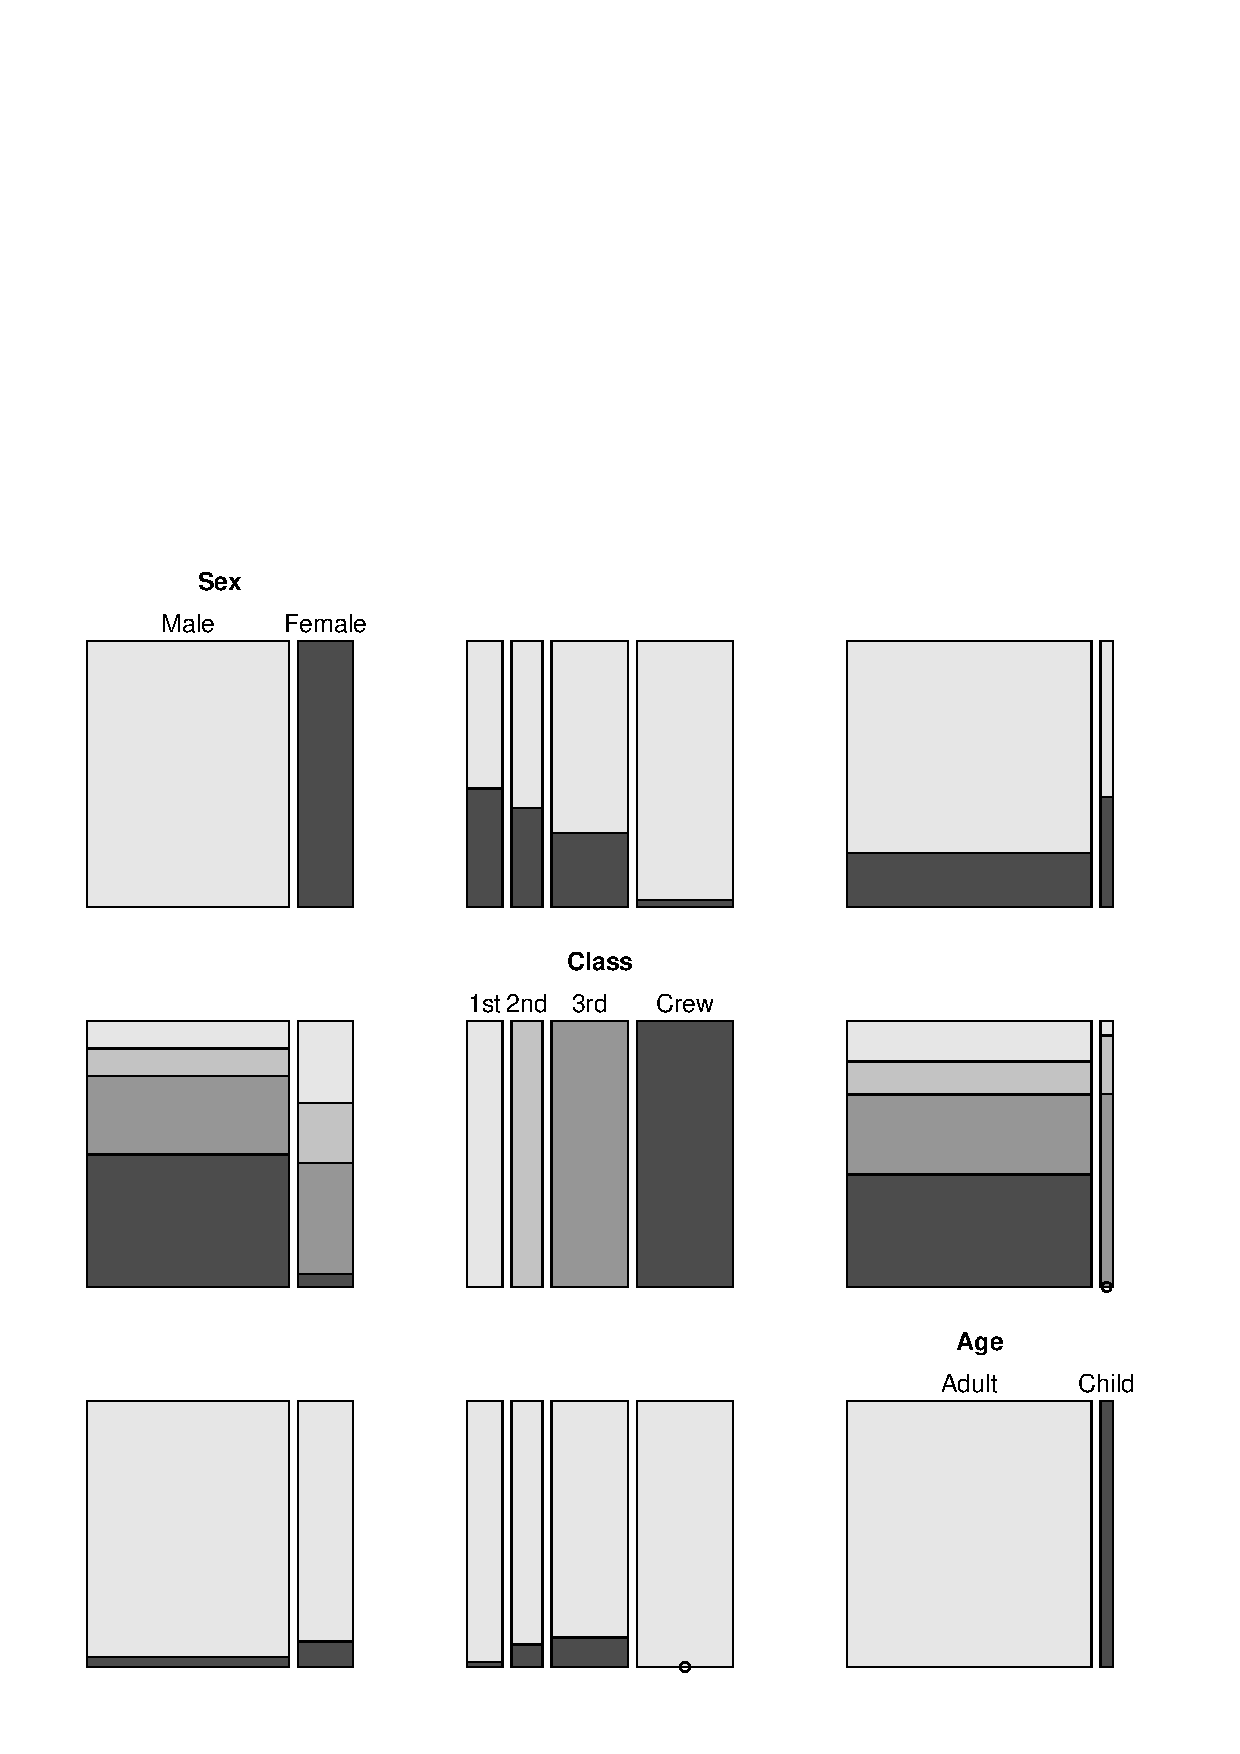
\includegraphics{strucplot-pairsfig}
\caption{Pairs plot for the \data{Titanic} data.}
\label{fig:pairs}
\end{center}
\end{figure}
\setkeys{Gin}{width=0.7\textwidth}

\noindent The labels of the variables are to be read from left to
right and from top to bottom. In addition, the levels can be matched
by position within the columns and by shading within the rows.
In plots produced by \codefun{pairs}, 
each panel's row and column define two variables $X$ and $Y$ used for the
specification of four different types of independence: pairwise,
total, conditional, and joint. The pairwise mosaic
matrix shows bivariate marginal relations between $X$ and $Y$, collapsed over all
other variables. The total independence mosaic matrix shows mosaic
plots for mutual independence, i.e., for marginal and conditional independence
among all pairs of variables. The conditional
independence mosaic matrix shows mosaic plots for marginal
independence of $X$ and $Y$, given all other variables. The joint independence
mosaic matrix shows mosaic plots for joint independence of all
pairs ($X$, $Y$) of variables from the others.

Upper and lower parts can
independently be used to display different 
types of independence models, or different strucplot displays
(mosaic, association, or sieve plots).
The available panel functions (\codefun{pairs\_assoc}, 
\codefun{pairs\_mosaic}, and \codefun{pairs\_sieve}) 
are simple wrappers to \codefun{assoc}, 
\codefun{mosaic}, and \codefun{sieve}, respectively. 
Obviously, seeing patterns in strucplot matrices 
becomes increasingly difficult with
higher dimensionality. Therefore, this plot is typically used with a suitable 
residual-based shading (see Section \ref{sec:shading}).

\subsection{Interactive plot modifications}

All strucplot core functions are supposed to produce conditional
hierarchical plots by the means of nested viewports, corresponding to
the provided splitting information. Thus, at the end of the plotting,
each tile is associated with a particular viewport. Each of those
viewports has to be conventionally named, enabling other strucplot
modules, in particular the labeling functions, to access specific tiles
after they have been plotted. The naming convention for the viewports
is:

\begin{center}
\code{\emph{[Optional prefix]}cell:\emph{Variable1}=\emph{Level1},\emph{Variable2}=\emph{Level2}} \dots
\end{center}

\noindent Clearly, these names depend on the splitting.
The following example shows how to access parts of the plot after it has
been drawn (see Figure~\ref{fig:afterplot}):

\begin{Schunk}
\begin{Sinput}
> mosaic(~Hair + Eye, data = HEC, pop = FALSE)
> seekViewport("cell:Hair=Blond")
> grid.rect(gp = gpar(col = "red", lwd = 4))
> seekViewport("cell:Hair=Blond,Eye=Blue")
> grid.circle(r = 0.2, gp = gpar(fill = "cyan"))
\end{Sinput}
\end{Schunk}

\noindent Note that the viewport tree is removed by
default. Therefore, the \texttt{pop} argument has to be set to
\texttt{FALSE} when viewports shall be accessed. 

\setkeys{Gin}{width=0.6\textwidth}
\begin{figure}[h]
\begin{center}
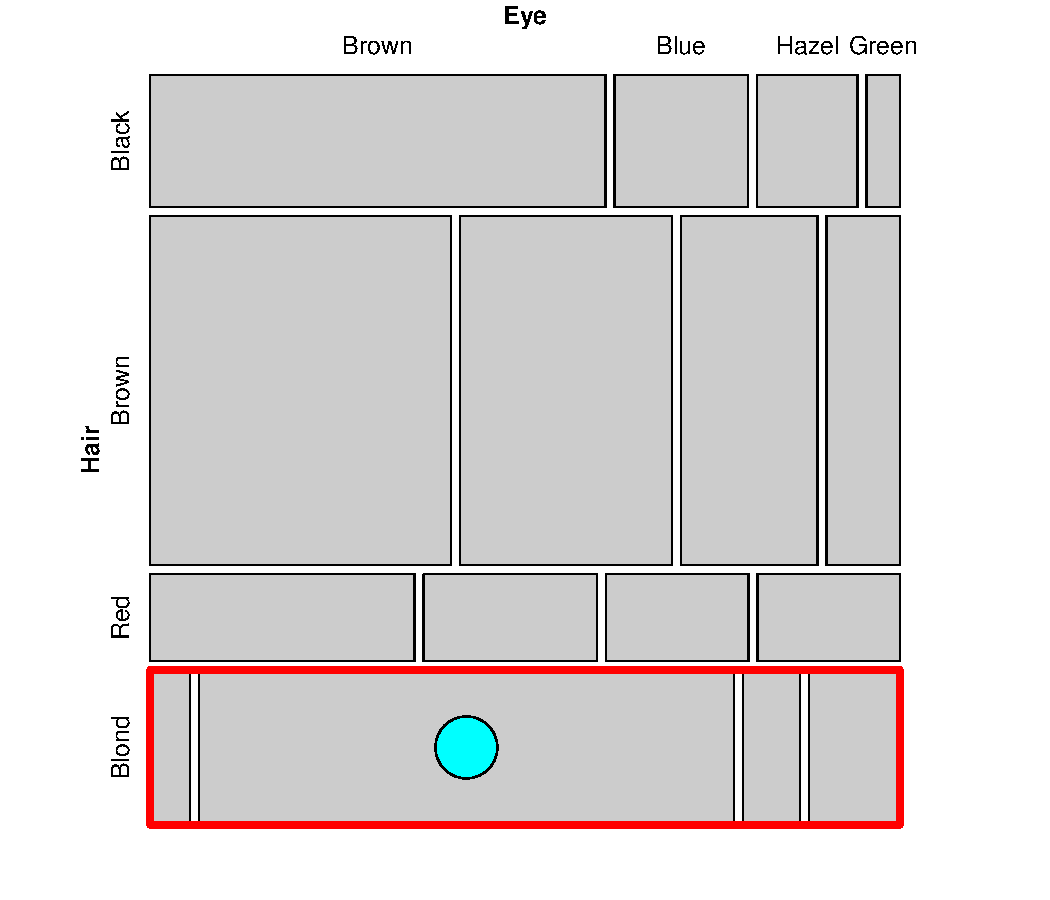
\includegraphics{strucplot-viewportnamesfig}
\caption{Adding elements to a mosaic plot after drawing.}
\label{fig:afterplot}
\end{center}
\end{figure}

In addition to the viewports, the main graphical elements get names
following a similar construction method. This allows to change
graphical parameters of plot elements \emph{after} 
the plotting (see Figure~\ref{fig:changeplot}):

\begin{Schunk}
\begin{Sinput}
> assoc(Eye ~ Hair, data = HEC, pop = FALSE)
> getNames()[1:6]
\end{Sinput}
\begin{Soutput}
[1] "GRID.lines.2729"           "rect:Hair=Black,Eye=Brown"
[3] "GRID.lines.2730"           "rect:Hair=Black,Eye=Blue" 
[5] "GRID.lines.2731"           "rect:Hair=Black,Eye=Hazel"
\end{Soutput}
\begin{Sinput}
> grid.edit("rect:Hair=Blond,Eye=Blue", gp = gpar(fill = "red"))
\end{Sinput}
\end{Schunk}

%% code-chunk reuse does not work with parameter changing
\begin{figure}[h]
\begin{center}
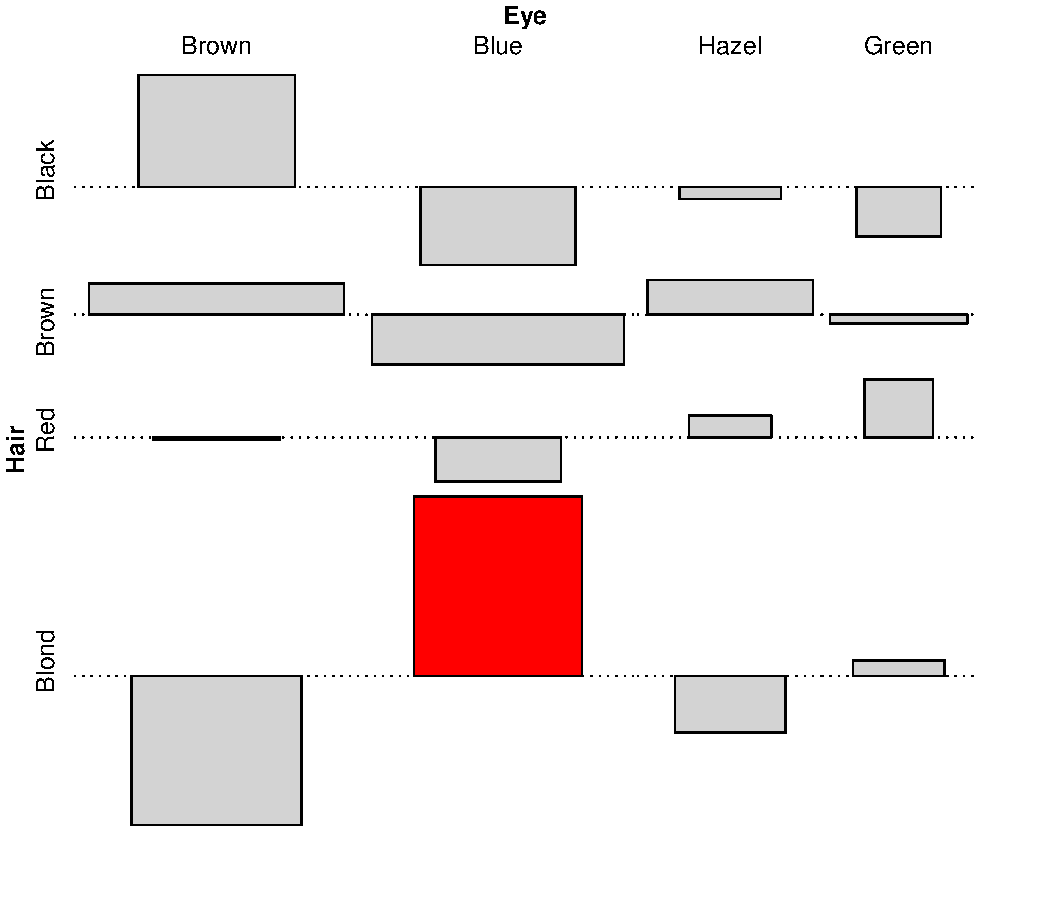
\includegraphics{strucplot-changeplotfig}
\caption{Changing graphical parameters of elements after drawing.}
\label{fig:changeplot}
\end{center}
\end{figure}

\subsection{Performance issues}
\label{sec:performance}

As stated above, the implementation of strucplot displays is based on
creating and nesting \pkg{grid} viewports. The main time-consuming steps performed by
the core functions are the following:

\begin{enumerate}
\item recursively, split the table until the individual cells are reached
\item during the splits, add viewports to the plot
\item for the individual cells, add plot-specific content 
      (rectangles for mosaics, bars for association plots, etc.)
\end{enumerate}

\noindent All these operations scale linearly with the amount of
created viewports. For a $d$-dimensional table with $k_i$
levels, $i=1 \dots d$, the total number of needed viewports
$T_d$ can roughly be estimated as

\begin{equation}
  \label{eq:numbervp}
  T_d \quad = \quad k_1 + k_1k_2 + \cdots + k_1 \cdots k_d \quad =\quad \sum_{i=1}^d \prod_{j \le i} k_j
\end{equation}

\noindent since we first push the $k_1$ viewports for the levels of the
first dimension, then, for \emph{each} of these, the $k_2$ levels of
the second dimension, etc. If the number of levels is equal ($k$) for
all dimensions, $T_d$ simplifies to

\begin{equation}
  \label{eq:equalvp}
  T_d \quad = \quad \sum_{i=1}^d k^i = \frac{k(k^d-1)}{k-1}
\end{equation}

\noindent and so the time complexity for drawing a strucplot display is of order $k^d$.

\section{Shadings}
\label{sec:shading}


Unlike other graphics functions in base \proglang{R}, the strucplot framework 
allows almost full control over the graphical parameters of all plot elements. In
particular, in association plots, mosaic plots, and sieve plots, 
the user can modify the graphical appearance of each tile individually. 
Built on top of this functionality, the
framework supplies a set of shading functions choosing colors
appropriate for the visualization of log-linear models.
The tiles' graphical parameters are set using the \code{gp} argument
of the functions of the strucplot framework. This argument basically expects an object
of class \class{gpar} whose components are arrays of the same shape 
(length and dimensionality) as the data table (see Section \ref{sec:gp}). 
For convenience, however, the user can also
supply a grapcon function that computes such an object given a vector of
residuals, or, alternatively, a generating function that takes
certain arguments and returns such a grapcon function (see Section
\ref{sec:shadingcustom}). We provide several shading functions, including
support for both HSV and HCL colors, and the
visualization of significance tests (see Section \ref{sec:overview}).

\subsection{Specifying graphical parameters of strucplot displays}
\label{sec:gp}

As an example, consider the \data{UCBAdmissions} data. 
In the table aggregated over departments, we
would like to highlight the (incidentally wrong) impression that there
were too many male students accepted compared to the presumably
discriminated female students (see Figure~\ref{fig:ucb}):

\begin{Schunk}
\begin{Sinput}
> (ucb <- margin.table(UCBAdmissions, 1:2))
\end{Sinput}
\begin{Soutput}
          Gender
Admit      Male Female
  Admitted 1198    557
  Rejected 1493   1278
\end{Soutput}
\begin{Sinput}
> (fill_colors <- matrix(c("dark cyan", "gray", "gray", 
+     "dark magenta"), ncol = 2))
\end{Sinput}
\begin{Soutput}
     [,1]        [,2]          
[1,] "dark cyan" "gray"        
[2,] "gray"      "dark magenta"
\end{Soutput}
\begin{Sinput}
> mosaic(ucb, gp = gpar(fill = fill_colors, col = 0))
\end{Sinput}
\end{Schunk}

\begin{figure}[h]
\begin{center}
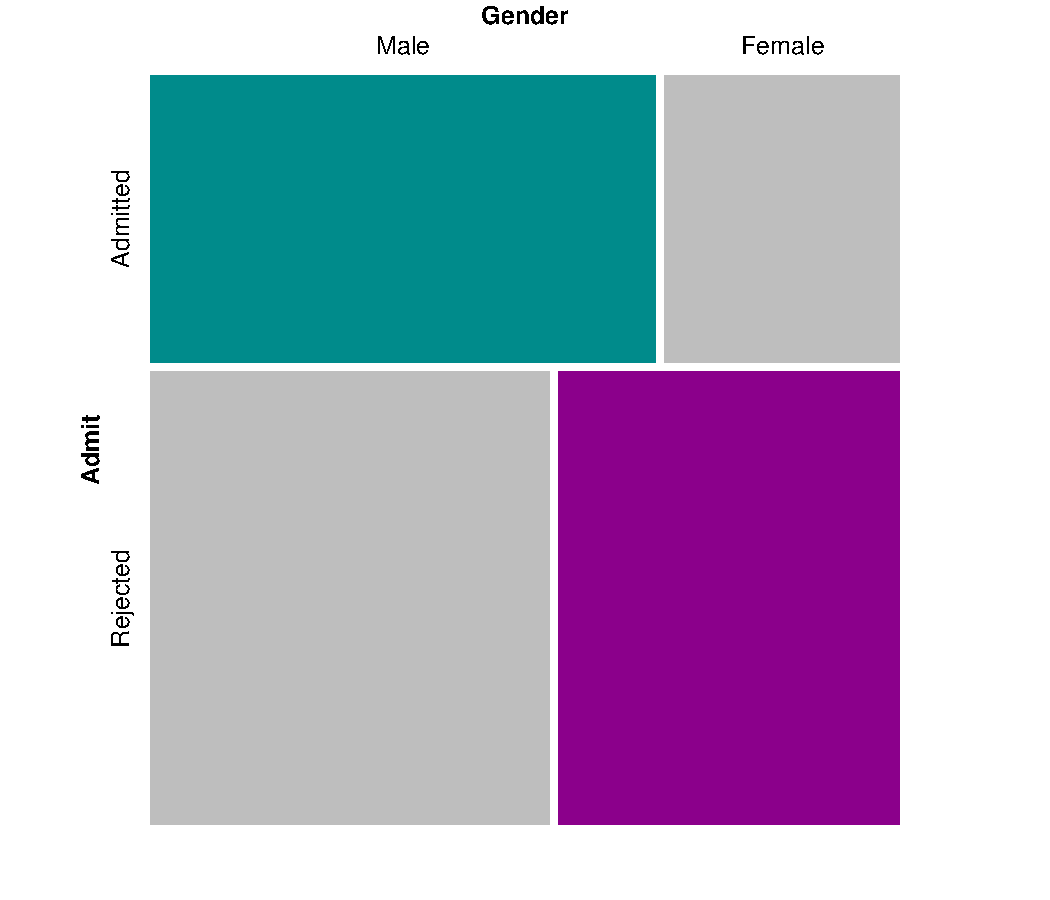
\includegraphics{strucplot-ucbfig}

\caption{Mosaic plot for the \data{UCBAdmissions} data with highlighted cells.}
\label{fig:ucb}
\end{center}
\end{figure}

\noindent As the example shows, we create a fourfold table 
with appropriate colors (dark cyan for admitted male students and dark
magenta for rejected female students) and supply them to the \code{fill} component 
of the \class{gpar} object passed to the \code{gp} argument of \codefun{mosaic}. 
For visual clarity, we additionally hide the tiles' borders by setting the \code{col} 
component to 0 (transparent).

If the parameters specified in the \class{gpar} object are ``incomplete'',
they will be recycled along the last splitting
dimension. In the following example based on the \data{Titanic} data, 
we will highlight all cells corresponding to survived
passengers (see Figure~\ref{fig:recycling}):

\begin{Schunk}
\begin{Sinput}
> mosaic(Titanic, gp = gpar(fill = c("gray", "dark magenta")), 
+     spacing = spacing_highlighting, labeling_args = list(abbreviate = c(Age = 3), 
+         rep = c(Survived = FALSE)))
\end{Sinput}
\end{Schunk}

\noindent Note that \codefun{spacing\_highlighting} sets the spaces
between tiles in the last dimension to 0. The \code{labeling\_args} 
argument ensures that labels do not overlap (see Section \ref{sec:labeling}).

\begin{figure}[h]
\begin{center}
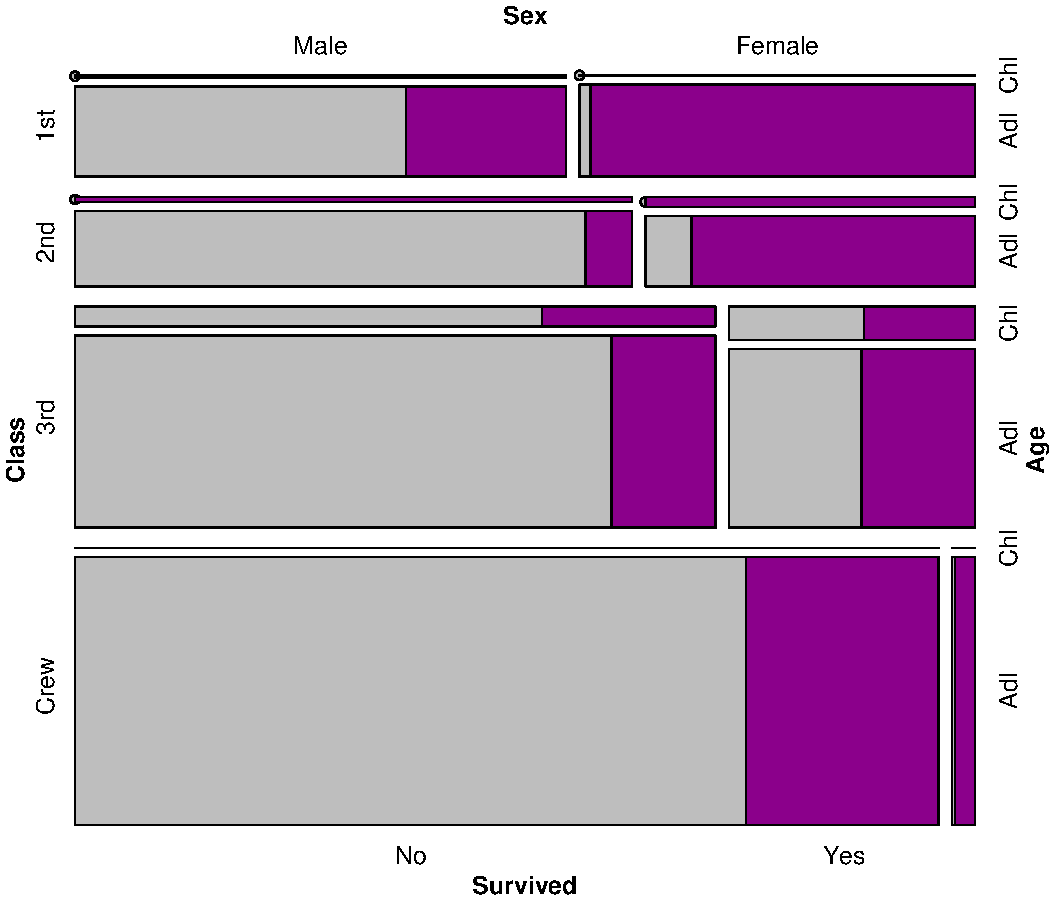
\includegraphics{strucplot-recyclingfig}
\caption{Recycling of parameters, used for highlighting the survived
  passengers in the \data{Titanic} data.}
\label{fig:recycling}
\end{center}
\end{figure}

\subsection{Customizing residual-based shadings}
\label{sec:shadingcustom}

This flexible way of specifying graphical parameters is the basis for a suite of
shading functions that modify the tiles' appearance with respect to a vector of 
residuals, resulting from deviations of observed from expected
frequencies under a given log-linear model. 
The idea is to visualize at least sign and absolute size of the residuals, but some
shadings, additionally, indicate overall significance. One particular
shading, the maximum shading 
\citep{vcd:Meyer+Zeileis+Hornik:2003,vcd:Zeileis+Meyer+Hornik:2005},
even allows to identify the cells that cause the rejection of the null hypothesis.

Conceptually, the strucplot framework offers three alternatives to
add residual-based shading to plots:

\begin{enumerate}
\item Precomputing the graphical parameters (e.g., fill colors),
  encapsulating them into an object of class
  \class{gpar} as demonstrated in the previous section, and
  passing this object to the \code{gp} argument.
\item Providing a grapcon function to the \code{gp} argument that 
  takes residuals as input and returns an object as described in
  alternative 1.
 \item Providing a grapcon generator taking parameters and 
   returning a function as described in alternative~2.
\end{enumerate}

\noindent For each of these approaches, we will demonstrate the
necessary steps to obtain a binary shading that visualizes the sign of
the residuals by a corresponding 
fill color (for simplicity, we will treat 0 as positive).

\subsubsection*{Alternative 1: Precomputed \class{gpar} object}

The first method is precomputing the graphical parameters ``by
hand''. We will use \code{royalblue4} color for positive and \code{mediumorchid4}
color for negative residuals (see Figure~\ref{fig:binary}):

\begin{Schunk}
\begin{Sinput}
> expected <- independence_table(ucb)
> (x <- (ucb - expected)/sqrt(expected))
\end{Sinput}
\begin{Soutput}
          Gender
Admit           Male    Female
  Admitted  4.784093 -5.793466
  Rejected -3.807325  4.610614
\end{Soutput}
\begin{Sinput}
> (shading1_obj <- ifelse(x > 0, "royalblue4", "mediumorchid4"))
\end{Sinput}
\begin{Soutput}
          Gender
Admit      Male            Female         
  Admitted "royalblue4"    "mediumorchid4"
  Rejected "mediumorchid4" "royalblue4"   
\end{Soutput}
\begin{Sinput}
> mosaic(ucb, gp = gpar(fill = shading1_obj))
\end{Sinput}
\end{Schunk}

\begin{figure}[h]
\begin{center}
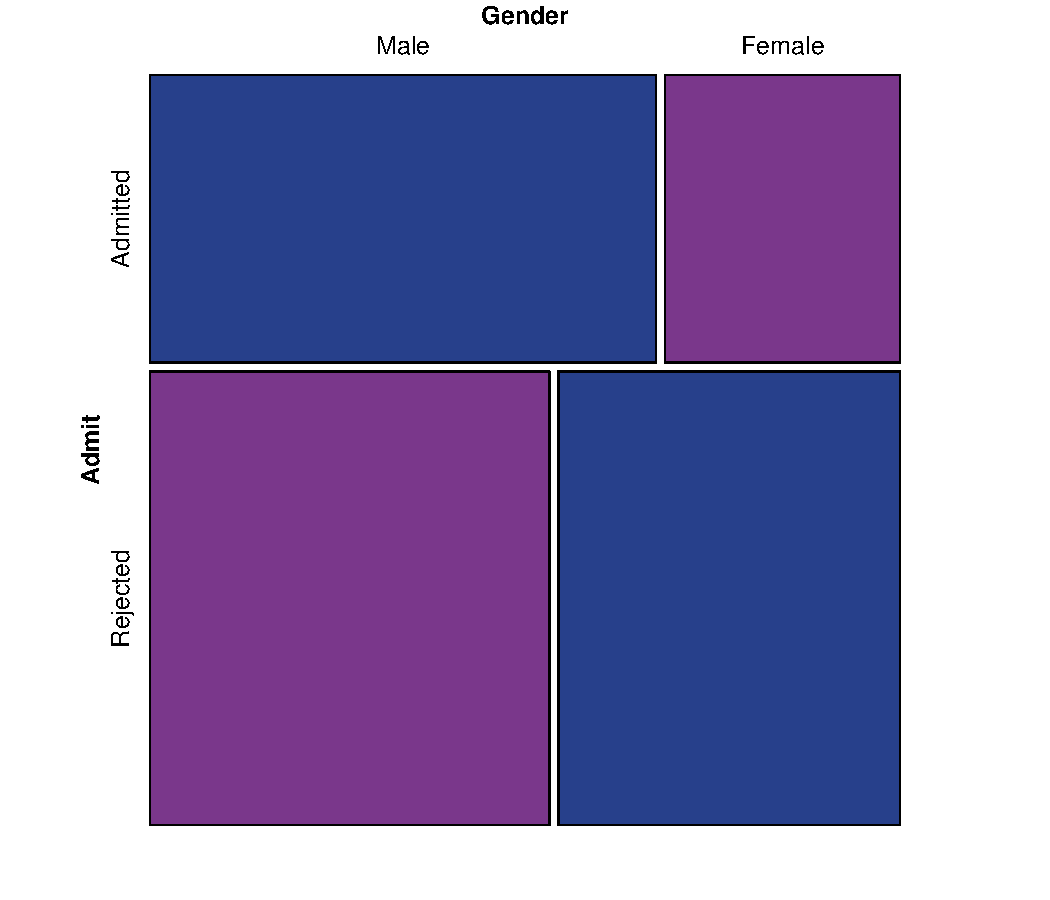
\includegraphics{strucplot-shading1fig}
\caption{Binary shading visualizing the sign of the residuals.}
\label{fig:binary}
\end{center}
\end{figure}

\subsubsection*{Alternative 2: Grapcon function}

For implementing alternative 2, we need to create a ``shading function''
that computes \class{gpar} objects from
residuals. For that, we can just reuse the code from the previous step:

\begin{Schunk}
\begin{Sinput}
> shading2_fun <- function(x) gpar(fill = ifelse(x > 0, 
+     "royalblue4", "mediumorchid4"))
\end{Sinput}
\end{Schunk}

\noindent To create a mosaic display with binary shading, 
it now suffices to specify the data table along with
\codefun{shading2\_fun}:

\begin{Schunk}
\begin{Sinput}
> mosaic(ucb, gp = shading2_fun)
\end{Sinput}
\end{Schunk}

\noindent \codefun{mosaic} internally calls
\codefun{strucplot} which computes the residuals from the specified
independence model (total independence by default), passes them to
\codefun{shading2\_fun}, and uses the \class{gpar} object returned 
to finally create the plot.

Our \codefun{shading2\_fun} function might be useful, 
but can still be improved: the hard-wired colors should be
customizable. We cannot
simply extend the argument list to include, e.g., 
a \code{fill = c("royalblue4", "mediumorchid4")} argument because
\codefun{strucplot} will neither know how to handle it, nor let us
change the defaults. In fact, the interface of shading functions is fixed,
they are expected to take exactly one argument: a table of residuals. 
This is where generating functions (alternative 3) come
into play. 

\subsubsection*{Alternative 3: Grapcon generator}

We simply wrap our grapcon shading function in another 
function that takes all additional arguments it needs to use, possibly
preprocesses them, and returns the actual shading function. This returned
function will have access to the parameters since in \proglang{R}, nested
functions are lexically scoped. Thus, the grapcon generator
returns (``creates'') a 
``parameterized'' shading function with the minimal standard interface
\codefun{strucplot} requires. The following example shows the necessary
extensions for our running example:

\begin{Schunk}
\begin{Sinput}
> shading3a_fun <- function(col = c("royalblue4", "mediumorchid4")) {
+     col <- rep(col, length.out = 2)
+     function(x) gpar(fill = ifelse(x > 0, col[1], col[2]))
+ }
\end{Sinput}
\end{Schunk}

\noindent The first statement just makes sure that exactly two colors
are specified. In the call to \codefun{mosaic}, using the new
\codefun{shading3a\_fun} function, we can now simply change the colors:

\begin{Schunk}
\begin{Sinput}
> mosaic(ucb, gp = shading3a_fun(c("royalblue4", "mediumorchid4")))
\end{Sinput}
\end{Schunk}

\noindent (figure not shown).  The procedure described so far is a
rather general concept, applicable to a wide family of user-level
\pkg{grid} graphics. Indeed, the customization of other components of
the strucplot framework (labeling, spacing, legend, and core functions)
follows the same idea.  Now for the shading functions, more
customization is needed. Note that \codefun{shading3a\_fun} needs to be
evaluated by the user, even if the defaults are to be used. It is a
better idea to let \codefun{strucplot} call the generating function,
which, in particular, allows the passing of arguments that are computed
by \codefun{strucplot}. Since shading functions can be used for
visualizing significance (see Section \ref{sec:overview}), it makes
sense for generating functions to have access to the model, i.e.,
observed and expected values, residuals, and degrees of freedom. For
example, the \codefun{shading\_max} generating function computes a
permutation distribution of the maximum statistic and $p$ values for
specified significance levels based on the observed table to create
data-driven cut-off points. If this was done in the shading function
itself, the permutation statistic would be recomputed every time the
shading function is called, resulting in possibly severe performance
loss and numerical inconsistencies. Therefore, generating functions for
shadings are required to take at least the parameters \code{observed},
\code{expected}, \code{residuals}, and \code{df} (these are provided by
the strucplot framework), followed by other parameters controlling the
shading appearance (to be specified by the user):

\begin{Schunk}
\begin{Sinput}
> shading3b_fun <- function(observed = NULL, residuals = NULL, 
+     expected = NULL, df = NULL, col = c("royalblue4", 
+         "mediumorchid4")) {
+     col <- rep(col, length.out = 2)
+     function(x) gpar(fill = ifelse(x > 0, col[1], col[2]))
+ }
> class(shading3b_fun) <- "grapcon_generator"
\end{Sinput}
\end{Schunk}

Note that in this simple binary shading example, the first four
parameters are not used. In some sense, generating
functions for shadings are parameterized both by the user and the
strucplot framework. For shading functions that require model
information, the user-specified parameters are 
to be passed to the \code{gp\_args} argument instead, and for this to
work, the generating function needs a class attribute to be distinguishable from
the ``normal'' shading functions. For others
(like our simple \codefun{shading3b\_fun}) this is optional, but
recommended for consistency:

\begin{Schunk}
\begin{Sinput}
> mosaic(ucb, gp = shading3b_fun, gp_args = list(col = c("red", 
+     "blue")))
\end{Sinput}
\end{Schunk}

\noindent The final \codefun{shading3b\_fun} pretty much resembles 
\codefun{shading\_binary}, one of the standard shading
functions provided by the \pkg{vcd} package.

\subsection[An overview of the shading functions in vcd]{An overview of the shading functions in \pkg{vcd}}
\label{sec:overview}

\cite{vcd:Friendly:1994}
suggested a residual-based shading for the mosaic tiles that can also be applied
to the rectangles in association plots \citep{vcd:Meyer+Zeileis+Hornik:2003}.
Apart from \codefun{shading\_binary}, there are currently two basic
shadings available in \pkg{vcd}:
\codefun{shading\_hcl} and \codefun{shading\_hsv}, as well
as two derived functions: \codefun{shading\_Friendly} building upon
\codefun{shading\_hsv}, and \codefun{shading\_max} building upon \codefun{shading\_hcl}.
\codefun{shading\_hsv} and \codefun{shading\_hcl} provide
the same conceptual tools, but use different color spaces: the
Hue-Saturation-Value (HSV) and the Hue-Chroma-Luminance (HCL) scheme,
respectively. We will first expose the basic concept of these shading
functions using HSV space, and
then briefly explain the differences to HCL space \citep[a detailed
discussion can be found in][]{vcd:Zeileis+Meyer+Hornik:2005}. 
Color palettes in HCL space are 
preferable to palettes derived 
from HSV space from a perceptual point of view. Functions for creating
palettes (see, e.g., \codefun{diverge\_hcl}) are provided with the
\pkg{vcd} package.

In HSV space, colors are specified in three dimensions: Hue,
Saturation (``colorfulness''), and Value (``lightness'', amount of gray). 
These three dimensions are used by \codefun{shading\_hsv} to visualize information 
about the residuals and the underlying independence model. The hue 
indicates the residuals' sign: by default, blue for positive, and red
for negative residuals. The saturation of a residual 
is set according to its size: high saturation for large, and low
saturation for small residuals. 
Finally, the overall lightness is used to indicate the significance of
a test statistic: light colors for significant, 
and dark colors for non-significant results. 

As an example, we will visualize the association of hair and eye
color in the \data{HairEyeColor} data set (see
Figure~\ref{fig:haireye}, top):

\begin{Schunk}
\begin{Sinput}
> haireye <- margin.table(HairEyeColor, 1:2)
> mosaic(haireye, gp = shading_hsv)
\end{Sinput}
\end{Schunk}

\noindent As introduced before, the default shading scheme is not
\codefun{shading\_hsv} but \codefun{shading\_hcl} due to the better
perceptual characteristics of HCL color space.
The following example again illustrates the \data{HairEyeColor} data, 
this time with HCL colors: 

\begin{Schunk}
\begin{Sinput}
> mosaic(haireye, gp = shading_hcl)
\end{Sinput}
\end{Schunk}
\begin{Schunk}
\begin{Sinput}
> mosaic(haireye, gp = shading_hcl, gp_args = list(h = c(130, 
+     43), c = 100, l = c(90, 70)))
\end{Sinput}
\end{Schunk}

\noindent In Figure~\ref{fig:haireye}, the plot
in the middle depicts the default palette, 
and the bottom plot an alternative setting for Hue (\code{h}), Chroma (\code{c}), and
Luminance (\code{l}).

\setkeys{Gin}{width=0.5\textwidth}
\begin{figure}[htbp]
\begin{center}
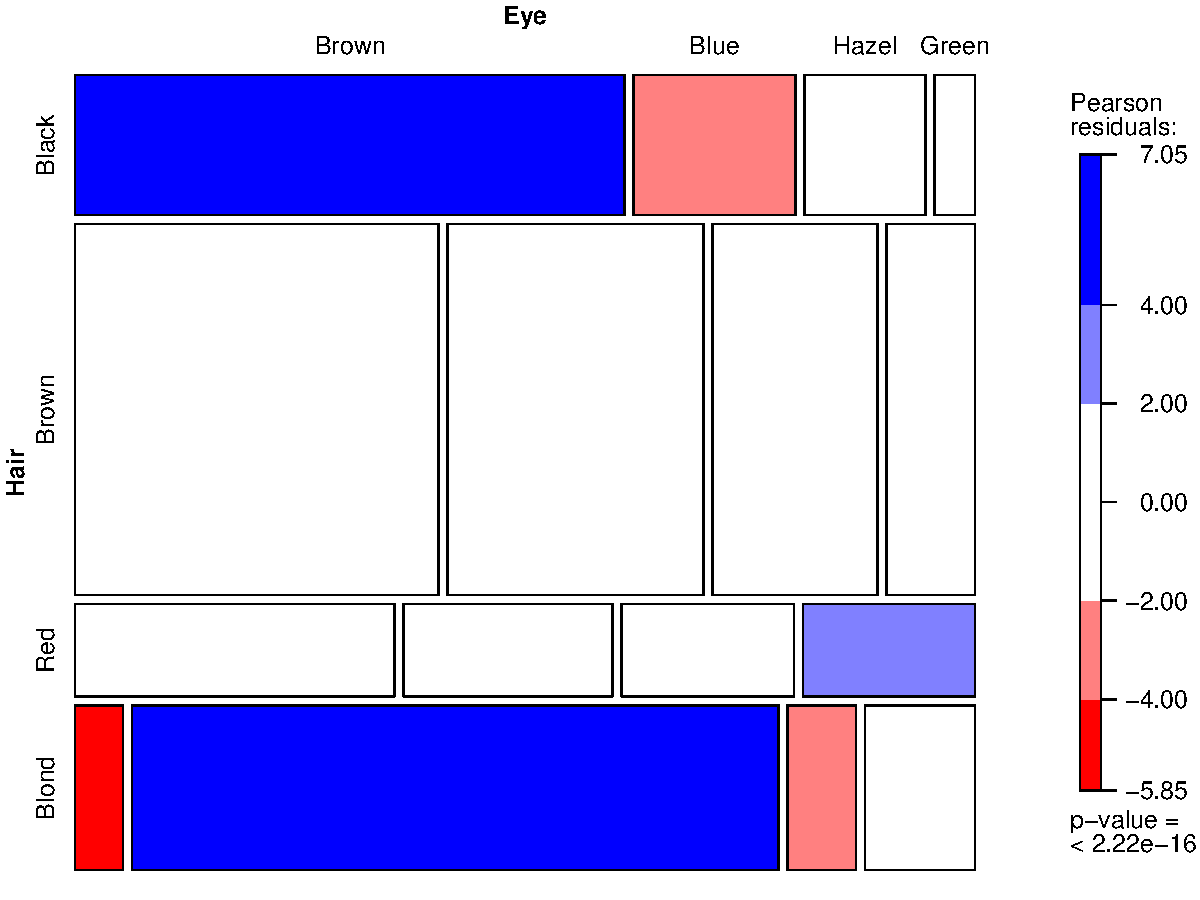
\includegraphics{strucplot-haireyefig1}
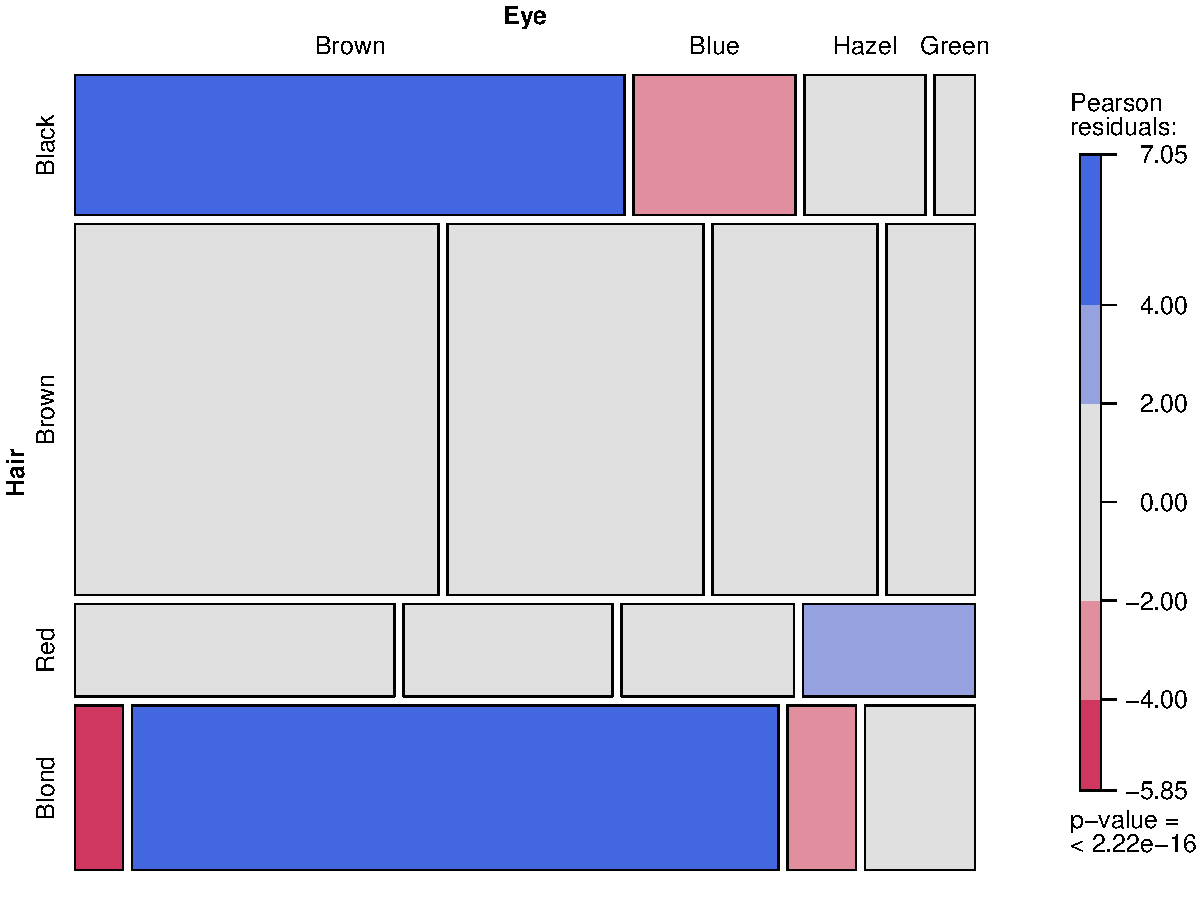
\includegraphics{strucplot-haireyefig2}
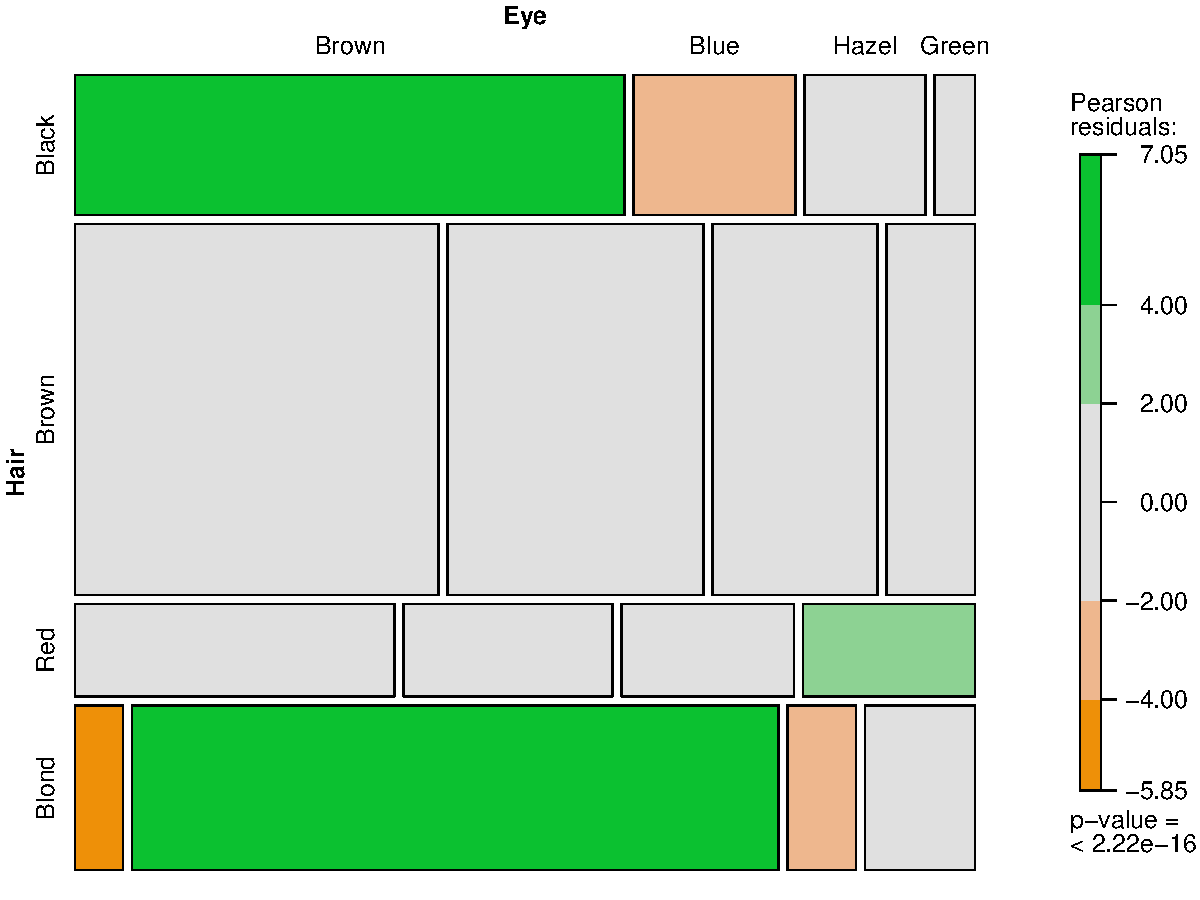
\includegraphics{strucplot-haireyefig3}
\caption{Three mosaic plots for the \data{HairEyeColor} data using
  different color palettes. Top: default HSV color palette. Middle: default HCL
 color palette. Bottom: a custom HCL color palette.}
\label{fig:haireye}
\end{center}
\end{figure}
\setkeys{Gin}{width=0.7\textwidth}

\noindent Large positive residuals (greater than $4$) can be found for
brown eyes/black hair and blue eyes/blond hair, and are colored in deep blue. 
On the other hand, there is a large negative residual
(less than $-4$) for brown eyes/blond hair, colored deep red. There are also three
medium-sized positive (negative) residuals between 2 and 4 ($-2$ and
$-4$): the colors for them are less saturated. Residuals between $-2$ and $2$ 
are shaded in white (gray for HCL-shading).
The heuristic for choosing the cut-off points $2$ and $4$ is that the Pearson residuals
are approximately standard normal which implies that the highlighted cells are those with
residuals \emph{individually} significant at approximately the $\alpha
= 0.05$ and $\alpha = 0.0001$ levels, respectively. These default cut-off points can
be changed to alternative values using the \code{interpolate}
argument (see Figure~\ref{fig:interpolatecontinuous}):

\begin{Schunk}
\begin{Sinput}
> mosaic(haireye, shade = TRUE, gp_args = list(interpolate = 1:4))
\end{Sinput}
\end{Schunk}

\noindent The elements of the numeric vector passed to
\code{interpolate} define the knots of an interpolating step function
used to map the absolute residuals to saturation levels. 
The \code{interpolate} argument also accepts a user-defined function,
which then is called with the absolute residuals to get a vector of
cut-off points. Thus, it is possible to automatically choose the cut-off points 
in a data-driven way. For example,
one might think that the extension from four cut-off points 
to a continuous shading---visualizing the whole range of 
residuals---could be useful. We simply need a one-to-one
mapping from the residuals to the saturation values: 

\begin{Schunk}
\begin{Sinput}
> ipol <- function(x) pmin(x/4, 1)
\end{Sinput}
\end{Schunk}

\noindent Note that this \codefun{ipol} 
function maps residuals greater than 4 to a saturation
level of 1. However, the resulting plot
(Figure~\ref{fig:interpolatecontinuous}, right) is 
deceiving: 

\begin{Schunk}
\begin{Sinput}
> mosaic(haireye, shade = TRUE, gp_args = list(interpolate = ipol), 
+     labeling_args = list(abbreviate = c(Sex = TRUE)))
\end{Sinput}
\end{Schunk}

\setkeys{Gin}{width=\textwidth}
\begin{figure}[htbp]
\begin{center}
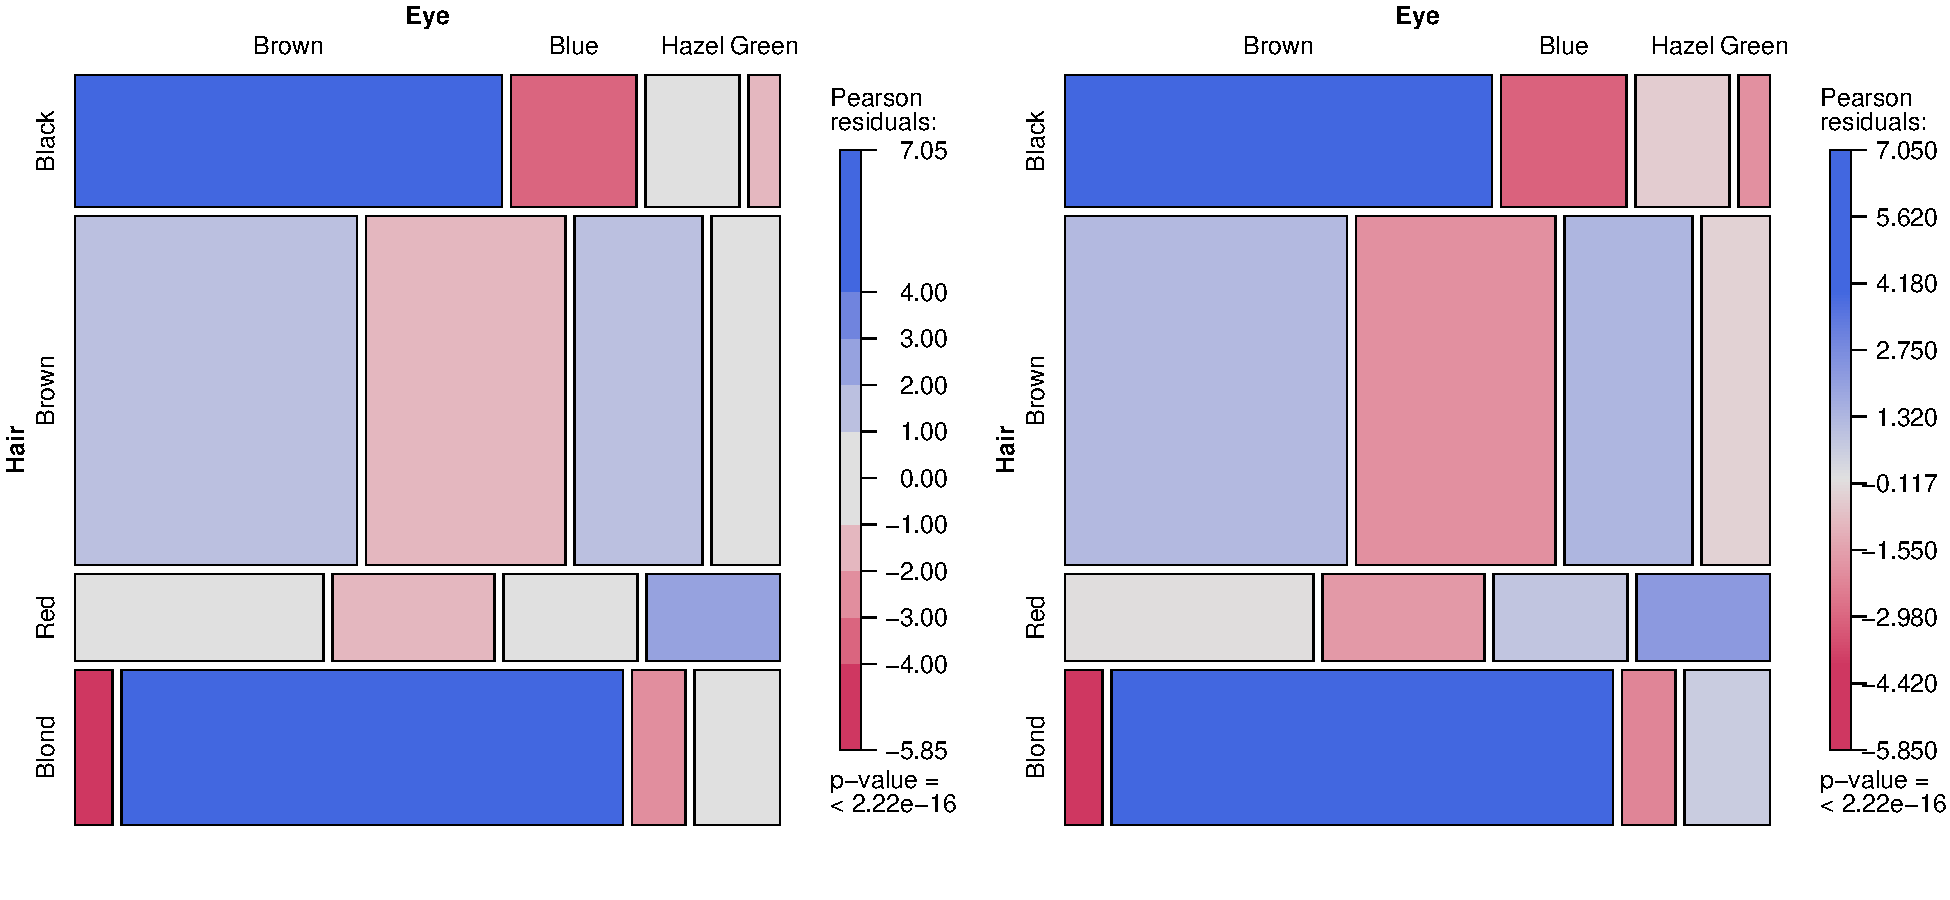
\includegraphics{strucplot-interpolatefig}
\caption{\label{fig:interpolatecontinuous}The \data{HairEyeColor}
  data. Left: shading with 4 cut-off points. Right: continuous shading.}

\end{center}
\end{figure} 
\setkeys{Gin}{width=0.7\textwidth}

\noindent Too much color makes it difficult to interpret the image, and the subtle color
differences are hard to catch. Therefore, we only included shadings
with discrete cut-off points.

The third remaining dimension, the value, is used for
visualizing the significance of a test statistic. The user can either
directly specify the $p$ value, or, alternatively, a function that
computes it, to the \code{p.value} argument. Such a function must take
observed and expected values, residuals, and degrees of freedom (used
by the independence model) as arguments. 
If nothing is specified, the $p$ value is computed from 
a $\chi^2$ distribution with \code{df} degrees of
freedom. The \code{level} argument is used to specify the confidence
level:  if \code{p.value} is smaller than \code{1 - level}, light colors are used, 
otherwise dark colors are employed. 
The following example using the \data{Bundesliga} data 
shows the relationship of home goals and away
goals of Germany's premier soccer league in 1995: although there are two
``larger'' residuals (one greater than 2, one less then $-2$), the
$\chi^2$ test does not reject the null hypothesis of
independence. Consequently, the colors appear dark (see
Figure~\ref{fig:bundesliga}, left):

\begin{Schunk}
\begin{Sinput}
> BL <- xtabs(~HomeGoals + AwayGoals, data = Bundesliga, 
+     subset = Year == 1995)
> mosaic(BL, shade = TRUE)
\end{Sinput}
\end{Schunk}

\noindent Note that in extended mosaic plots, bullets drawn for zero
cells are shaded, too, bringing out non-zero residuals, if any. 

A shading function building upon \codefun{shading\_hsv} is \codefun{shading\_Friendly},
implementing the shading introduced by \cite{vcd:Friendly:1994}. In addition
to the defaults of the HSV shading, it uses the border color and line type to 
redundantly code the residuals' sign. The following example again uses 
the \data{Bundesliga} data from above, this time using the Friendly 
scheme and, in addition, an alternative legend (see
Figure~\ref{fig:bundesliga}, right):

\begin{Schunk}
\begin{Sinput}
> mosaic(BL, gp = shading_Friendly, legend = legend_fixed, 
+     zero_size = 0)
\end{Sinput}
\end{Schunk}

\setkeys{Gin}{width=\textwidth}
\begin{figure}[htbp]
\begin{center}
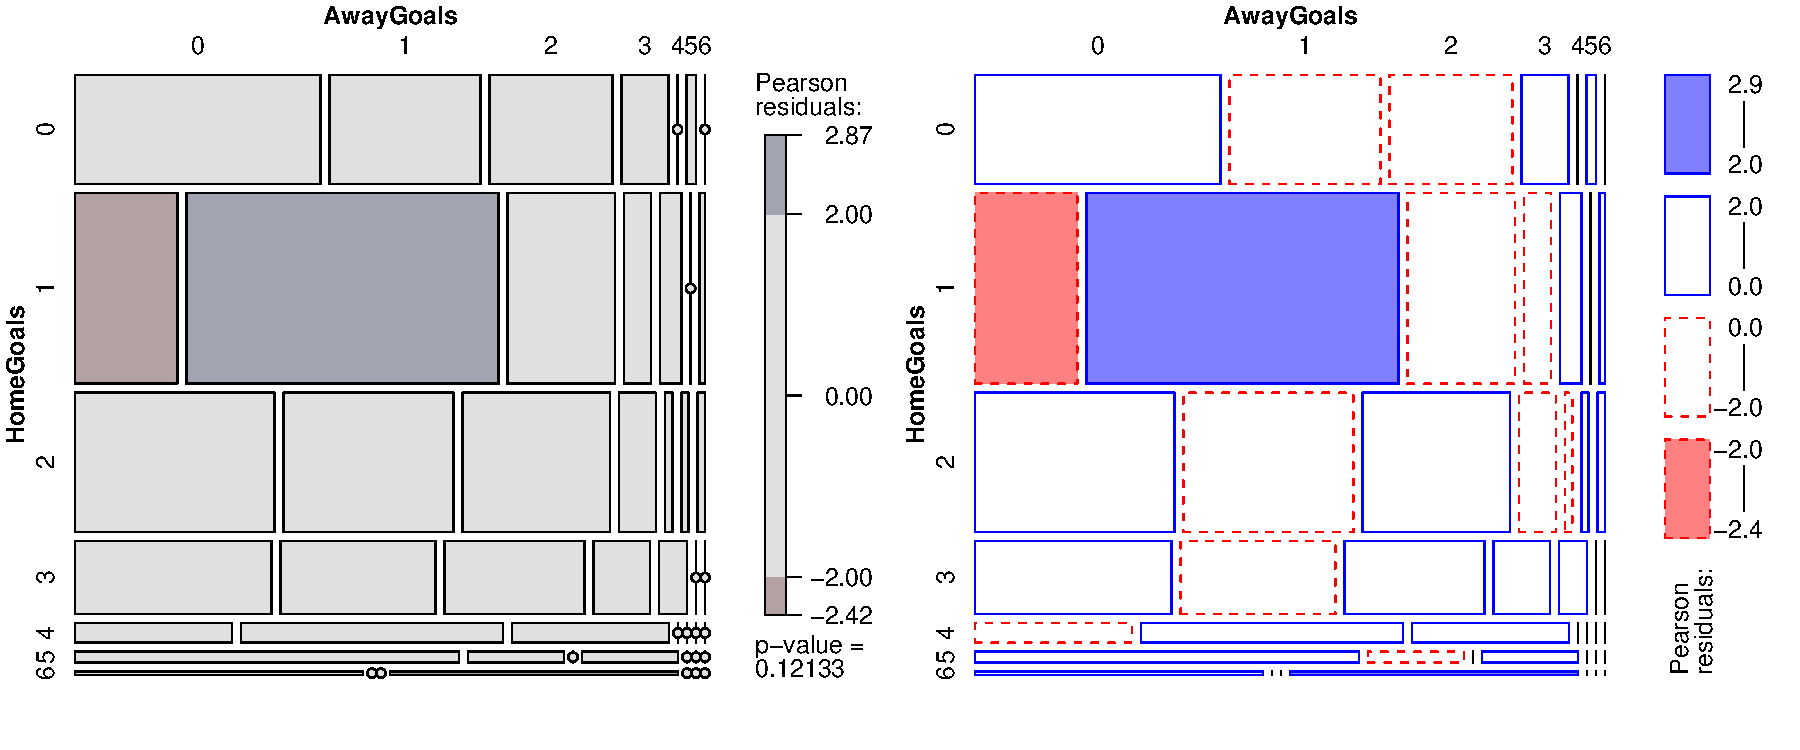
\includegraphics{strucplot-bundesligafig}
\caption{The \data{Bundesliga} data for 1995. Left: Non-significant
  $\chi^2$ test. Right: using the Friendly
  shading and a legend with fixed bins.}
\label{fig:bundesliga}
\end{center}
\end{figure}
\setkeys{Gin}{width=0.7\textwidth}

\noindent (The \code{zero\_size = 0} argument removes the bullets indicating zero 
observed values. This feature is not provided
in the original \proglang{SAS} implementation of the Friendly mosaic plots.)

% Figure~\ref{fig:shadingHSVHCL} depicts 
% HSV space in the upper panel and HCL space in the lower panel.
% On the left (right) side, we see the color scales for red (blue)
% hue, respectively. The $x$-axis represents the colorfulness, and the
% $y$-axis the brightness.
% The boxes represent the diverging color palettes used for the shadings.
% For HSV space, we can see that the effect of changing the 
% level of brightness (`value') is not the same for different levels of 
% saturation, and again not the same for the two different hues.
% In fact, in HSV space all dimensions are confounded, which 
% obviously is problematic for coding information. In contrast, HCL color
% space offers perceptually uniform colors: as can be seen from the lower panel, 
% the chroma is homogeneous for different levels of luminance. 
% Unfortunately, this comes at the 
% price of the space being irregularly shaped, making it difficult to automatically select 
% diverging color palettes. 
% <<auxiliary_functions,echo=FALSE,results=hide>>=
% hue.slice <- function(hue, grid.n = 101, type = c("HCL", "HSV"), plot = TRUE, fixup = FALSE)
% {
%   type <- match.arg(type)
%   if(type == "HCL") {
%     chroma = seq(0, 100, length = grid.n)
%     luminance = seq(0, 100, length = grid.n)
%     nc <- length(chroma)
%     nl <- length(luminance)
%     color.slice <- outer(chroma, luminance, function(y, x) hcl(hue, x, y, fixup = fixup))
%     xlab <- "chroma"
%     ylab <- "luminance"
%     main <- paste("hue =", round(hue, digits = 0))
%   } else {
%     chroma = seq(0, 1, length = grid.n)
%     luminance = seq(0, 1, length = grid.n)
%     nc <- length(chroma)
%     nl <- length(luminance)
%     color.slice <- outer(chroma, luminance, function(y, x) hsv(hue, x, y))
%     xlab <- "saturation"
%     ylab <- "value"
%     main <- paste("hue =", round(hue, digits = 3))
%   }
%   if(plot) {
%     plot(0.5, 0.5, xlim = range(chroma), ylim = range(luminance), type = "n", axes = FALSE,
%          xlab = xlab, ylab = ylab, yaxs = "i", xaxs = "i", main = main)
%     for(i in 1:(nc-1)) {
%       rect(chroma[i], luminance[-nl], chroma[i] + 100/(nc-1), luminance[-1], border = color.slice[,i+1], col = color.slice[,i+1])
%     }
%     axis(1)
%     axis(2)
%     box()
%   }
%   colnames(color.slice) <- chroma
%   rownames(color.slice) <- luminance
%   attr(color.slice, "type") <- type
%   class(color.slice) <- "slice"
%   invisible(color.slice)
% }
% @

% \setkeys{Gin}{width=.8\textwidth}
% \begin{figure}[p]
% \begin{center}
% <<shading_HSV,fig=TRUE,echo=FALSE,height=7,width=8>>=
% ## generate colors
% hue23 <- hue.slice(2/3, grid.n = 101, plot = FALSE, type = "HSV")
% hue0 <- hue.slice(0, grid.n = 101, plot = FALSE, type = "HSV")
% saturation <- as.numeric(colnames(hue23))
% value <- as.numeric(rownames(hue23))

% ## select those with value >= 0.5
% hue23 <- hue23[value >= .5, ]
% hue0 <- hue0[value >= .5, ]
% value <- value[value >= .5]
% nl <- nrow(hue23)
% nc <- ncol(hue23)

% ## plot 2 slides from HSV space
% plot(0.5, 0.5, xlim = c(-1, 1), ylim = c(0, 1), type = "n", axes = FALSE,
%        xlab = "", ylab = "", yaxs = "i", xaxs = "i", main = "")
% for(i in 1:(nc-1)) {
%   rect(saturation[i], value[-nl], saturation[i] + 1/(nc-1), value[-1], border = hue23[,i+1], col = hue23[,i+1])
% }
% for(i in 1:(nc-1)) {
%   rect(-saturation[i], value[-nl], -(saturation[i] + 1/(nc-1)), value[-1], border = hue0[,i+1], col = hue0[,i+1])
% }
% axis(2, at = c(50, 75, 100)/100, labels = c(0.5, 0.75, 1))
% axis(4, at = c(50, 75, 100)/100, labels = c(0.5, 0.75, 1))
% axis(3, at = -4:4*.25, labels=c(4:0*.25, 1:4*.25))
% mtext(c("hue = 0", "hue = 2/3"), side = 3, at = c(-.5, .5), line = 3, cex = 1.2)
% mtext("saturation", side = 3, at = 0, line = 2)
% mtext("value", side = 2, at = .75, line = 2)
% mtext("value", side = 4, at = .75, line = 2)
% lines(c(-1, 1), c(.5, .5))

% ## significant colors
% rect(-1, 0.95, -.90, 1, col = hsv(0, 1, 1))
% rect(-0.45, 0.95, -.55, 1, col = hsv(0, 0.5, 1))
% rect(-.05, .95, .05, 1, col = hsv(2/3, 0, 1))
% rect(0.45, 0.95, .55, 1, col = hsv(2/3, 0.5, 1))
% rect(.90, .95, 1, 1, col = hsv(2/3, 1, 1))

% text(-1, .33, "significant", pos = 4, cex = 1.2)
% rect(-1, .20, -.80, .30, col = hsv(0, 1, 1))
% rect(-.40, .20, -0.6, .30, col = hsv(0, 0.5, 1))
% rect(-.20, .20, 0, .30, col = hsv(0, 0, 1))
% rect(0, .20, .20, .30, col = hsv(2/3, 0, 1))
% rect(0.4, .20, .60, .30, col = hsv(2/3, .5, 1))
% rect(.80, .20, 1, .30, col = hsv(2/3, 1, 1))

% lines(c(-.9, -.55), c(0.975, .975), lty = 2)
% lines(c(-.45, -.05), c(0.975, .975), lty = 2)
% lines(c(.45, .05), c(0.975, .975), lty = 2)
% lines(c(.9, .55), c(0.975, .975), lty = 2)

% ## non-significant colors
% rect(-1, 0.5, -.90, 0.55, col = hsv(0, 1, 0.5))
% rect(-0.45, 0.5, -.55, 0.55, col = hsv(0, 0.5, 0.5))
% rect(-.05, .5, .05, 0.55, col = hsv(2/3, 0, 0.5))
% rect(0.45, 0.5, .55, 0.55, col = hsv(2/3, 0.5, 0.5))
% rect(.90, .5, 1, 0.55, col = hsv(2/3, 1, 0.5))

% text(-1, .13, "non-significant", pos = 4, cex = 1.2)
% rect(-1, 0, -.80, .10, col = hsv(0, 1, 0.5))
% rect(-.60, 0, -.4, .10, col = hsv(0, 0.5, 0.5))
% rect(-.20, 0, 0, .10, col = hsv(0, 0, 0.5))
% rect(0, 0, .20, .10, col = hsv(2/3, 0, 0.5))
% rect(0.4, 0, .60, .1, col = hsv(2/3, .5, 0.5))
% rect(.80, 0, 1, .10, col = hsv(2/3, 1, 0.5))

% lines(c(-.9, -.55), c(0.525, .525), lty = 2)
% lines(c(-.45, -.05), c(0.525, .525), lty = 2)
% lines(c(.45, .05), c(0.525, .525), lty = 2)
% lines(c(.9, .55), c(0.525, .525), lty = 2)
% @ 

% <<shading_HCL,fig=TRUE,echo=FALSE,height=7,width=8>>=
% ## generate colors
% hue260 <- hue.slice(260, grid.n = 101, plot = FALSE)
% hue360 <- hue.slice(360, grid.n = 101, plot = FALSE)
% mychroma <- as.numeric(colnames(hue260))
% luminance <- as.numeric(rownames(hue260))

% ## select those with lumincance >= 50
% hue260 <- hue260[luminance >= 50, ]
% hue360 <- hue360[luminance >= 50, ]
% luminance <- luminance[luminance >= 50]
% nc <- ncol(hue260)
% nl <- nrow(hue260)

% ## plot 2 slides from HCL space
% plot(0.5, 0.5, xlim = c(-100, 100), ylim = c(0, 100), type = "n", axes = FALSE,
%        xlab = "", ylab = "", yaxs = "i", xaxs = "i", main = "")
% for(i in 1:(nc-1)) {
%   rect(mychroma[i], luminance[-nl], mychroma[i] + 100/(nc-1), luminance[-1], border = hue260[,i+1], col = hue260[,i+1])
% }
% for(i in 1:(nc-1)) {
%   rect(-mychroma[i], luminance[-nl], -(mychroma[i] + 100/(nc-1)), luminance[-1], border = hue360[,i+1], col = hue360[,i+1])
% }
% axis(2, at = c(50, 70, 90, 100), labels = c(50, 70, 90, 100))
% axis(4, at = c(50, 70, 90, 100), labels = c(50, 70, 90, 100))
% axis(3, at = -4:4*25, labels=c(4:0*25, 1:4*25))
% mtext(c("hue = 0", "hue = 260"), side = 3, at = c(-50, 50), line = 3, cex = 1.2)
% mtext("chroma", side = 3, at = 0, line = 2)
% mtext("luminance", side = 2, at = 75, line = 2)
% mtext("luminance", side = 4, at = 75, line = 2)
% lines(c(-100, 100), c(50, 50))

% ## significant colors
% rect(-100, 47.5, -90, 52.5, col = hcl(0, 100, 50))
% rect(-55, 67.5, -45, 72.5, col = hcl(0, 50, 70))
% rect(-5, 95, 5, 100, col = hcl(260, 0, 100))       ## grey vs. white
% rect(-5, 87.5, 5, 92.5, col = hcl(260, 0, 90))     ## grey vs. white
% rect(45, 67.5, 55, 72.5, col = hcl(260, 50, 70))
% rect(90, 47.5, 100, 52.5, col = hcl(260, 100, 50))

% text(-100, 33, "significant", pos = 4, cex = 1.2)
% rect(-100, 20, -80, 30, col = hcl(0, 100, 50))
% rect(-60, 20, -40, 30, col = hcl(0, 50, 70))
% rect(-20, 20, 0, 30, col = hcl(0, 0, 90))       
% rect(0, 20, 20, 30, col = hcl(260, 0, 90))
% #white# rect(-20, 20, 0, 30, col = hcl(0, 0, 100))
% #white# rect(0, 20, 20, 30, col = hcl(260, 0, 100))
% rect(40, 20, 60, 30, col = hcl(260, 50, 70))
% rect(80, 20, 100, 30, col = hcl(260, 100, 50))

% lines(c(-45, -5), c(72.5, 87.5), lty = 2)
% lines(c(45, 5), c(72.5, 87.5), lty = 2)
% lines(c(-95, -55), c(52.5, 67.5), lty = 2)
% lines(c(95, 55), c(52.5, 67.5), lty = 2)

% ## non-significant colors
% rect(-25, 47.5, -15, 52.5, col = hcl(0, 20, 50))
% rect(-15, 67.5, -5, 72.5, col = hcl(0, 10, 70))
% rect(5, 67.5, 15, 72.5, col = hcl(260, 10, 70))
% rect(25, 47.5, 15, 52.5, col = hcl(260, 20, 50))


% text(-100, 13, "non-significant", pos = 4, cex = 1.2)
% rect(-60, 0, -40, 10, col = hcl(0, 20, 50))
% rect(-40, 0, -20, 10, col = hcl(0, 10, 70))
% rect(-20, 0, 0, 10, col = hcl(0, 0, 90))
% rect(0, 0, 20, 10, col = hcl(260, 0, 90))
% rect(20, 0, 40, 10, col = hcl(260, 10, 70))
% rect(40, 0, 60, 10, col = hcl(260, 20, 50))

% lines(c(-18.75, -11.25), c(52.5, 67.5), lty = 2)
% lines(c(-8.75, -1.25), c(72.5, 87.5), lty = 2)
% lines(c(18.75, 11.75), c(52.5, 67.5), lty = 2)
% lines(c(8.75, 1.25), c(72.5, 87.5), lty = 2)
% @ 
% \caption{Residual-based shadings in HSV (upper) and HCL space (lower).}
% \label{fig:shadingHSVHCL}
% \end{center}
% \end{figure}

A more ``advanced'' function building upon \codefun{shading\_hcl} 
is \codefun{shading\_max}, using the
maximum statistic both to conduct the independence test and to 
visualize significant \emph{cells} causing the
rejection of the independence hypothesis 
\citep{vcd:Meyer+Zeileis+Hornik:2003,vcd:Zeileis+Meyer+Hornik:2005}. The
\code{level} argument of \codefun{shading\_max} 
then can be used to specify several confidence
levels from which the corresponding cut-off points are computed. 
By default, two cut-off points are computed corresponding 
to confidence levels of $90\%$ and $99\%$, respectively.
In the following example, we investigate the effect of a new treatment
for rheumatoid arthritis on a group of female patients using the
maximum shading (see Figure~\ref{fig:maximum}):

\begin{Schunk}
\begin{Sinput}
> set.seed(4711)
> mosaic(~Treatment + Improved, data = Arthritis, subset = Sex == 
+     "Female", gp = shading_max)
\end{Sinput}
\end{Schunk}

\begin{figure}[h]
\begin{center}
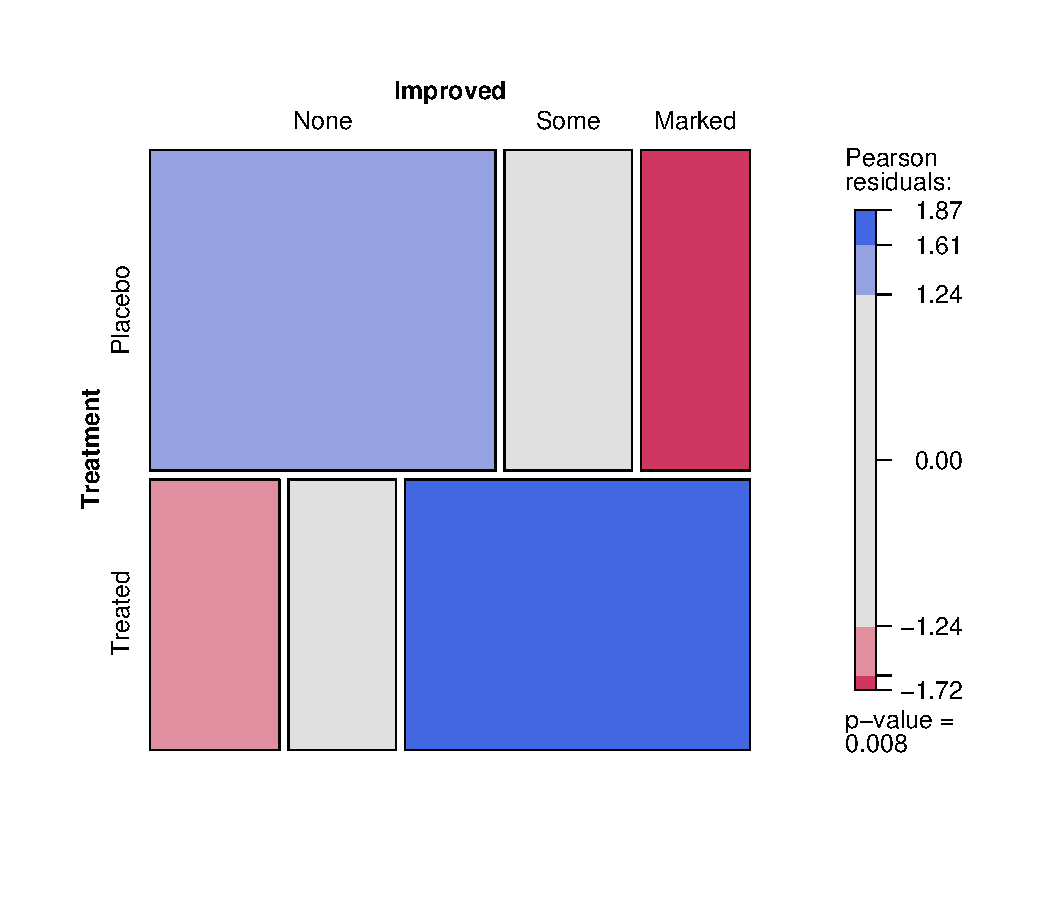
\includegraphics{strucplot-arthritisfig}
\caption{The \data{Arthritis} data (female patients) with significant maximum test.}
\label{fig:maximum}
\end{center}
\end{figure}

\noindent The maximum test is significant although the residuals are
all in the $\left[-2,2\right]$ interval.
The \codefun{shading\_hcl} function with default cut-off points would
not have shown any color. In addition, since the test statistic is the
maximum of the absolute Pearson residuals, \emph{each} colored
residual violates the null hypotheses of independence, and thus, the
``culprits'' can immediately be identified.

\clearpage
\section[Labeling]{Labeling}
\label{sec:labeling}

One of the major enhancements in package \pkg{vcd} compared to
\codefun{mosaicplot} and \codefun{assocplot} in
base \proglang{R} is the labeling in the strucplot framework which 
offers more features and greater flexibility. 
Like shading, spacing, and drawing of legend and core plot, 
labeling is now carried out by grapcon functions, rendering labeling completely
modular.
The user supplies either a labeling function, or, alternatively, 
a generating function that parameterizes a labeling function, 
to \codefun{strucplot} which then draws the labels.
Labeling is well-separated from the actual plotting that occurs in the
low-level core functions. It only relies on the viewport tree produced by them, and the
\code{dimnames} attribute of the visualized table. Labeling
functions are grapcons that ``add ink to the canvas'': the drawing of the
labels happens after the actual plot has been drawn by the core function.
Thus, it is possible to supply one's own labeling function, or
to combine some of the basic functions to produce a more complex labeling.
In the following, we describe the three basic modules
(\codefun{labeling\_text}, \codefun{labeling\_list}, and \codefun{labeling\_cells}) and
derived functions that build upon them.

\subsection[Labels in the borders]{Labels in the borders: \texttt{labeling\_text()}}

\codefun{labeling\_text} is the default for all strucplot displays. It
plots labels in the borders similar to the \codefun{mosaicplot}
function in base \proglang{R}, but is much more flexible: it is not limited
to 4 dimensions, and the positioning and graphical parameters 
of levels and variable names are customizable. In addition,
the problem of overlapping labels can be handled in several ways. 

As an example, again consider the \data{Titanic} data:
by default, the variable names and levels are plotted ``around'' the
plot in a counter-clockwise way (see Figure~\ref{fig:labels1}, top left):

\begin{Schunk}
\begin{Sinput}
> mosaic(Titanic)
\end{Sinput}
\end{Schunk}

% \begin{figure}[p]
% \begin{center}
% <<defaultfig,fig=TRUE,echo=FALSE>>=
% <<default>>
% @
% \caption{Mosaic plot for the \data{Titanic} data with default settings
%   for labeling.}
% \label{fig:defaults}
% \end{center}
% \end{figure}

\noindent Note that the last two levels of the \code{survived} variable do
overlap, as well as some adult and child labels of the \code{age} Variable.
This issue can be addressed in several ways. The ``brute force''
method is to enable clipping for these dimensions (see
Figure~\ref{fig:labels1}, top right):

\begin{Schunk}
\begin{Sinput}
> mosaic(Titanic, labeling_args = list(clip = c(Survived = TRUE, 
+     Age = TRUE)))
\end{Sinput}
\end{Schunk}

% \begin{figure}[p]
% \begin{center}
% <<clippingfig,fig=TRUE,echo=FALSE>>=
% <<clipping>>
% @
% \caption{The effect of clipping.}
%  \label{fig:clipping}
% \end{center}
% \end{figure}

\noindent The \code{clip} parameter is passed to the labeling function
via the \code{labeling\_args} argument which takes a list of
parameters. \code{clip} itself takes a vector of logicals (one for
each dimension). 
% as mentioned before
Almost all vectorized arguments in the strucplot
framework can be abbreviated in the following way: unnamed components
(or the defaults, if there are none) are recycled as needed, but
overridden by the named components. Here, the default is \code{FALSE},
and therefore clipping is enabled only for the \code{survived} and \code{age} variables.
A more sensible solution to the overlap problem is to abbreviate the 
levels (see Figure~\ref{fig:labels1}, middle left):

\begin{Schunk}
\begin{Sinput}
> mosaic(Titanic, labeling_args = list(abbreviate = c(Survived = TRUE, 
+     Age = 3)))
\end{Sinput}
\end{Schunk}

% \begin{figure}[h]
% \begin{center}
% <<abbreviatingfig,fig=TRUE,echo=FALSE>>=
% <<abbreviating>>
% @
% \caption{Abbreviating.}
% \label{fig:abbreviating}
% \end{center}
% \end{figure}

\noindent The \code{abbreviate} argument takes a vector of
integers indicating the number of significant characters the levels should be
abbreviated to (\code{TRUE} is interpreted as 1, obviously). Abbreviation
is performed using the \codefun{abbreviate} function in base \proglang{R}. Another
possibility is to rotate the levels (see Figure~\ref{fig:labels1}, bottom):

\begin{Schunk}
\begin{Sinput}
> mosaic(Titanic, labeling_args = list(rot_labels = c(bottom = 90, 
+     right = 0), offset_varnames = c(right = 1), offset_labels = c(right = 0.3)), 
+     margins = c(right = 4, bottom = 3))
\end{Sinput}
\end{Schunk}

% \begin{figure}[p]
% \begin{center}
% <<rotatefig,fig=TRUE,echo=FALSE,height=6>>=
% <<rotate>>
% @
% \caption{Rotating labels.}
% \label{fig:rotating}
% \end{center}
% \end{figure}

\noindent Finally, we could also inhibit the output of repeated levels 
(see Figure~\ref{fig:labels1}, middle right):

\begin{Schunk}
\begin{Sinput}
> mosaic(Titanic, labeling_args = list(rep = c(Survived = FALSE, 
+     Age = FALSE)))
\end{Sinput}
\end{Schunk}

\setkeys{Gin}{width=0.9\textwidth}
\begin{figure}[p]
\begin{center}
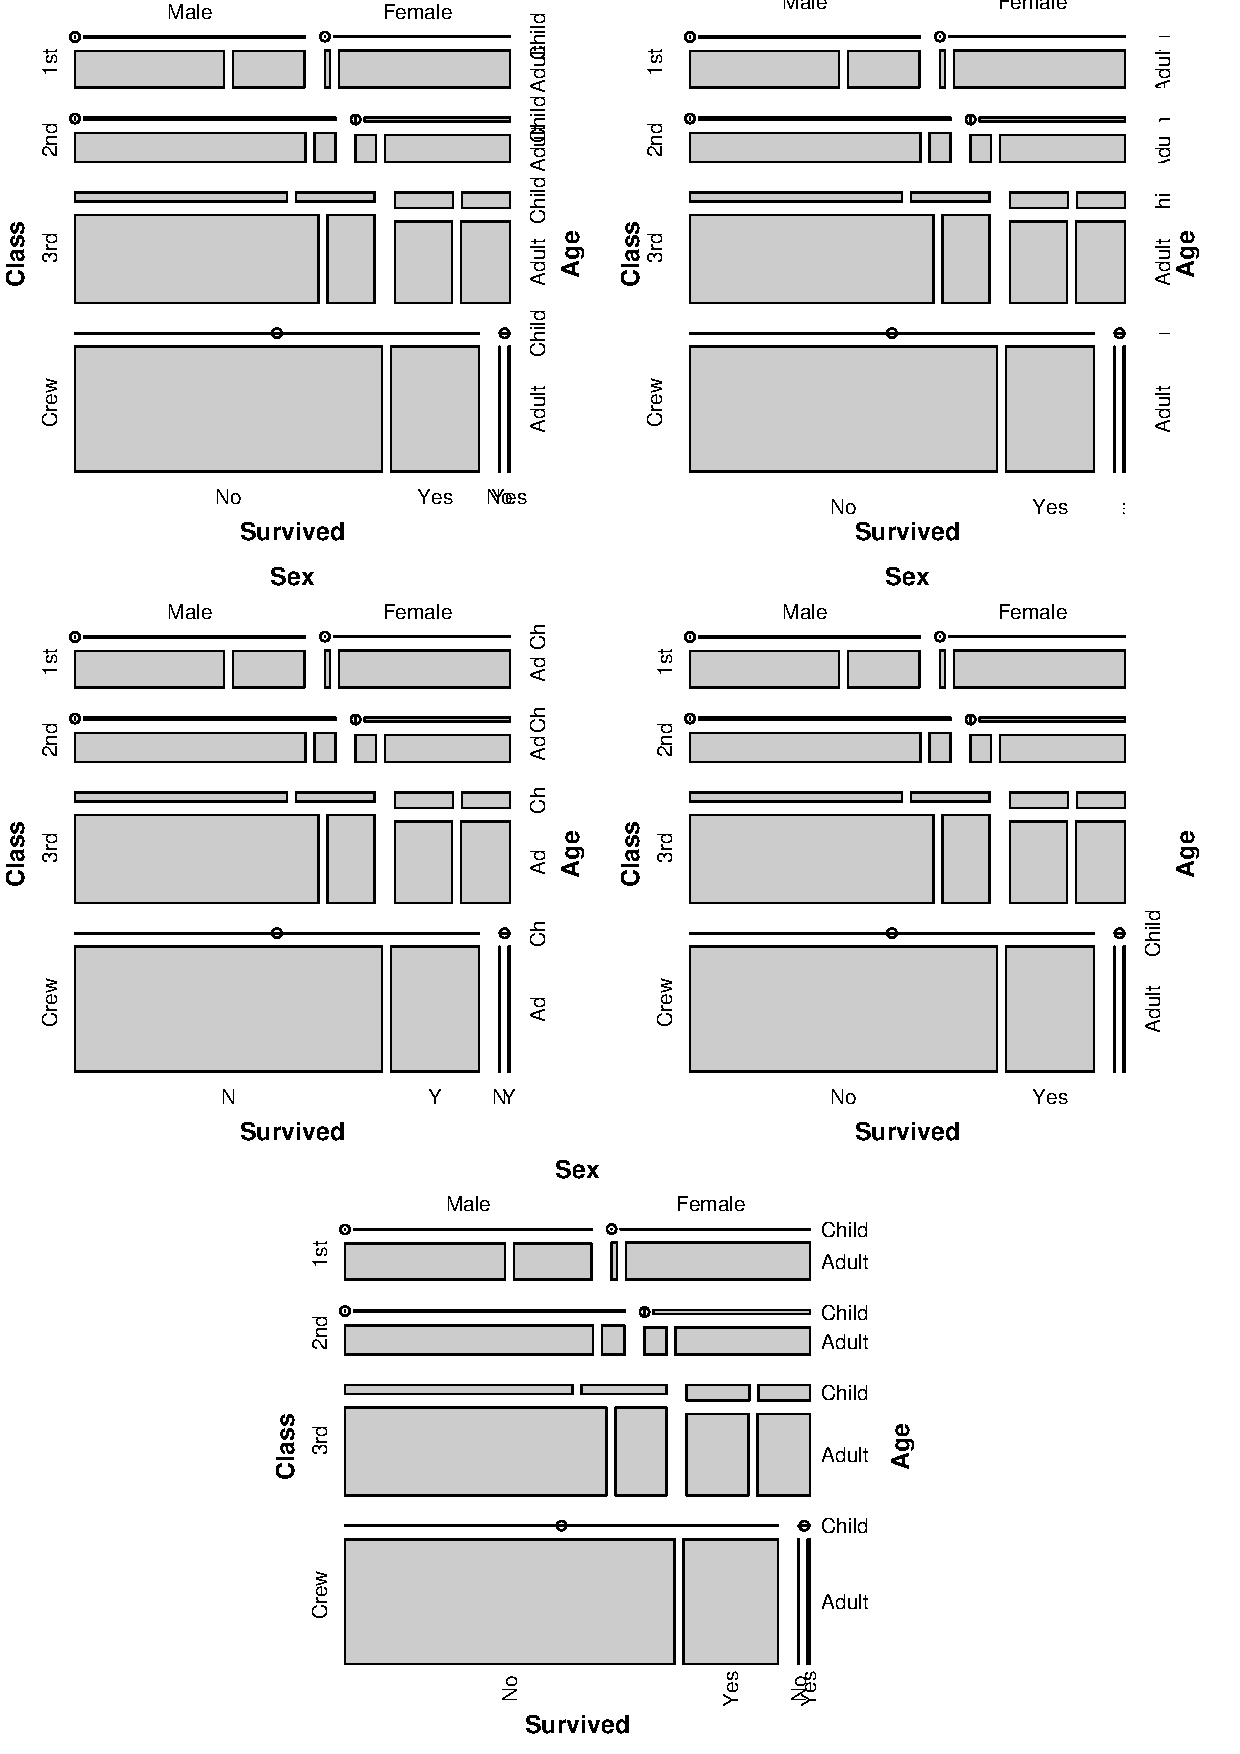
\includegraphics{strucplot-label1fig}
\caption{Examples for possible labeling strategies for the Titanic data mosaic. 
  Top left: default labeling (many labels overlap). 
  Top right: with clipping turned on. Middle left: \texttt{Age} and
  \texttt{Survived} labels abbreviated. Middle right: \texttt{Age} labels
  not repeated. Bottom: \texttt{Age} and \texttt{Survived} labels rotated.}
\label{fig:labels1}
\end{center}
\end{figure}
\setkeys{Gin}{width=0.7\textwidth}

We now proceed with a few more ``cosmetic'' features (which do not all
produce satisfactory results for our sample data).
A first simple, but effectful modification is to position
all labels and variables left-aligned (see Figure~\ref{fig:labels2},
top left):

\begin{Schunk}
\begin{Sinput}
> mosaic(Titanic, labeling_args = list(pos_varnames = "left", 
+     pos_labels = "left", just_labels = "left", rep = FALSE))
\end{Sinput}
\end{Schunk}

% \begin{figure}[h]
% \begin{center}
% <<leftfig,fig=TRUE,echo=FALSE>>=
% <<left>>
% @
% \caption{Left-aligning.}
% \label{fig:left}
% \end{center}
% \end{figure}

\noindent Note that obviously we need to change the justification 
to \code{"left"} as well. We can
achieve the same effect by using the convenience function \codefun{labeling\_left}: 

\begin{Schunk}
\begin{Sinput}
> mosaic(Titanic, labeling = labeling_left)
\end{Sinput}
\end{Schunk}

\noindent Next, we show how to put all levels to the
bottom and right margins, and all variable names to the top and left
margins (see Figure~\ref{fig:labels2}, top right):

\begin{Schunk}
\begin{Sinput}
> mosaic(Titanic, labeling_args = list(tl_labels = FALSE, 
+     tl_varnames = TRUE, abbreviate = c(Survived = 1, 
+         Age = 3)))
\end{Sinput}
\end{Schunk}

% \begin{figure}[p]
% \begin{center}
% <<marginsfig,fig=TRUE,echo=FALSE,height=6>>=
% <<margins>>
% @
% \caption{Changes in the margins.}
% \label{fig:margins}
% \end{center}
% \end{figure}

\noindent The tl\_\var{foo} (``top left'') arguments are \code{TRUE} by default. 
Now, we will add boxes to the labels and additionally
enable clipping (see Figure~\ref{fig:labels2}, bottom left):

\begin{Schunk}
\begin{Sinput}
> mosaic(Titanic, labeling_args = list(tl_labels = FALSE, 
+     tl_varnames = TRUE, boxes = TRUE, clip = TRUE))
\end{Sinput}
\end{Schunk}

% \begin{figure}[p]
% \begin{center}
% <<boxesfig,fig=TRUE,echo=FALSE,height=6>>=
% <<boxes>>
% @
% \caption{Boxes and Clipping.}
% \label{fig:boxes}
% \end{center}
% \end{figure}

\noindent The values to \code{boxes} and \code{clip} are recycled for
all dimensions. The result is pretty close to what calling
\codefun{mosaic} with the \codefun{labeling\_cboxed}
wrapper does, except that variables and levels, by default, are put to the top and
to the left of the plot:

\begin{Schunk}
\begin{Sinput}
> mosaic(Titanic, labeling = labeling_cboxed)
\end{Sinput}
\end{Schunk}

\noindent Another variant is to put the variable names into the
same line as the levels (see Figure~\ref{fig:labels2}, bottom
right---clipping for \code{Survived} and \code{Age} is, additionally,
disabled, and \code{Age} abbreviated):

\begin{Schunk}
\begin{Sinput}
> mosaic(Titanic, labeling_args = list(tl_labels = TRUE, 
+     boxes = TRUE, clip = c(Survived = FALSE, Age = FALSE, 
+         TRUE), abbreviate = c(Age = 4), labbl_varnames = TRUE), 
+     margins = c(left = 4, right = 1, 3))
\end{Sinput}
\end{Schunk}

% \begin{figure}[h]
% \begin{center}
% <<labblfig,fig=TRUE,echo=FALSE>>=
% <<labbl>>
% @
% \caption{Variable names beneath levels, and clipping disabled for the
%   survival variable.}
% \label{fig:labbl}
% \end{center}
% \end{figure}

\noindent \code{labbl\_varnames} (``variable names to the bottom/left of the
labels'') is a vector of logicals indicating the side for the
variable names. The resulting layout is close to what
\codefun{labeling\_lboxed} produces, except that variables and levels,
by default, are left-aligned and put to the bottom and to the right of the plot:

\begin{Schunk}
\begin{Sinput}
> mosaic(Titanic, labeling = labeling_lboxed, margins = c(right = 4, 
+     left = 1, 3))
\end{Sinput}
\end{Schunk}

\noindent A similar design is used by the \codefun{doubledecker} function.

\setkeys{Gin}{width=\textwidth}
\begin{figure}[p]
\begin{center}
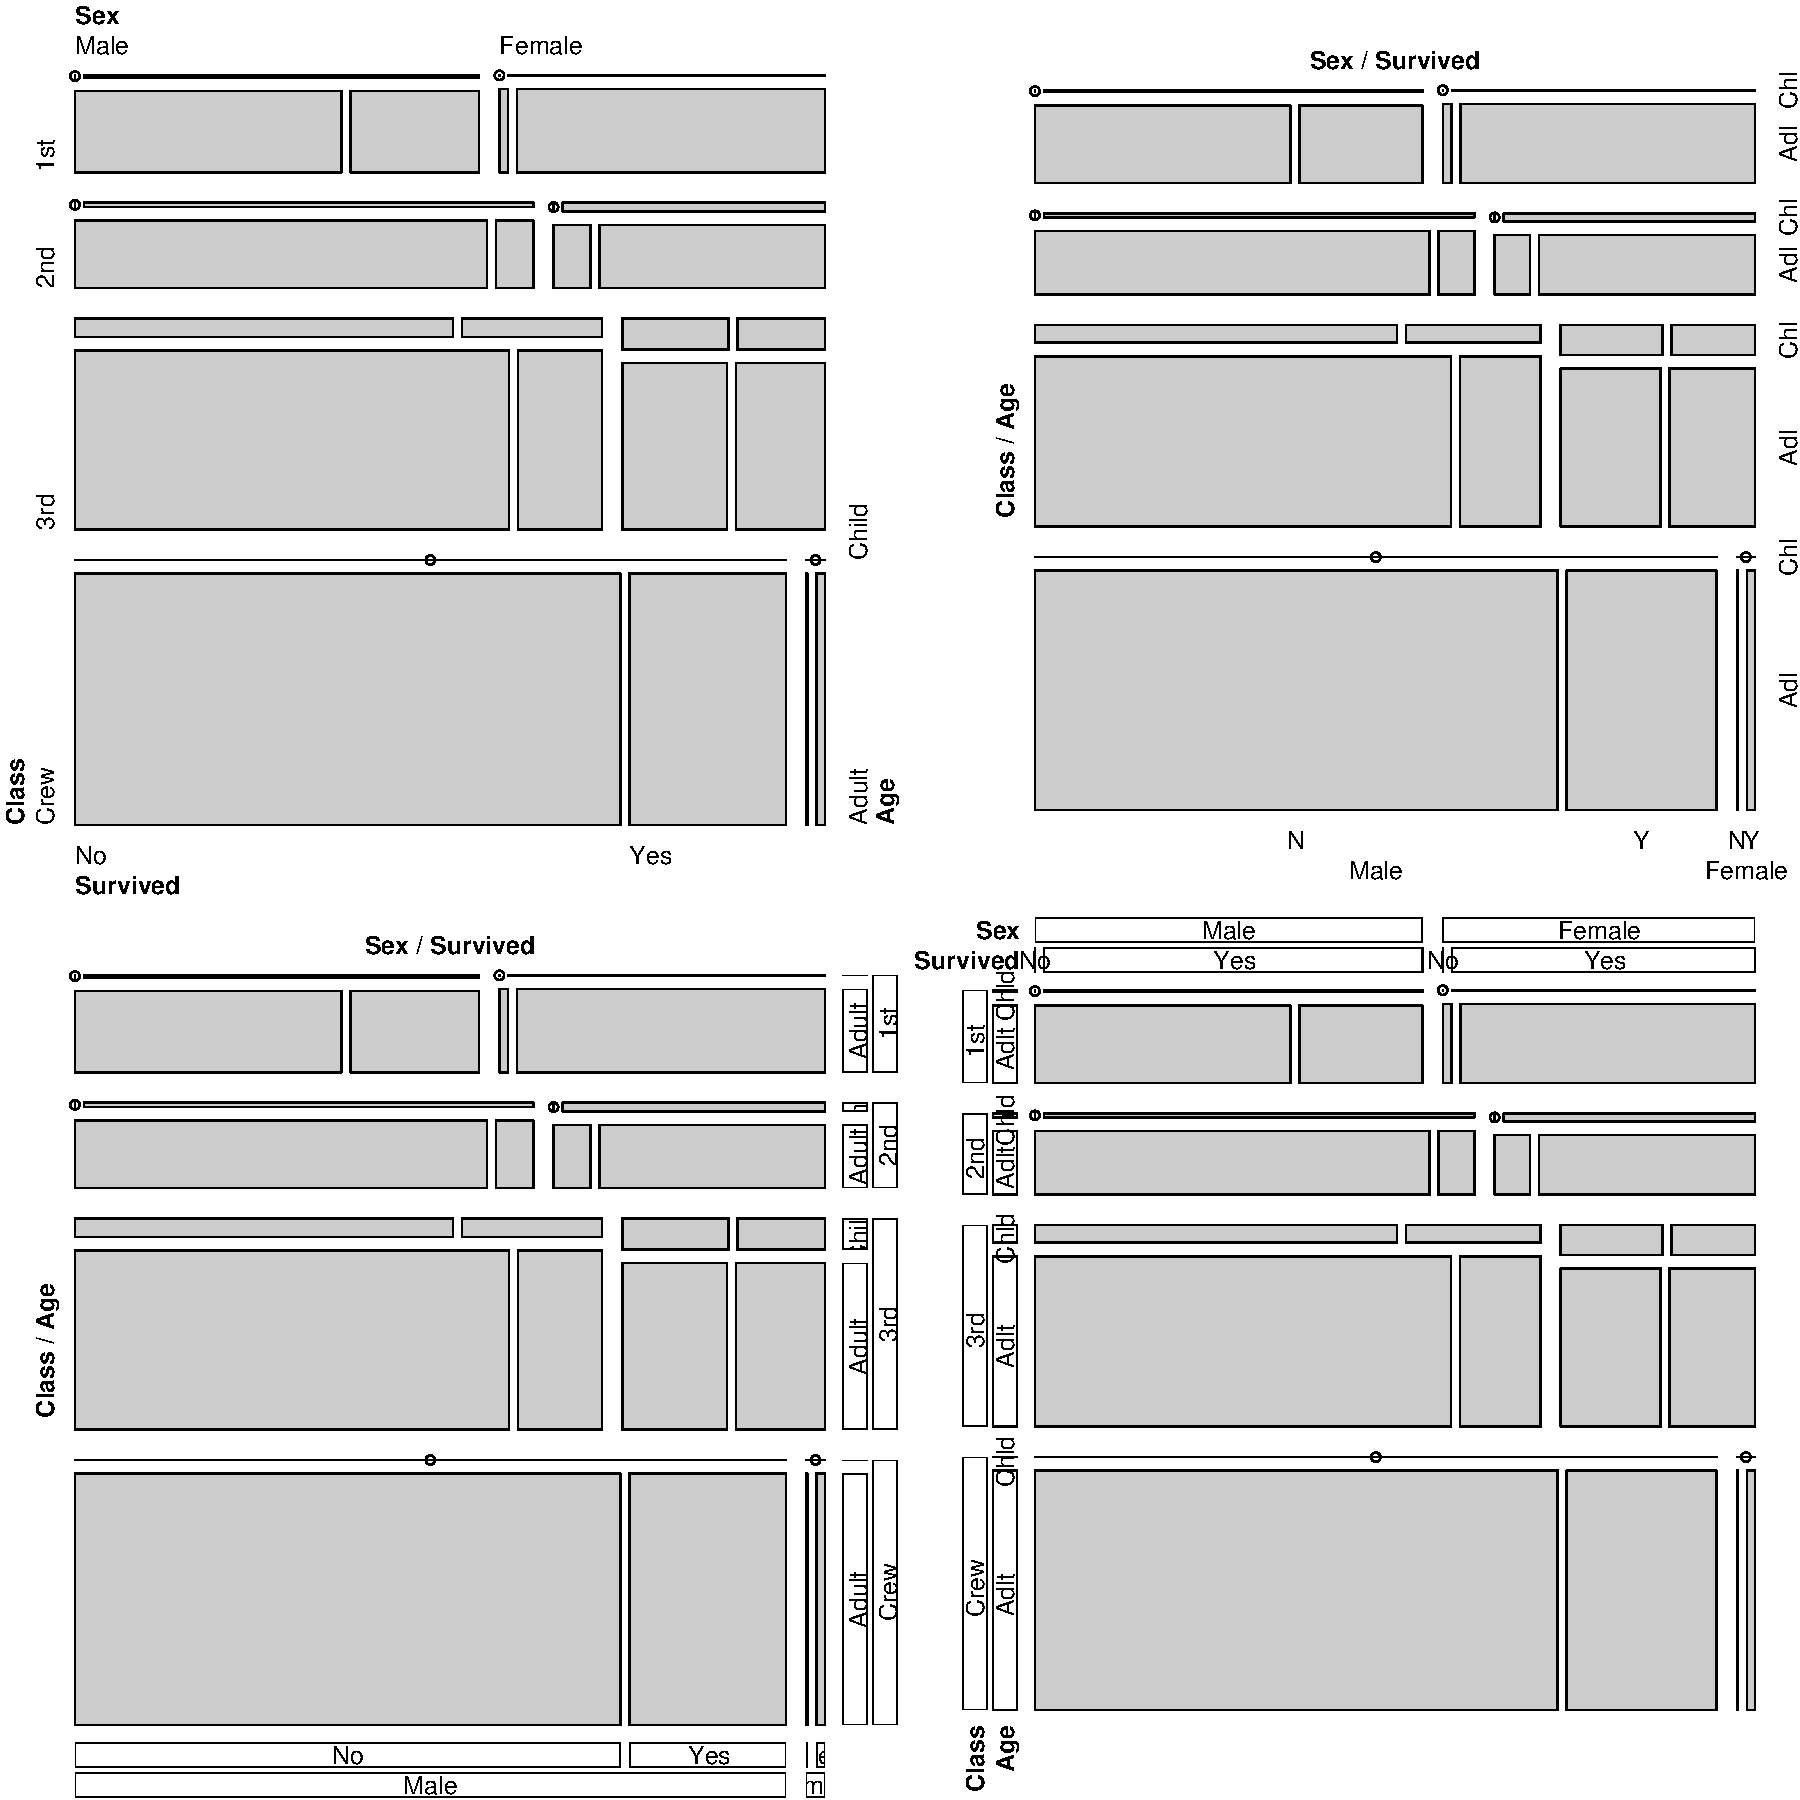
\includegraphics{strucplot-label2fig}
\caption{Advanced strategies for labeling of the Titanic data. Top
  left: left aligning of both variable names and labels. 
  Top right: changes in the margins (all variable names are in the top
  and left margins, and all labels in the bottom and right margins). 
  Bottom left: clipping turned on, and boxes used. Bottom right: 
  variable names beneath levels, clipping disabled for the
  survival and age variables, and \texttt{Age} abbreviated.}
\label{fig:labels2}
\end{center}
\end{figure}
\setkeys{Gin}{width=0.7\textwidth}

\subsection[Labels in the cells]{Labels in the cells: \texttt{labeling\_cells()}}

This labeling draws both variable names and levels in the
cells. As an example, we use the \data{PreSex} data on pre- and
extramarital sex and divorce (see Figure~\ref{fig:labels3}, top left):

\begin{Schunk}
\begin{Sinput}
> mosaic(~MaritalStatus + Gender, data = PreSex, labeling = labeling_cells)
\end{Sinput}
\end{Schunk}

% \begin{figure}[h]
% \begin{center}
% <<cellfig,fig=TRUE,echo=FALSE,width=7,height=7>>=
% <<cell>>
% @
% \caption{Cell labeling for the \data{PreSex} data.}
% \label{fig:cell}
% \end{center}
% \end{figure}

\noindent In the case of narrow cells, it might be useful to
abbreviate labels and/or variable names and turn off clipping (see
Figure~\ref{fig:labels3}, top right):

\begin{Schunk}
\begin{Sinput}
> mosaic(~PremaritalSex + ExtramaritalSex, data = PreSex, 
+     labeling = labeling_cells(abbreviate_labels = TRUE, 
+         abbreviate_varnames = TRUE, clip = FALSE))
\end{Sinput}
\end{Schunk}

% \begin{figure}[h]
% \begin{center}
% <<cell2fig,fig=TRUE,echo=FALSE>>=
% <<cell2>>
% @
% \caption{Cell labeling for the \data{PreSex} data, labels abbreviated.}
% \label{fig:cell2}
% \end{center}
% \end{figure}

\noindent For some data, it might be convenient to combine cell
labeling with border labeling as done by \codefun{labels\_conditional}
(see Figure~\ref{fig:labels3}, bottom left):

\begin{Schunk}
\begin{Sinput}
> mosaic(~PremaritalSex + ExtramaritalSex | MaritalStatus + 
+     Gender, data = PreSex, labeling = labeling_conditional(abbreviate_varnames = TRUE, 
+     abbreviate_labels = TRUE, clip = FALSE, gp_text = gpar(col = "red")))
\end{Sinput}
\end{Schunk}

% \begin{figure}[h]
% \begin{center}
% <<conditionalfig,fig=TRUE,echo=FALSE>>=
% <<conditional>>
% @
% \caption{Conditional labeling for the \data{PreSex} data, labels (in
%   red for clarity) abbreviated.}
% \label{fig:conditional}
% \end{center}
% \end{figure}

\noindent Additionally, the cell labeling allows the user to add
arbitrary text to the cells by supplying a character array in the same
shape as the data array to the \code{text} argument (cells with missing values
are ignored). In the following example using the \code{Titanic} data, 
this is used to add all observed values greater
than 5 to the cells after the mosaic has been plotted (see
Figure~\ref{fig:labels3}, bottom right):

\begin{Schunk}
\begin{Sinput}
> mosaic(Titanic, labeling_args = list(abbreviate = c(Survived = 1, 
+     Age = 4)), pop = FALSE)
> tab <- ifelse(Titanic < 6, NA, Titanic)
> labeling_cells(text = tab, clip = FALSE)(Titanic)
\end{Sinput}
\end{Schunk}

% \begin{figure}[h]
% \begin{center}
% <<textfig,fig=TRUE,echo=FALSE>>=
% <<text>>
% @
% \caption{User-supplied text (observed frequencies exceeding 5) 
% added to a mosaic display of the \data{Titanic} data.}
% \label{fig:text}
% \end{center}
% \end{figure}


\setkeys{Gin}{width=\textwidth}
\begin{figure}[p]
\begin{center}
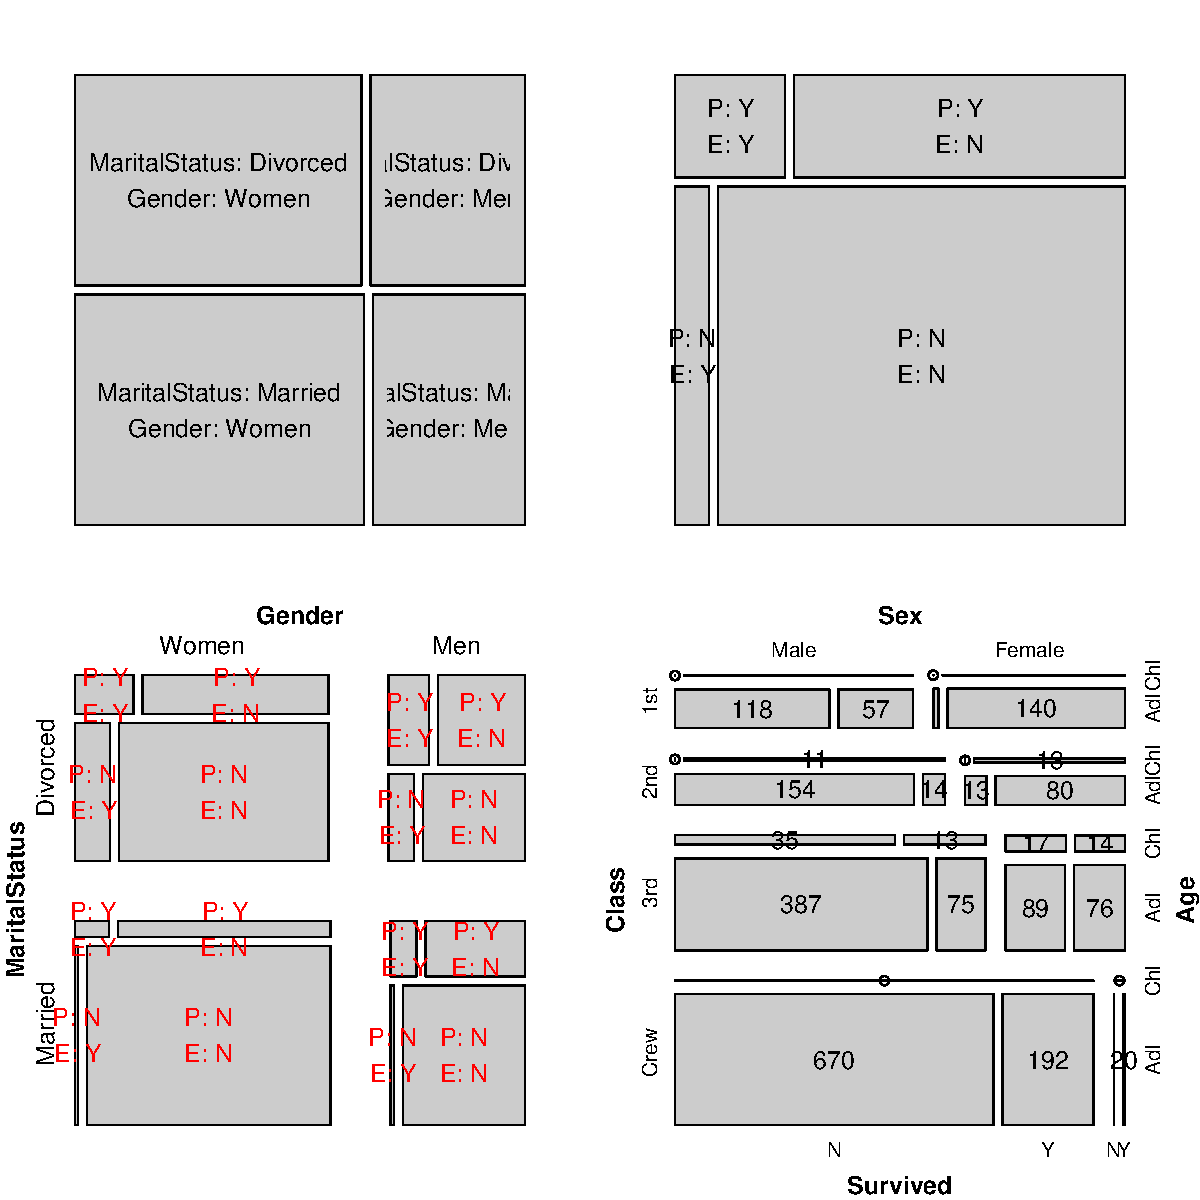
\includegraphics{strucplot-label3fig}
\caption{Cell labeling. Top left: default labeling using the
  \data{PreSex} data. Top right: abbreviated labels. Bottom left:
  conditional labeling (labels abbreviated and in red for clarity).
  Bottom right: user-supplied text (observed frequencies exceeding 5) 
  added to a mosaic display of the \data{Titanic} data. Note that
  clipping is on by default (top left), and has explicitly been turned
  off for the three other plots.}
\label{fig:labels3}
\end{center}
\end{figure}
\setkeys{Gin}{width=0.7\textwidth}

\subsection[A simple list of labels]{A simple list of labels: \texttt{labeling\_list()}}

If problems with overlapping labels cannot satisfactorily resolved,
the last remedy could be to simply list the levels below the plot
(see Figure~\ref{fig:list}):

\begin{Schunk}
\begin{Sinput}
> mosaic(Titanic, labeling = labeling_list, margins = c(bottom = 5))
\end{Sinput}
\end{Schunk}

\setkeys{Gin}{width=0.7\textwidth}
\begin{figure}[p]
\begin{center}
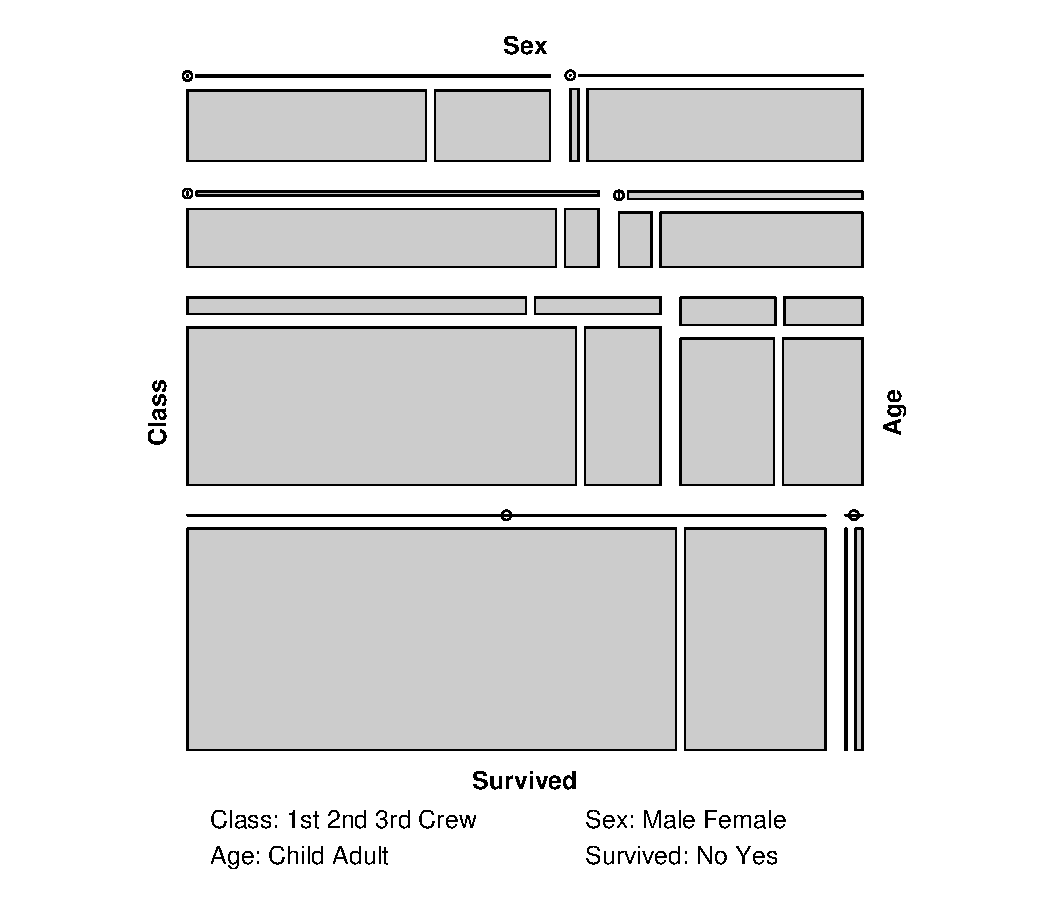
\includegraphics{strucplot-listfig}
\caption{Labels indicated below the plot.}
\label{fig:list}
\end{center}
\end{figure}

\noindent The number of columns can be specified.

\section{Spacing}
\label{sec:spacing}

Spacing of strucplot displays is customizable in a similar way than shading. The
\code{spacing} argument of the \codefun{strucplot} function takes a
list of \class{unit} vectors, one for each dimension, specifying the
space between the tiles corresponding to the levels. 
Consider again the introductory example of the \data{Arthritis} data 
(Figure~\ref{fig:arthritis}). Since we are interested in the effect of
the medicament in the placebo and treatment groups, a mosaic plot is
certainly appropriate to visualize the three levels of \code{Improved} in
the two \code{Treatment} strata. Another conceptual approach is to use
spine plots with highlighting \citep{vcd:hummel:1996}. A spine plot is
a variation of a bar plot where the heights of the bars are held
constant, whereas the widths are used to represent the number of cases
in each category. This is equivalent to a mosaic plot for a one-way table.
If a second (indicator) variable is highlighted in a spine plot, we
obtain a display equivalent to a simple mosaic display for a two-way
table, except that no space between the levels of the highlighted
variable is used.
In the \data{Arthritis} example, we will highlight patients with \code{Marked} 
improvement in both groups. To obtain such a display within 
the strucplot framework, it suffices to set the space between the \code{Improved}
tiles to 0 (see Figure~\ref{fig:artspine}):

\begin{Schunk}
\begin{Sinput}
> (art <- structable(~Treatment + Improved, data = Arthritis, 
+     split_vertical = TRUE))
\end{Sinput}
\begin{Soutput}
         Treatment Placebo Treated
Improved                          
None                    29      13
Some                     7       7
Marked                   7      21
\end{Soutput}
\begin{Sinput}
> (my_spacing <- list(unit(0.5, "lines"), unit(c(0, 0), 
+     "lines")))
\end{Sinput}
\begin{Soutput}
[[1]]
[1] 0.5lines

[[2]]
[1] 0lines 0lines
\end{Soutput}
\begin{Sinput}
> my_colors <- c("lightgray", "lightgray", "black")
> mosaic(art, spacing = my_spacing, gp = gpar(fill = my_colors, 
+     col = my_colors))
\end{Sinput}
\end{Schunk}

\begin{figure}[p]
\begin{center}
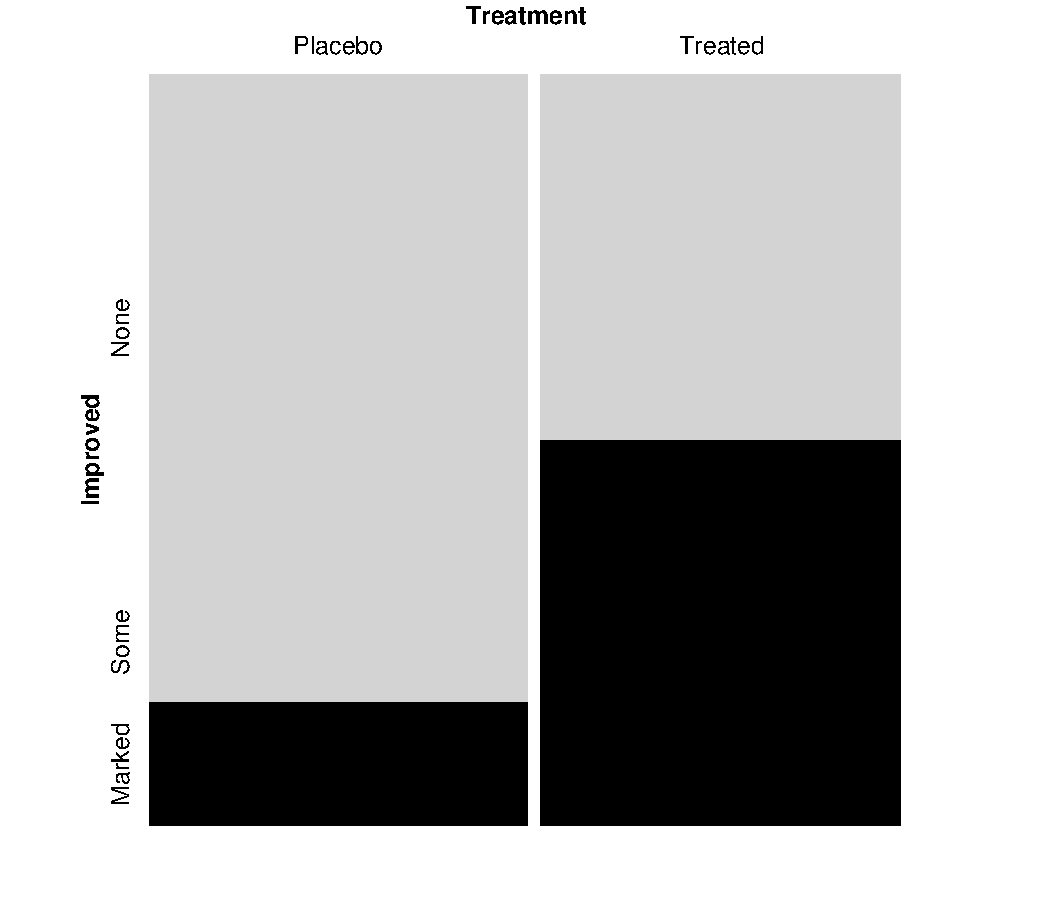
\includegraphics{strucplot-artspinefig}
\caption{Spine plot for the \data{Arthritis} data using the strucplot framework.}
\label{fig:artspine}
\end{center}
\end{figure}

\noindent Note that the default and formula methods for 
\codefun{mosaic} provide a
convenience interface for highlighting. A similar plot (with slightly
different shading) than the previous one can be obtained using:

\begin{Schunk}
\begin{Sinput}
> mosaic(Improved ~ Treatment, data = Arthritis, split_vertical = TRUE)
\end{Sinput}
\end{Schunk}
 
\noindent The strucplot framework also provides a set of spacing grapcon
generators which compute suitable spacing objects for
typical applications. The simplest spacing is \codefun{spacing\_equal}
that uses the same space between all tiles (see
Figure~\ref{fig:spacing}, top left):

\begin{Schunk}
\begin{Sinput}
> mosaic(art, spacing = spacing_equal(unit(2, "lines")))
\end{Sinput}
\end{Schunk}

\noindent \codefun{spacing\_equal} is the default grapcon generator for
two-dimensional tables. Slightly more flexible is \codefun{spacing\_dimequal} that
allows an individual setting for each dimension (see
Figure~\ref{fig:spacing}, top right):

\begin{Schunk}
\begin{Sinput}
> mosaic(art, spacing = spacing_dimequal(unit(1:2, "lines")))
\end{Sinput}
\end{Schunk}

\noindent The default for multi-way contingency tables is
\codefun{spacing\_increase} which uses increasing spaces for the
dimensions. The user can specify a start value and the increase factor
(see Figure~\ref{fig:spacing}, bottom left):

\begin{Schunk}
\begin{Sinput}
> mosaic(art, spacing = spacing_increase(start = unit(0.5, 
+     "lines"), rate = 1.5))
\end{Sinput}
\end{Schunk}

\noindent For the arthritis example above, we could as well have used
\codefun{spacing\_highlighting} which is similar to \codefun{spacing\_increase} but
sets the spacing in the last splitting dimension to 0 (see
Figure~\ref{fig:spacing}, bottom right):

\begin{Schunk}
\begin{Sinput}
> mosaic(art, spacing = spacing_highlighting, gp = my_colors)
\end{Sinput}
\end{Schunk}

\noindent Finally, \codefun{spacing\_conditional} can be used for
visualizing conditional independence: it combines
\codefun{spacing\_equal} (for the conditioned dimensions) and 
\codefun{spacing\_increase} (for the conditioning dimensions). As an example, 
consider Figure~\ref{fig:presex}: the spacing clearly allows to better 
distinguish the conditioning variables 
(\code{Gender} and \code{MaritalStatus}) from the conditioned 
variables (\code{PremaritalSex} and \code{ExtramaritalSex}). This
spacing is the default when conditional variables are specified for a
strucplot display (see Section \ref{sec:strucplot}).


\setkeys{Gin}{width=\textwidth}
\begin{figure}[p]
\begin{center}
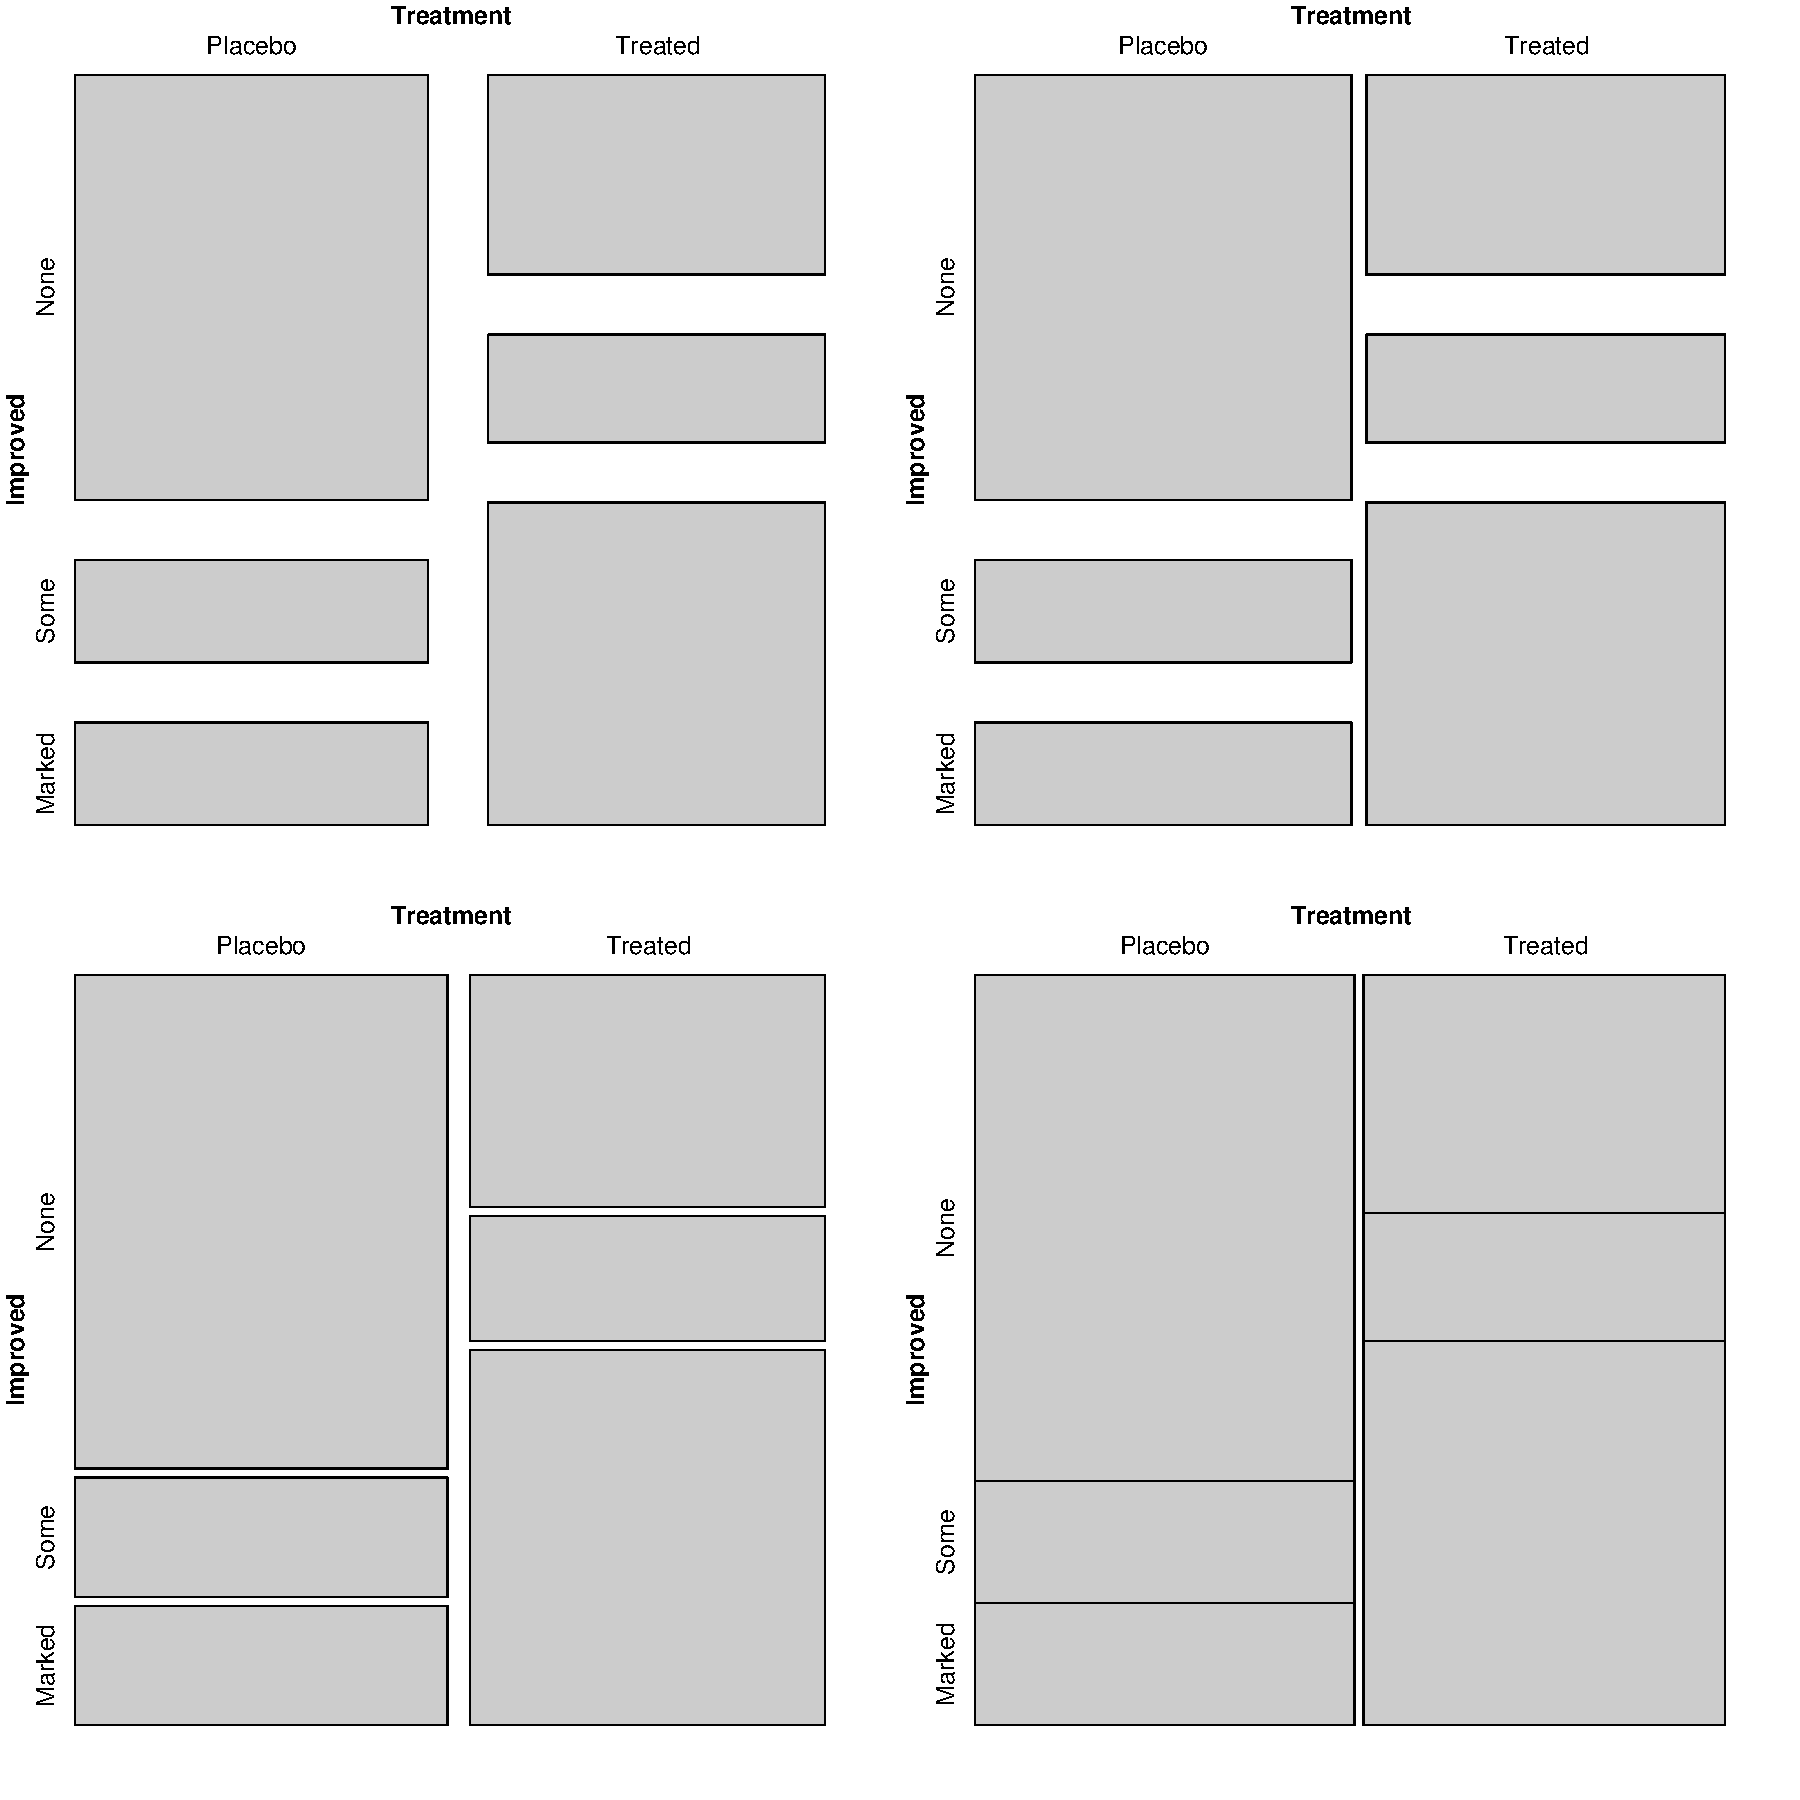
\includegraphics{strucplot-spacingfig}
\caption{Varying spacing for the Arthritis  data. Top left: equal
  spacing for all dimensions. Top right: different spacings for
  individial dimensions. Bottom left: increasing spacing. Bottom right: 
  spacing used for highlighting.}
\label{fig:spacing}
\end{center}
\end{figure}
\setkeys{Gin}{width=0.7\textwidth}


\section{Example: Ovarian cancer survival}
\label{sec:example}

In the following, we demonstrate some of the described techniques in
analyzing a data set originating from \citep{vcd:obel:1975}
\cite[taken from][]{vcd:andersen:1991} about a retrospective study of ovary cancer
carried out in 1973.  Information was obtained from 299 women, who
were operated for ovary cancer 10 years before. The data consists of
four binary variables: the \code{stage} of the cancer at the time of
operation (levels: \code{early}, \code{advanced}), the type of \code{operation} performed
(\code{radical}, \code{limited}), the \code{survival} status after 10 years (\code{yes}, 
\code{no}), and \code{xray} indicating whether X-ray treatment was received (\code{yes},
\code{no}). 

The dataset in \pkg{vcd} comes pretabulated in a data frame, so we
first create the four-way table:

\begin{Schunk}
\begin{Sinput}
> tab <- xtabs(Freq ~ stage + operation + xray + survival, 
+     data = OvaryCancer)
\end{Sinput}
\end{Schunk}

\noindent A ``flattened'' textual representation can be obtained using \codefun{structable}:

\begin{Schunk}
\begin{Sinput}
> structable(survival ~ ., data = tab)
\end{Sinput}
\begin{Soutput}
                        survival no yes
stage    operation xray                
early    radical   no            10  41
                   yes           17  64
         limited   no             1  13
                   yes            3   9
advanced radical   no            38   6
                   yes           64  11
         limited   no             3   1
                   yes           13   5
\end{Soutput}
\end{Schunk}

\noindent A first overview can be obtained using a pairs plot (Figure~\ref{fig:ocpairs}):

\begin{Schunk}
\begin{Sinput}
> dpa <- list(var_offset = 1.2, rot = -30, just_leveltext = "left")
> pairs(tab, diag_panel_args = dpa)
\end{Sinput}
\end{Schunk}

\begin{figure}[h]
\begin{center}
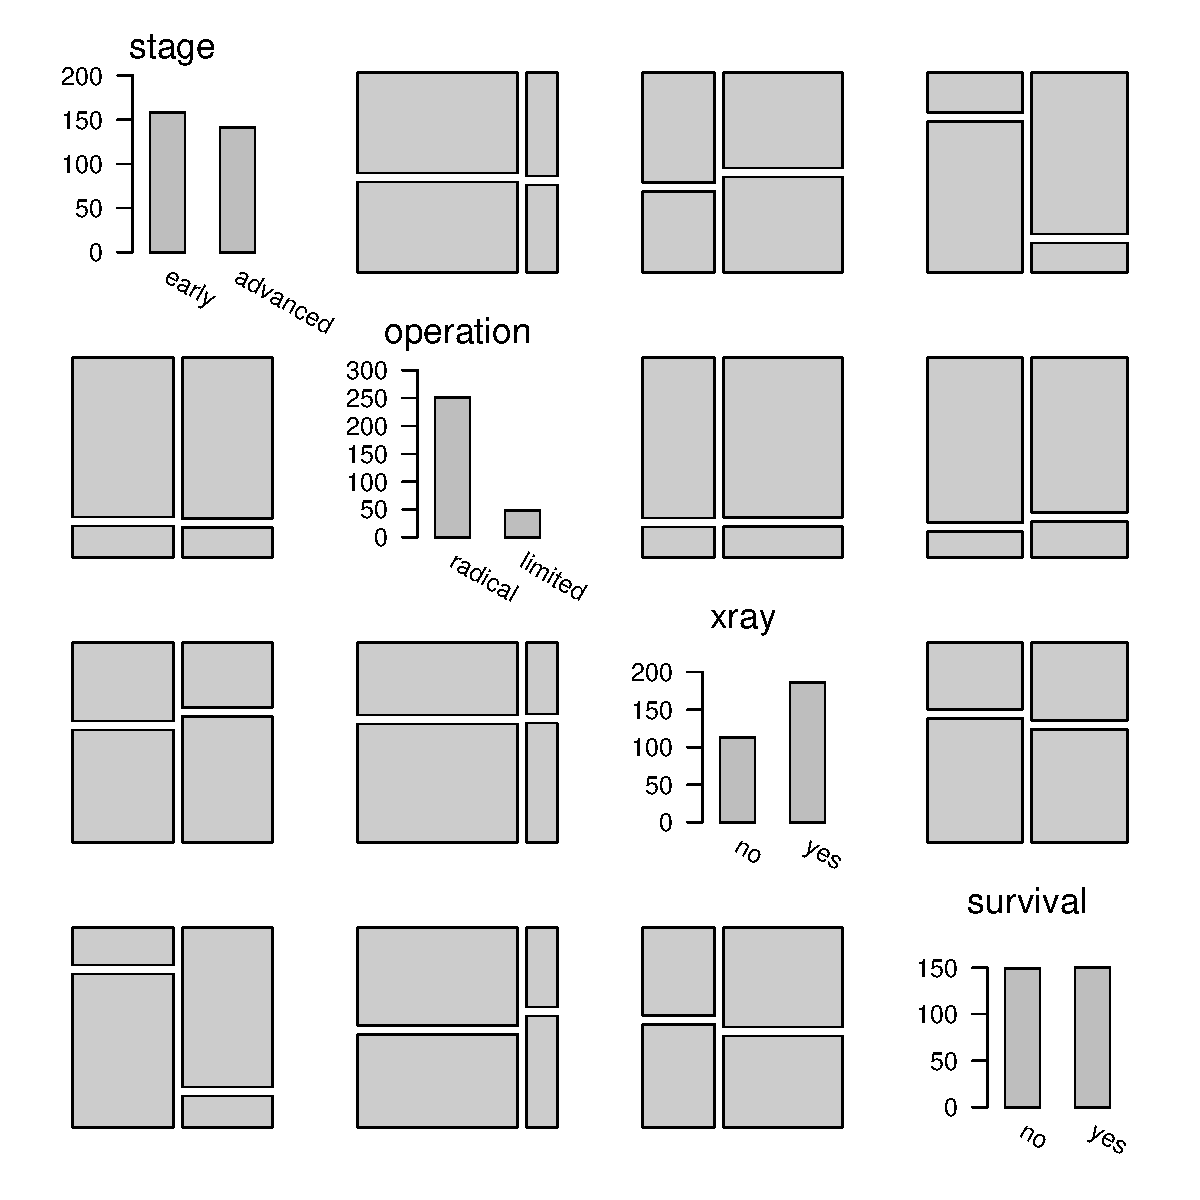
\includegraphics{strucplot-ocpairs}
\caption{Pairs plot for the \data{OvaryCancer} data showing mosaic displays for all pairwise distributions and bar plots for all marginal distributions.}
\label{fig:ocpairs}
\end{center}
\end{figure}

\noindent The pairs plot, by default, creates mosaic displays for all pairwise 
variable combinations, and bar plots in the diagonal to visualize the absolute 
frequencies of the variables. The \texttt{var\_offset} argument modifies the offset of the 
(centered) variable names to avoid overlap with the bars. 
Additionally, we use the \texttt{rot} and the
\texttt{just\_leveltext} arguments to rotate the level names, again to avoid their overlap.
First, we consider the marginal distributions. The study design involved 
(nearly) the same number of survived (150) and deceased (149) patients. Similarly balanced,
158 cases were in an advanced and 141 in an early stage. Most patients (251, 84\%) 
were treated with a radical operation, and 186 (62\%) were submitted to
X-ray treatment. Next, we inspect
the two-way interaction of the influencing factors (\code{stage}, \code{operation}, 
and \code{xray}): the
corresponding mosaics exhibit symmetric, regular shapes with aligned tiles, 
which indicate no marginal interaction between these variables. 
The same is true for the interactions of \code{survival}
with \code{operation} and \code{xray}, respectively. Only the stage seems to influence
survival: here, the tiles are ``shifted''.

A different view on the data, focused on the influence of the
explanatory variables on \code{Survival},
can be obtained using a doubledecker plot (Figure~\ref{fig:ocdoubledecker}):

\begin{Schunk}
\begin{Sinput}
> doubledecker(survival ~ stage + operation + xray, data = tab)
\end{Sinput}
\end{Schunk}

\begin{figure}[h]
\begin{center}
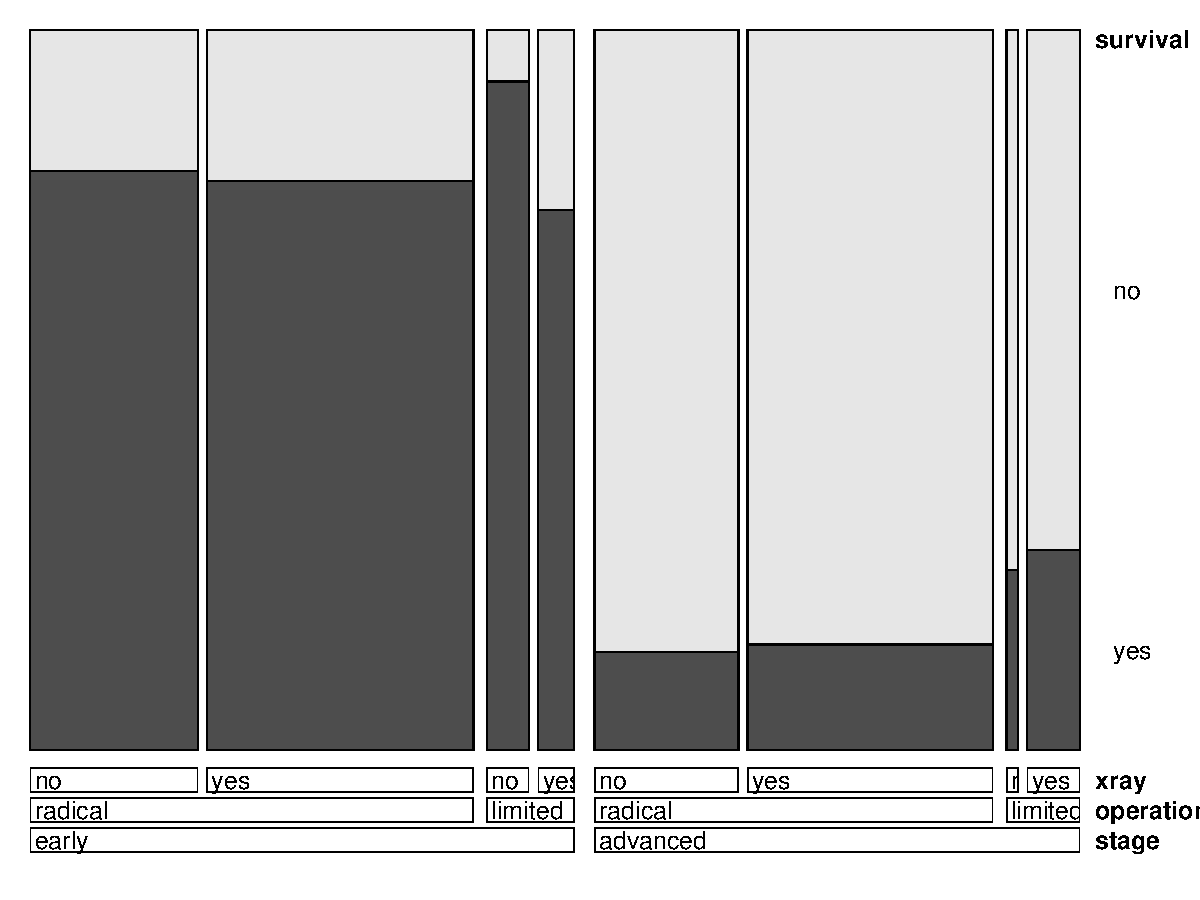
\includegraphics{strucplot-ocdoubledecker}
\caption{Doubledecker plot for the \data{OvaryCancer} data showing the
 conditional distribution of X-ray, given operation, given stage, and with
 survival highlighted.}
\label{fig:ocdoubledecker}
\end{center}
\end{figure}

\noindent From a technical point of view, the display is constructed as a mosaic plot
showing the conditional distribution of \code{survival}, given \code{xray}, 
given \code{operation}, given \code{stage}, 
with vertical splits for the conditioning variables and horizontal ones for
\code{survival}. 
Additionally, there is zero space between the tiles of the last dimension and
a binary shading is used for survived and deceased patients.
Conceptually, this plot is interpreted as a mosaic plot of just the influencing
variables, with \code{survival} highlighted in the tiles. Thus, the plot really shows
the influence of the explanatory variables on \code{survival}. Clearly, the survival
rate is higher among patients in an early stage, but neither radical operation 
nor X-ray treatment seem to improve the situation. From this exploratory
phase, the survival rate seems to be slightly higher for patients who
received a limited operation only, whereas the effect for X-ray
treatment is less marked.

To visualize inference results, we can make use of residual-based
shadings, investigating log-linear models for the four-way table. 
Figure~\ref{fig:ocmosaicnull} visualizes the null model, where
survival is independent from the combined effect of operation, X-ray
treatment, and stage:

\begin{Schunk}
\begin{Sinput}
> split <- c(TRUE, TRUE, TRUE, FALSE)
> mosaic(tab, expected = ~survival + operation * xray * 
+     stage, split_vertical = split)
\end{Sinput}
\end{Schunk}

\begin{figure}[p]
\begin{center}
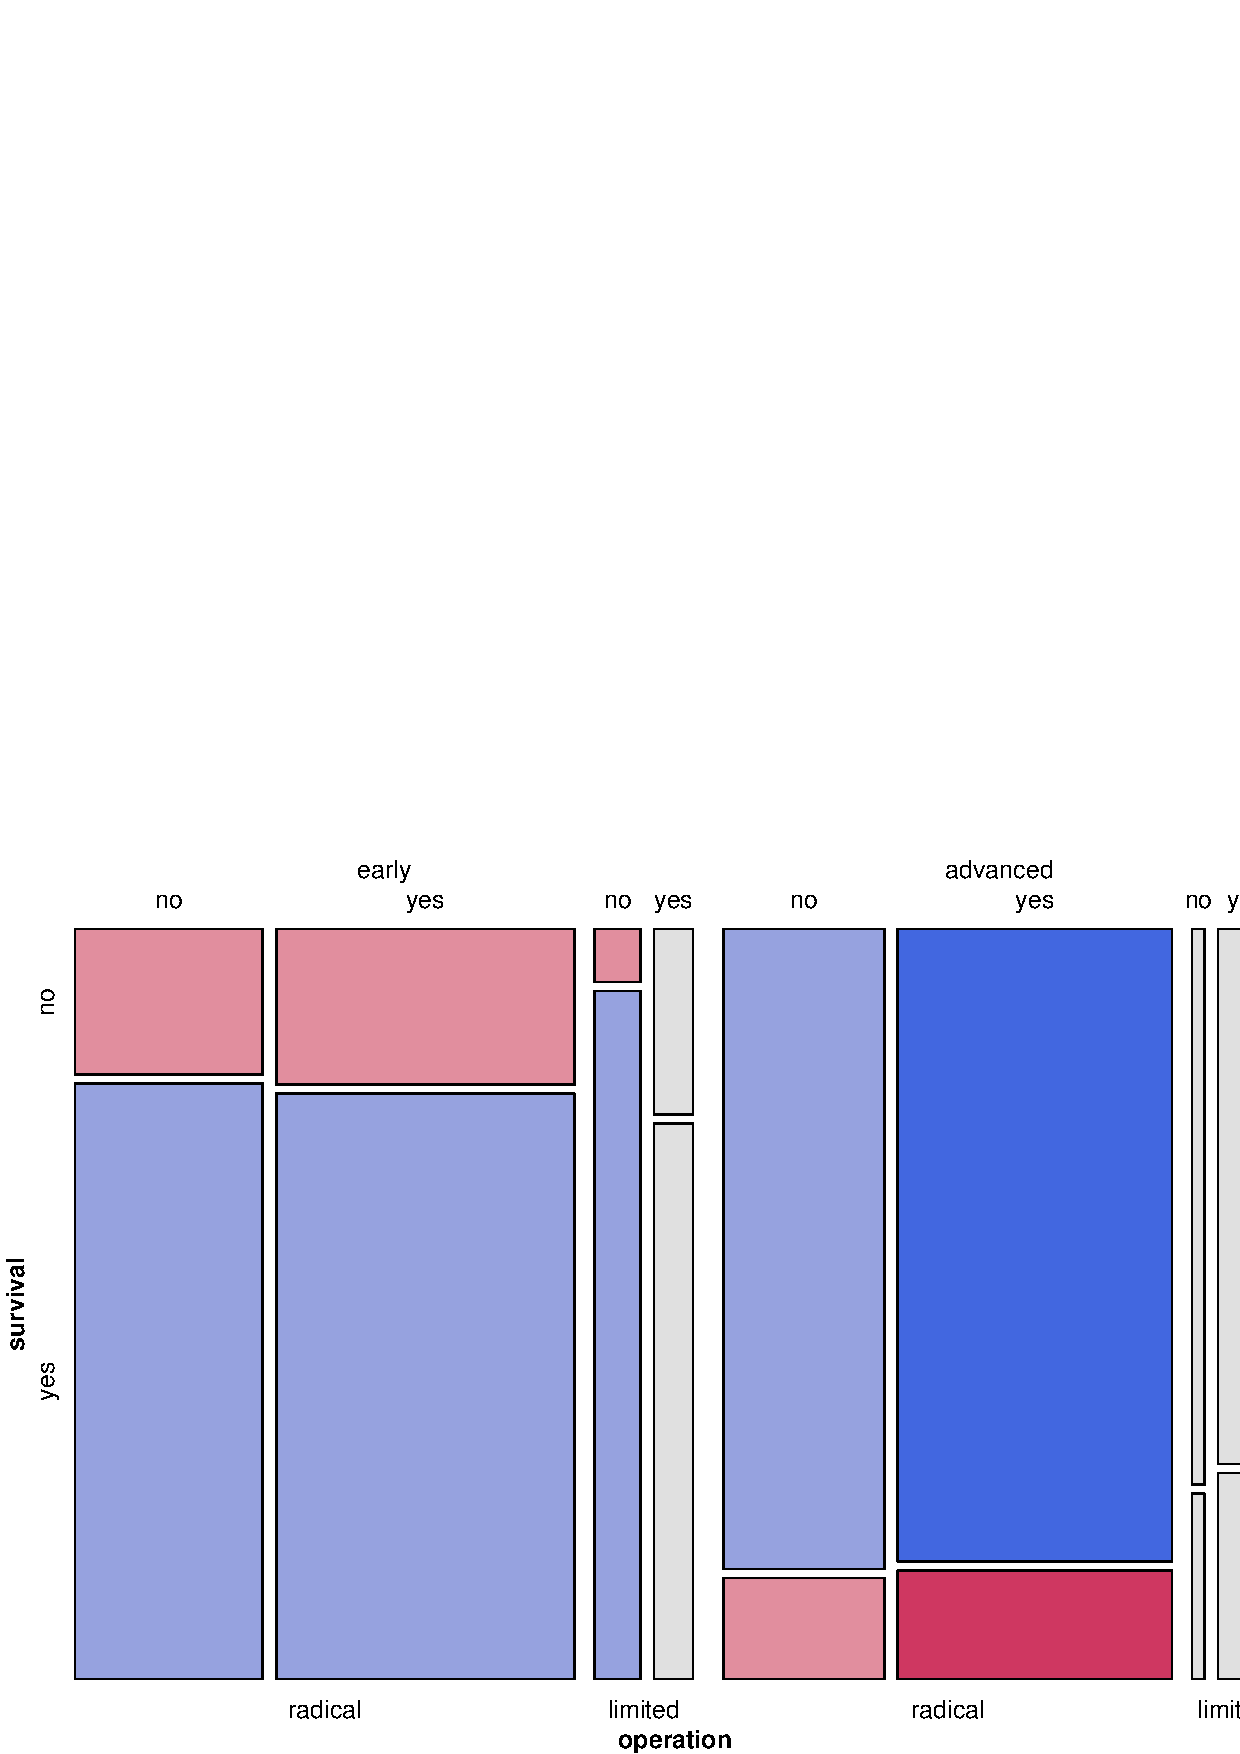
\includegraphics{strucplot-ocmosaicnull}
\caption{Mosaic plot for the \data{OvaryCancer} data, with residual-based shading
for the (clearly rejected) null model (survival)(operation, X-ray, stage).}
\label{fig:ocmosaicnull}
\end{center}
\end{figure}

\noindent The model is clearly rejected ($p$-value: 0.000). From the exploratory phase of
our analysis, we (only) suspect \code{stage} to be influential on the survival rate. A 
corresponding hypothesis is that \code{survival} be independent of \code{xray} 
and \code{operation}, given
\code{stage}. The model is specified using the \texttt{expected} argument, 
either using the \codefun{loglin} interface or 
the \codefun{loglm} formula interface (the resulting mosaic plot is shown in Figure
\ref{fig:ocmosaicstage}):

\begin{Schunk}
\begin{Sinput}
> mosaic(tab, expected = ~(survival + operation * xray) * 
+     stage, split_vertical = split)
\end{Sinput}
\end{Schunk}

\begin{figure}[p]
\begin{center}
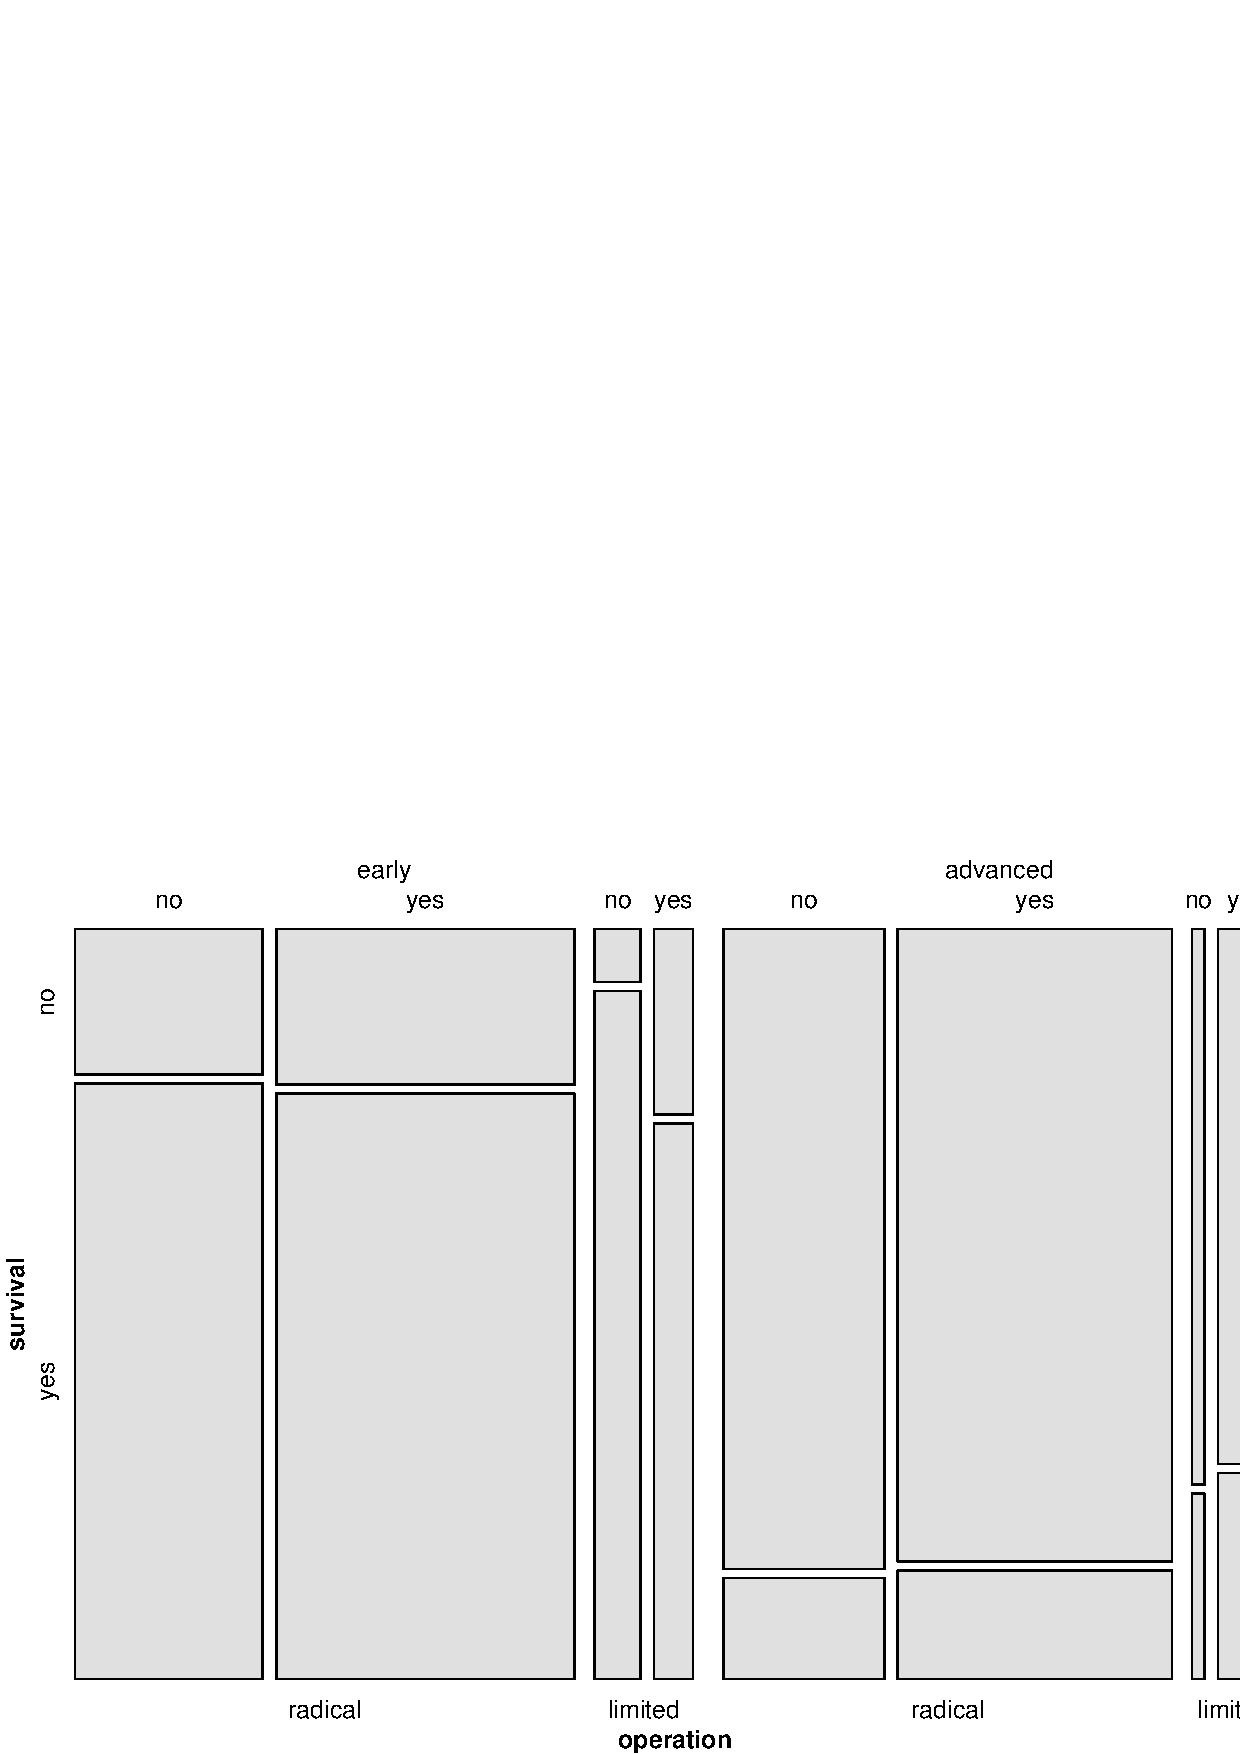
\includegraphics{strucplot-ocmosaicstage}
\caption{Mosaic plot for the \data{OvaryCancer} data, with residual-based shading
for the hypothesis of survival being independent of X-ray and operation, given
stage. The hypothesis is not rejected.}
\label{fig:ocmosaicstage}
\end{center}
\end{figure}

\noindent Thus, based on this data, only pre-diagnosis seems to matter in ovarian
cancer therapy.

\section{Conclusion}
\label{sec:conclusion}

In this paper, we describe the ``strucplot'' framework for the visualization of
multi-way contingency tables. Strucplot displays include popular 
basic plots such as mosaic, association, and sieve plots, integrated 
in a unified framework: all can be seen as visualizations of
hierarchical conditional flat tables. 
Additionally, these core strucplot displays can be combined into more complex, 
specialized plots, such as pairs and trellis-like displays for visualizing
conditional independence. Residual-based shadings permit the
visualization of log-linear models and the results of independence tests.
The framework's modular design allows
flexible customization of the plots' graphical appearance, including 
shading, labeling, spacing, and legend, by means of graphical
appearance control (``grapcon'') functions. These ``graphical
hyperparameters'' are customized and created by
generating functions. Our work includes a set of predefined grapcon generators for
typical analysis tasks, and user-level extensions can easily be added.

\bibliography{vcd}

\begin{appendix}

\section{Data sets}
\label{sex:data}

The data set names in the paper are those from the \proglang{R}
system. In the following, we give a short description of each data set.

\begin{description}
\item[\texttt{Arthritis}] Data  from a 
  double-blind clinical trial
  investigating a new treatment for rheumatoid arthritis. 
  Source: \cite{vcd:Koch+Edwards:1988}. Taken from: \cite{vcd:Friendly:2000}.
  Package: \pkg{vcd}.
\item[\texttt{Bundesliga}] Results from the first German soccer league in the
  years 1995/6 \citep{vcd:Knorr-Held:1999} and 2001/2 (Collected by: Achim
  Zeileis). Package: \pkg{vcd}.
\item[\texttt{HairEyeColor}] Distribution of hair and eye color and 
  gender in 592 statistics
  students. The gender information is artificial. Source: \cite{vcd:Snee:1974}.
  Taken from: \cite{vcd:Friendly:2000}. 
  Package: \pkg{datasets} (included in base \proglang{R}).
\item[\texttt{OvaryCancer}]  Data about a retrospective study of ovary cancer
     carried out in 1973.  Information was obtained from 299 women, who
     were operated for ovary cancer 10 years before. Source:
     \cite{vcd:obel:1975}. Taken fromn: \cite{vcd:andersen:1991}. Package: \pkg{vcd}.
\item[\texttt{PreSex}]  Data on pre- and extra-marital sex and divorce. 
  Source: \cite{vcd:thornes+collard:1979}. Taken from \cite{vcd:gilbert:1981}.
  Package: \pkg{vcd}.
\item[\texttt{Titanic}] Information on the fate of passengers on
  the fatal maiden voyage of the ocean liner ``Titanic'', summarized
  according to economic status (class), gender (\code{Sex}), age and
  survival. Data originally collected by the British Board of Trade
  in their investigation of the sinking. Taken from: \cite{vcd:dawson:1995}.
  Package: \pkg{datasets} (included in base \proglang{R}).
\item[\texttt{UCBAdmissions}] 
  Aggregate data on applicants to graduate school at Berkeley for
  the six largest departments in 1973 classified by admission and
  gender. Source: \cite{vcd:Bickel+Hammel+O'Connell:1975}. 
  Taken from: \cite{vcd:Friendly:2000}.
  Package: \pkg{datasets} (included in base \proglang{R}).
\end{description}

\end{appendix}

\end{document}
